\documentclass[a4paper,11pt,fleqn,oneside, openright]{memoir} % Brug openright hvis chapters skal starte p� h�jresider; openany, oneside

%%%% PACKAGES %%%%

% �� Overs�ttelse og tegns�tning �� %
\usepackage[utf8]{inputenc}					% G�r det muligt at bruge �, � og � i sine .tex-filer
\usepackage[danish]{babel}							% Dansk sporg, f.eks. tabel, figur og kapitel
\usepackage[T1]{fontenc}								% Hj�lper med orddeling ved �, � og �. S�tter fontene til at %v�re ps-fonte, i stedet for bmp	
\usepackage{latexsym}										% LaTeX symboler
\usepackage{xcolor,ragged2e,fix-cm}			% Justering af elementer
\usepackage{pdfpages}										% G�r det muligt at inkludere pdf-dokumenter med kommandoen \includepdf[pages={x-y}]{fil.pdf}	
\pretolerance=2500 											% G�r det muligt at justre afstanden med ord (h�jt tal, mindre orddeling og mere space mellem ord)
\usepackage{ulem}                       % Gennemstregning af ord med koden \sout{}
\usepackage{fixltx2e}										% Retter forskellige bugs i LaTeX-kernen
\usepackage{gensymb}					%Tilføjer \celsius og \degree notation	
\usepackage{lineno}						%Bruges til at tilføje linjetal
																	
% �� Figurer og tabeller � floats  �� %
\usepackage{flafter}										% S�rger for at dine floats ikke optr�der i teksten f�r de er sat ind.
\usepackage{multirow}                		% Fletning af r�kker
\usepackage{hhline}                   	% Dobbelte horisontale linier
\usepackage{multicol}         	        % Fletning af kolonner
\usepackage{colortbl} 									% Mulig�re farver i tabeller
%\usepackage{float}												% G�r det muligt at placere figurer hvor du vil.   \begin{figure}[!h] % Will not be floating.
\usepackage{wrapfig}										% Inds�ttelse af figurer omsv�bt af tekst. \begin{wrapfigure}{Placering}{St�rrelse}
\usepackage{graphicx} 									% Pakke til jpeg/png billeder
\pdfoptionpdfminorversion=6							% Muligg�r inkludering af pdf dokumenter, af version 1.6 og h�jere
	
% �� Matematiske formler og maskinkode ��
\usepackage{amsmath,amssymb,stmaryrd} 	% Bedre matematik og ekstra fonte
\usepackage{textcomp}                 	% Adgang til tekstsymboler
\usepackage{mathtools}									% Udvidelse af amsmath-pakken. 
\usepackage{eso-pic}										% Tilf�j billedekommandoer p� hver side
\usepackage{lipsum}											% Dummy text \lipsum[..]
\usepackage{rsphrase}										% Kemi-pakke til RS-s�tninger
\usepackage[version=3]{mhchem} 					% Kemi-pakke til lettere notation af formler

% �� Referencer, bibtex og url'er �� %
\usepackage{url}												% Til at s�tte urler op med. Virker sammen med hyperref
\usepackage[danish]{varioref}						% Giver flere bedre mulighed for at lave krydshenvisninger
\usepackage{natbib}											% Litteraturliste med forfatter-�r og nummerede referencer
\usepackage{xr}													% Referencer til eksternt dokument med \externaldocument{<NAVN>}

% �� Floats �� %
%\let\newfloat\relax 										% Memoir har allerede defineret denne, men det g�r float pakken ogs�
%\usepackage{float}

\usepackage[footnote,draft,danish,silent,nomargin]{fixme}		% Inds�t rettelser og lignende med \fixme{...} Med final i stedet for draft, udl�ses en error 																															for hver fixme, der ikke er slettet, n�r rapporten bygges.

%%%% CUSTOM SETTINGS %%%%

% �� Marginer �� %
\setlrmarginsandblock{3.5cm}{2.5cm}{*}	% \setlrmarginsandblock{Indbinding}{Kant}{Ratio}
\setulmarginsandblock{2.5cm}{3.0cm}{*}	% \setulmarginsandblock{Top}{Bund}{Ratio}
\checkandfixthelayout 									% Laver forskellige beregninger og s�tter de almindelige l�ngder op til brug ikke memoir pakker

%	�� Afsnitsformatering �� %
\setlength{\parindent}{0mm}           	% St�rrelse af indryk
\setlength{\parskip}{4mm}          			% Afstand mellem afsnit ved brug af double Enter
\linespread{1,1}												% Linie afstand

% �� Litteraturlisten �� %
\bibpunct[,]{[}{]}{;}{a}{,}{,} 					% Definerer de 6 parametre ved Harvard henvisning (bl.a. parantestype og seperatortegn)
%\bibliographystyle{bibtex/harvard}			% Udseende af litteraturlisten. Ligner dk-apali - mvh Klein

% �� Indholdsfortegnelse �� %
\setsecnumdepth{subsection}		 					% Dybden af nummerede overkrifter (part/chapter/section/subsection)
\maxsecnumdepth{subsection}							% �ndring af dokumentklassens gr�nse for nummereringsdybde
\settocdepth{section} 								% Dybden af indholdsfortegnelsen

% �� Visuelle referencer �� %
\usepackage[colorlinks=true]{hyperref}			 	% Giver mulighed for at ens referencer bliver til klikbare hyperlinks. .. [colorlinks]{..}
\hypersetup{pdfborder = 0}							% Fjerner ramme omkring links i fx indholsfotegnelsen og ved kildehenvisninger ��
\hypersetup{														%	Ops�tning af farvede hyperlinks
    colorlinks = true,
    linkcolor = black,
    anchorcolor = black,
    citecolor = black,
    urlcolor = black
}

\definecolor{gray}{gray}{0.80}					% Definerer farven gr�

% �� Ops�tning af figur- og tabeltekst �� %
 	\captionnamefont{
 		\small\bfseries\itshape}						% Ops�tning af tekstdelen ("Figur" eller "Tabel")
  \captiontitlefont{\small}							% Ops�tning af nummerering
  \captiondelim{. }											% Seperator mellem nummerering og figurtekst
  \hangcaption													%	Venstrejusterer flere-liniers figurtekst under hinanden
  \captionwidth{\linewidth}							% Bredden af figurteksten
	\setlength{\belowcaptionskip}{10pt}		% Afstand under figurteksten
		
% �� Navngivning �� %
\addto\captionsdanish{
	\renewcommand\appendixname{Appendiks}
	\renewcommand\contentsname{Indholdsfortegnelse}	
	\renewcommand\appendixpagename{Appendiks}
%	\renewcommand\cftchaptername{\chaptername~}				% Skriver "Kapitel" foran kapitlerne i indholdsfortegnelsen
	\renewcommand\cftappendixname{\appendixname~}			% Skriver "Appendiks" foran bilagene i indholdsfortegnelsen
	\renewcommand\appendixtocname{Appendiks}
}

% �� Kapiteludssende �� %
\definecolor{numbercolor}{gray}{0.7}			% Definerer en farve til brug til kapiteludseende
\newif\ifchapternonum

\makechapterstyle{jenor}{									% Definerer kapiteludseende -->
  \renewcommand\printchaptername{}
  \renewcommand\printchapternum{}
  \renewcommand\printchapternonum{\chapternonumtrue}
  \renewcommand\chaptitlefont{\fontfamily{pbk}\fontseries{db}\fontshape{n}\fontsize{25}{35}\selectfont\raggedleft}
  \renewcommand\chapnumfont{\fontfamily{pbk}\fontseries{m}\fontshape{n}\fontsize{1in}{0in}\selectfont\color{numbercolor}}
  \renewcommand\printchaptertitle[1]{%
    \noindent
    \ifchapternonum
    \begin{tabularx}{\textwidth}{X}
    {\let\\\newline\chaptitlefont ##1\par} 
    \end{tabularx}
    \par\vskip-2.5mm\hrule
    \else
    \begin{tabularx}{\textwidth}{Xl}
    {\parbox[b]{\linewidth}{\chaptitlefont ##1}} & \raisebox{-15pt}{\chapnumfont \thechapter}
    \end{tabularx}
    \par\vskip2mm\hrule
    \fi
  }
}																						% <--

\chapterstyle{jenor}												% Valg af kapiteludseende - dette kan udskiftes efter �nske

% �� Sidehoved �� %

%\makepagestyle{custom}																				% Definerer sidehoved og sidefod - kan modificeres efter �nske -->
%\makepsmarks{custom}{																						
%\def\chaptermark##1{\markboth{\itshape\thechapter. ##1}{}}		% Henter kapitlet den p�g�ldende side h�rer under med kommandoen \leftmark. \itshape g�r teksten kursiv
%\def\sectionmark##1{\markright{\thesection. ##1}{}}					% Henter afsnittet den p�g�ldende side h�rer under med kommandoen \rightmark
%}																														% Sidetallet skrives med kommandoen \thepage	
%\makeevenhead{custom}{Gruppe B130}{}{\leftmark}							% Definerer lige siders sidehoved efter modellen \makeevenhead{Navn}{Venstre}{Center}{H�jre}
%\makeoddhead{custom}{\rightmark}{}{Aalborg Universitet}			% Definerer ulige siders sidehoved efter modellen \makeoddhead{Navn}{Venstre}{Center}{H�jre}
%\makeevenfoot{custom}{\thepage}{}{}													% Definerer lige siders sidefod efter modellen \makeevenfoot{Navn}{Venstre}{Center}{H�jre}
%\makeoddfoot{custom}{}{}{\thepage}														% Definerer ulige siders sidefod efter modellen \makeoddfoot{Navn}{Venstre}{Center}{H�jre}		
%\makeheadrule{custom}{\textwidth}{0.5pt}											% Tilf�jer en streg under sidehovedets indhold
%\makefootrule{custom}{\textwidth}{0.5pt}{1mm}								% Tilf�jer en streg under sidefodens indhold

%\copypagestyle{nychapter}{custom}														% F�lgende linier s�rger for, at sidefoden bibeholdes p� kapitlets f�rste side
%\makeoddhead{nychapter}{}{}{}
%\makeevenhead{nychapter}{}{}{}
%\makeheadrule{nychapter}{\textwidth}{0pt}
%\aliaspagestyle{chapter}{nychapter}													% <--

\pagestyle{plain}																							% Valg af sidehoved og sidefod

% �� Fjerner den vertikale afstand mellem listeopstillinger og punktopstillinger �� %
\let\olditemize=\itemize							
\def\itemize{\olditemize\setlength{\itemsep}{-1ex}}
\let\oldenumerate=\enumerate						
\def\enumerate{\oldenumerate\setlength{\itemsep}{-1ex}}

%%%% CUSTOM COMMANDS %%%%

% �� Billede hack �� %
\newcommand{\figur}[4]{
		\begin{figure}[H] \centering
			\includegraphics[width=#1\textwidth]{billeder/#2}
			\caption{#3}\label{#4}
		\end{figure} 
}

% �� Specielle tegn �� %
\newcommand{\grader}{^{\circ}C}
\newcommand{\gr}{^{\circ}}
\newcommand{\g}{\cdot}

% �� Promille-hack (\promille) �� %
\newcommand{\promille}{%
  \relax\ifmmode\promillezeichen
        \else\leavevmode\(\mathsurround=0pt\promillezeichen\)\fi}
\newcommand{\promillezeichen}{%
  \kern-.05em%
  \raise.5ex\hbox{\the\scriptfont0 0}%
  \kern-.15em/\kern-.15em
  \lower.25ex\hbox{\the\scriptfont0 00}}

%%%% ORDDELING %%%%

\hyphenation{hvad hvem hvor}

%%%% Tabeler %%%%
\usepackage{threeparttable}
\usepackage[tableposition=top]{caption}

%%%% listings %%%%
\usepackage{listings}
\lstset{language=C}
\lstset{backgroundcolor=,rulecolor=}
\lstset{commentstyle=\textit}
\usepackage{lastpage}

\usepackage{marvosym}

%%%% top/tail %%%%

%\newcommand{\toptail}[1]{\fboxsep2mm\fbox{\begin{minipage}{145.3mm}#1\end{minipage}}}

\newcommand{\Ohm}{\ohm}
\newcommand{\my}{\mu}
\newcommand{\kilde}[1]{\fixme{Kilde: #1}}

 \usepackage[electronic]{ifsym}

\title{P3 Rapport}
\author{311}

\begin{document}
\thispagestyle{empty}
\begin{center}
\textsc{\huge Analog og digital elektronik\\}
\vspace{5 mm}

\textsc{\Large ...\\}
\vspace{25 mm}

\textsc{\textbf{\HUGE Effektforstærker\\}}
\vspace{20 mm}

\begin{flushright}
P3 Projekt \\
School of Information and Communication Technology \\
Elektronik \& IT Aalborg Universitet \\
Efteråret 2010 \\
\end{flushright}


\includegraphics[width=1.0\textwidth]{forside/forside.png}

\end{center}

%Blank side
\thispagestyle{empty}
\newpage
\mbox{}
\thispagestyle{empty}
\mbox{}
\newpage
\begin{multicols}{2}

\includegraphics[scale=0.35]{forside/aau.png}

\small{\textbf{Titel:\\}
HiFi-forstærker}

\scriptsize{\textbf{School of Information and Communication Technology\\ Elektronik \& IT\\}
Adresse: Fredrik Bajers Vej 7\\
Telefon: 99 40 86 00\\
URL: esn.aau.dk \\}
\end{multicols}
\begin{multicols}{2}

\small{
\textbf{Tema:\\}
Analog og digital elektronik

\textbf{Projektperiode:\\}
EIT3, efteråret 2010

\textbf{Projektgruppe:\\}
311

\textbf{Gruppemedlemmer:\\}
Benjamin Krebs\\
Frederik Juul\\
Jacob Hansen\\
Jesper Knudsen\\
Jonas Hansen\\

\textbf{Vejleder:\\}
Jan H. Mikkelsen

\textbf{Vikarierende vejleder:\\}
Ole Kiel Jensen

\textbf{Sidetal:\\}
\pageref{LastPage}

\textbf{Oplagstal:\\}
7

\textbf{Bilagsantal og art:\\}
1 bilags-CD

\textbf{Afsluttet den:\\}
21/12-2010
\\
\textbf{Synopsis:}
}

\fbox{\begin{minipage}{2.8in}
Der er i dette projekt arbejdet med design og fremstilling af en HiFi-forstærker. Målet med en HiFi-forstærker er at forstærke et lydsignal, med så stor præcision som muligt. Fra standarder er der opstillet en række krav som er valgt at overholde.

HiFi-forstærkeren i dette projekt består af fire moduler: Forforstærker, indgangsvælger, volumenkontrol og effektforstærker. Forforstærkerens funktion er at forstærke et mikrofonsignal til linieniveau, for at det kan sendes ind på niveau med et liniesignal. Dette gør at de to signaler kan behandles éns.
Indgangsvælgeren benyttes til at vælge imellem mikrofonsignalet eller stereosignalet: Intet signal, begge signaler eller de enkelte signaler hver for sig kan vælges. Indgangsvælgeren samler desuden signalerne, og skalérer det endelige signal, så outputtet derfra altid vil være på samme niveau.
Volumenkontrollen dæmper det samlede signals amplitude, til et af brugeren ønsket niveau, for at formindske den endelige volumen.
Effektforstærkeren forstærker signalet, hvilket sørger for at der kan afsættes den krævede effekt i højtaleren.
\end{minipage}}
\newline
\end{multicols}

\textit{\scriptsize{Rapportens indhold er frit tilgængeligt, men offentliggørelse (med kildeangivelse) må kun ske efter aftale med forfatterne.}}
\newpage
\begin{multicols}{2}

\includegraphics[scale=0.35]{forside/aau.png}

\small{\textbf{Title:\\}
HiFi-amplifier}

\scriptsize{\textbf{School of Information and Communication Technology\\ Electronics \& IT\\}
Adress: Fredrik Bajers Vej 7\\
Telephone: 99 40 86 00\\
URL: esn.aau.dk \\}
\end{multicols}
\begin{multicols}{2}

\small{\textbf{Theme:\\}
Analog and digital electronics

\textbf{Project Period:\\}
P3, fall 2010

\textbf{Project Group:\\}
311

\textbf{Group Members:\\}
Benjamin Krebs\\
Frederik Juul\\
Jacob Hansen\\
Jesper Knudsen\\
Jonas Hansen\\

\textbf{Supervisor:\\}
Jan H. Mikkelsen

\textbf{Number of pages:\\}
\pageref{LastPage}

\textbf{Printed Copies:\\}
8

\textbf{Appendix Media:\\}
1 appendix-CD

\textbf{Finished:\\}
21/12-2010
\\
\textbf{Synopsis:}}

\fbox{\begin{minipage}{2.8in}

...

...

...

...

...

...

...

...

...

...

...

...

...

...

...

...

...

...

...

...

...

...

...

...

...

...

...

...

...

...

...

\end{minipage}}
\newline
\end{multicols}
\textit{\scriptsize{The content of this paper is freely available, but publication (with references) is only allowed with permission from the author.}}

\newpage
%Blank side
\thispagestyle{empty}
\mbox{}
\newpage

%Læsevejledning
\section*{Læsevejledning}
I denne rapport benyttes forskellige former for notation. Disse er som følger:

\begin{itemize}
\item \textbf{Henvisninger til litteratur} er markeret med $"$[1]$"$ hvor nummeret svarer til et nummer i litteraturlisten. Disse henvisninger er, i den elektroniske version af rapporten, links, så de kan klikkes på. Henvisninger som er brugt til en enkelt information er markeret umiddelbart efter denne information og henvisninger brugt til et helt afsnit er markeret umiddelbart efter afsnittet.

\item \textbf{Henvisninger til figur eller afsnit} er markeret med $"$se figur/afsnit x.x.x$"$ hvor nummeret svarer til afsnitsnummeret i indholdsfortegnelsen eller figurnummeret under en figur. Disse henvisninger er, i den elektroniske version af rapporten, links.

\item \textbf{Binære tal} markeres med et undersænket b. F.eks. "10011$_b$" 

\item \textbf{Accepttestafsnit} sluttes alle med en tabel, der opsummerer de opstillede krav i forhold til deres status. Der vil ikke blive henvist til denne tabel, udover her. Et bestået krav er markeret med "\checkmark" mens et ikke bestået krav markeres med "$\mathcal{X}$".
\end{itemize}
%Ordliste
\section*{Ordliste}
\begin{itemize}
\item \textbf{AAU} - Aalborg Universitet
\item \textbf{EMC} - Electromagnetic compatibility
\item \textbf{THD} - Total Harmonic Distortion
\end{itemize}

\newpage
%Forord
\chapter*{Forord}
\label{forord}
Denne rapport dokumenterer et 3. semester projekt, udarbejdet i perioden fra 2. september 2010 til 21. december 2010. Projektet er udført af gruppe 311 på Elektronik og IT-ingeniør uddannelsen på Aalborg Universitet. Temaet for dette semester er $"$Analog og digital elektronik$"$ og gruppen valgte $"$High Fidelity (Hi-Fi) forstærker med digital styring$"$ som undertema. I løbet af semesteret modtager gruppen undervisning i form af PE- og SE-kurser, som bliver holdt af Institut for Elektroniske Systemer. Gruppen tilegner sig desuden viden gennem en fri studieaktivitet. Omtalte kurser er:

\begin{table}[h]
\centering
\begin{tabular}{c c}
\textbf{PE-kurser:} & \textbf{SE-kurser:} \\
Måleteknik & Quasistatiske elektriske og magnetiske felter \\
Analog elektronik & Beregningsteknik indenfor elektronikområdet 1 \\
Tilbagekoblingsteori 1 & Grundlæggende AC-kredsløbsteori \\
Basal digitalteknik & \\
\end{tabular}
\label{tab:kurser1}
\end{table}
\begin{table}[h]
\centering
\begin{tabular}{c}
\textbf{Fri studieaktivitet:} \\
PCB design og fabrikation \\
\end{tabular}
\label{tab:kurser2}
\end{table}
Gruppen har i løbet af projektet bestræbet sig på at opbygge mest muligt af løsningen analogt, fremfor digitalt. Der er i løbet af rapporten nævnt, når et element er udviklet specielt med dette for øje.\\\\
Gruppe 311 består af: \\\\\\\\\\
\begin{table}[h]
\centering
\begin{tabular}{c c c}
$\overline{~~~~~~Benjamin~Krebs~~~~~~}$ & $\overline{~~~~~~Frederik~Juul~~~~~~}$ & $\overline{~~~~~~Jacob~Hansen~~~~~~}$\\
\end{tabular}
\label{tab:gruppemedlemmer1}
\end{table} \\\\\\
\begin{table}[h]
\centering
\begin{tabular}{c c}
$\overline{~~~~~~Jesper~Knudsen~~~~~~}$ & $\overline{~~~~~~Jonas~Hansen~~~~~~}$\\
\end{tabular}
\label{tab:gruppemedlemmer2}
\end{table}

%Blank side
\thispagestyle{empty}
\mbox{}

\newpage
\tableofcontents*

%Linjetal
\setpagewiselinenumbers
\modulolinenumbers[5]
\linenumbers

%Indledning
\section{Indledning}
\begin{frame}{Indledning}

\end{frame}

\section{Systemopbygning}
For at kunne finde krav til dette projekts HiFi-forstærker er det nødvendigt at vælge hvilke blokke denne skal bestå af. I dette projekt er der ikke udelukkende valgt at designe en HiFi-forstærker i sin simpleste form, men også at tilføje funktionalitetsudvidende elementer. Systemets opbygning, med adskilte funktionelle blokke, er illustreret på figur \ref{fig:hififorstaerker_opbygning}. Dette afsnit vil argumentere og forklare den valgte opbygning. 


\begin{figure}[h]
\centering
\includegraphics[scale=0.6]{indledende_analyse/systemopbygning/forstaerker_opbygning.png}
\caption{Opbygning af dette projekts HiFi-forstærker}
\label{fig:hififorstaerker_opbygning}
\end{figure}


\subsection*{Input blokke}
Det er valgt at der skal kunne tilsluttes to typer lydkilder til HiFi-forstærkeren; en mikrofon og en kilde som afgiver et liniesignal. Kilder som afgiver et liniesignal er blandt andre computere, de fleste mobiltelefoner og medieafspillere, hvilket er grundlaget for netop at vælge denne type indgang. 
Grundlaget for at vælge en mikrofonindgang er udelukkende for at kunne anvende en indgangsvælger og for ikke at lave to ens linjeindgange. Desuden præsenterer en mikrofonindgang en ny blok: forforstærker.

HiFi-forstærkeren skal udstyres med et frontpanel hvorpå alle knapper til justeringsmulighederne skal placeres, således at de er tilgængelige for brugeren. Justeringsmulighederne, som skal være tilgængelige for brugeren er equalizerbånd, volumen og valg af indgang.

\subsection*{Analoge blokke}

Udgangsspændningen fra en mikrofon er langt lavere end linieniveau. Derfor benyttes en forforstærker til at forstærke mikrofonens lave signal op på niveau med liniesignalet, således at de er sammenlignelige i resten af systemet.

For at kunne vælge 

Forforstærker
Indgangsvælger
Volumenkontrol
Tonekontrol
Effektforstærker

\subsection*{Digital styring}
Digital styring


\subsection*{Output blokke}
Displays
Monoudgang
%\section{HiFi-forstærkerens generelle opbygning}

\begin{figure}[h]
\centering
\includegraphics[scale=.6]{indledende_analyse/generel_effektforstaerker/forstaerker_opbygning.png}
\caption{Opbygning af HiFi-forstærker}
\label{}
\end{figure}
%\chapter{Lydindgangstyper}
\label{indgange}
\textbf{Analog}
\begin{itemize}
\item{Linie}
\item{Mikrofon}
\item{Grammofon (RIAA)}
\item{Dolby Surround}
\end{itemize}

\textbf{Digital}
\begin{itemize}
\item{S/PDIF}
\item{Dolby Digital}
\end{itemize}


%Valg af løsning
\chapter{Valg af løsning}
\label{valgafloesning}
Formålet med dette kapitel er til slut at opstille en kravspecifikation for projektets HiFi-forstærker. Alle kravene i kravspecifikationen skal være målbare, så de kan testes ved projektets afslutning, og begrundede i det omfang dette er muligt. Før det er muligt at opstille en sådan kravspecifikation, er det nødvendigt at dokumentere hvilke overvejelser som danner grundlag for de forskellige dele af kravspecifikationen. Disse overvejelser er derfor beskrevet, inden de i afsnit \ref{kravspecifikation} samles til den endelige kravspecifikation for projektets HiFi-forstærker. 


\section{Standarder}
\label{standarder}
I dette afsnit bliver der taget udgangspunkt i gældende standarder fra International Electrotechnical Commitee (IEC) og Deutsches Institut f\"{u}r Normung (DIN). Målet med standarder er at opstille nogle normer for hvad produkter skal leve op til, hvilket gøres for at standardisere markedet sådan at produkter fra forskellige producenter kan arbejde sammen og ikke kun virker med produkter fra samme producent. Kravene opstillet i standarderne er ikke lovkrav, men derimod retningslinier. Det er dog i de færrestes interesse ikke at overholde standarderne.
\newline
\newline
I dette projekt er der valgt at arbejde med tre forskellige standarder. De tre standarder der arbejdes med er IEC581 Part 6, IEC61938 1 udgave og DIN 45500 normen.


\subsection*{IEC581 Part 6 - Amplifiers}
\label{IEC581}
Standarden IEC581 har titlen $"$High fidelity audio equipment and systems; Minimum performance requirements$"$ og er fra 1979. I dette projekt er det valgt kun at anvende del 6 af standarden da kun denne del har relevans for projektet. Del 6 af standarden opstiller generele minimumskrav til hvad en HiFi-forstærker skal overholde. \cite{IEC581-6}%\fixme{Kilde til IEC581-6}
\newline
\newline
Den første værdi der er taget fra standarden siger hvad minimumskrav der er for udgangseffekten.
\newline
\newline
\textbf{Udgangseffekt}
\begin{itemize}
\item Der skal minimum være et output på 10 W per kanal og det skal overholde kravet om forvrængning
\item Hvis forstærkeren har mere end én kanal skal alle kanaler kunne levere minimum 10 W samtidig.
\item Forstærkeren skal kunne levere det fastsatte output indenfor THD afvigelse i mindst 10 min., med alle kanaler tændt og en temperatur mellem 15 °C og 35 °C. Relativt til 1 kHz.
\end{itemize}

Den anden værdi der er taget fra standarden fastsætter et minimum for hvilket frekvensområde forstærkeren skal arbejde indenfor.
\newline 
\newline
\textbf{Frekvensområde}
\begin{itemize}
\item Frekvensområdet skal som minimum gå fra 40 Hz til 16 kHz
\item Der må være en tolerance på $\pm$ 1,5 dB for signaler der ikke er kommet igennem en equalizer. Relativt til 1 kHz
\item Der må være en tolerance på $\pm$ 2 dB for signaler der er kommet igennem en equalizer. Relativt til 1 kHz
\end{itemize}


\subsection*{IEC61938 1. udgave}
\label{IEC61938}
Standarden IEC61938 har titlen $"$Audio-, video- og audiovisuelle systemer - Indbyrdes forbindelser og matchende værdier - Foretrukne matchende analoge signalværdier$"$ og er fra 1997. Standarden der er brugt i rapporten er 1. udgave. Standarden opstiller generelle minimumskrav for hvad en HiFi-forstærker skal overholde. \cite{IEC61938}%\fixme{Kilde til IEC61938} 
\newline
\newline
Den første værdi fra standarden fremsætter hvad der skal overholdes for en linieindgang\fixme{Jesper: Skal nok lige skrives at der vælges en linie- og en mikrofonindgang før der kommer standarder for sjovt nok lige præcis de to typer}
\newline
\newline
\textbf{Liniesignaler}
\begin{itemize}
\item Indgangsimpedansen skal være større eller lig med 22 k\ohm
\item Signalspændingssvinget skal være mellem 0,2 V og 2 V
\item Udgangsimpedansen skal højst være 2,2 k\ohm
\end{itemize}
Anden krav fra standarden fremsætter hvad der skal overholdes for en mikrofonindgang
\newline 
\newline
\textbf{Mikrofonsignal}
\begin{itemize}
\item Indgangsimpedansen skal være større eller lig med 22 k\ohm
\item Outputspændingen skal være mellem 0,2 V og 2 V
\item Udgangsimpedansen skal højest være 2,2 k\ohm
\end{itemize}

\subsection*{DIN 45500 normen}
\label{DIN45500}
DIN 45500 normens fulde titel er Deutsches Institut f\"{u}r Normung 45500. Denne norm gælder for audioudstyr og er taget med fordi den opsætter minimumkrav til hvad en HiFi-forstærker skal overholde. Normen er fra 1973. \cite{DIN45500}%\fixme{Kilde til DIN45500}
\newline
\newline
Den første værdi fra normen beskriver hvor meget en HiFi-forstærker må forvrænge.
\newline
\newline
\textbf{Harmonisk forvrængning}
\begin{itemize}
\item Forforstærker eller effektforstærker må maksimalt forvrænge 0,7 \%
\item Forforstærker og effektforstærker må maksimalt forvrænge 1,0 \%
\item Dette skal være overholdt i en effektbåndbredde fra 40 Hz til 12,5 kHz
\end{itemize}
Den anden værdi fra normen beskriver krav til belastningsimpedansen.
\newline 
\newline
\textbf{Belastningsimpedans}
\begin{itemize}
\item For højtalere skal belastningsimpedansen være enten 4 \ohm~eller 8 \ohm
\item For hovedtelefoner skal belastningsimpendansen være enten 200 \ohm~eller 400 \ohm
\item Tolerance på 20 \%
\end{itemize}
\section{Klasser}
\label{klasser}
En HiFi-forstærkers udgangstrin kan designes på forskellige måder alt efter hvilken funktionalitet der ønskes. De forskellige designs er opdelt i klasser. Klasserne er bestemt ud fra en karakteristik og ikke ud fra en bestemt opkobling af kredsløbet. Karakteristika, som er vigtige at tage i betragtning for udgangstrinnet i en HiFi-forstærker er virkningsgrad, strømvinkel og forvrængning. Virkningsgrad er givet ved hvor stor en procentdel af den totale effekt leveret af forsyning, der bliver afsat i loaden, i dette tilfælde højtaleren.
I dette afsnit vil der blive gjort rede for klasse A, B og AB samt forklaret hvilke fordele og ulemper der er med dem. Redegørelsen vil tage udgangspunkt i ovenstående karakteristika samt demonstrere en mulig opbygning af trinnet.
Der vil, på baggrund af dette afsnit, blive valgt en endelig udgangstrinsklasse til dette projekts HiFi-forstærker hvilket vil blive, et krav i kravspecifikationen.

\subsection{Klasse A}

Et klasse A udgangstrin har en strømkarakteristik på udgangen, som vist på figur \ref{fig:klassea} med en sinustone, som indgangssignal. 

\begin{figure}[ht]
\begin{minipage}[b]{0.5\linewidth}
\centering
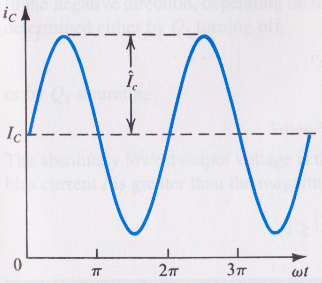
\includegraphics[scale=.35]{valg_af_loesning/klasser/klassea.png}
\caption{Klasse A $i_c$ karakteristik}
\label{fig:klassea}
\end{minipage}
\hspace{0.5cm}
\begin{minipage}[b]{0.5\linewidth}
\centering
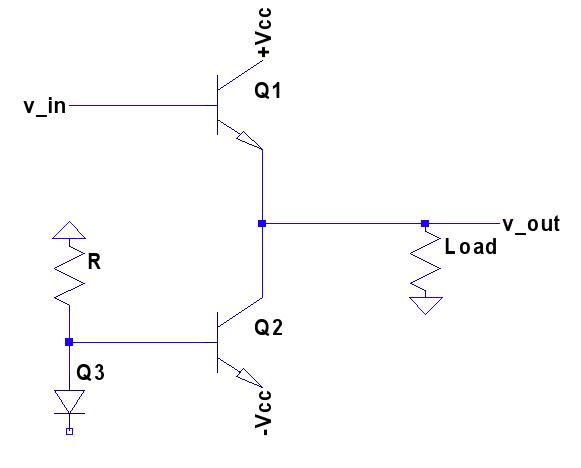
\includegraphics[scale=.35]{valg_af_loesning/klasser/classa.png}
\caption{Et eksempel på et klasse A forstærker kredsløb}
\label{fig:classa}
\end{minipage}
\end{figure}
\fixme{kilde: til sedra smith}


Et klasse A trin har en strømvinkel på udgangstransistoren på 360°. Dette viser sig nyttigt i det at indgangssignalet er repræsenteret på udgangen i sin komplette form, hvilket giver en lav forvrængning.
I et klasse A trin løber altid en konstant strøm gennem Q2, hvis kredsløbet på figur \ref{fig:classa} benyttes. Dette gør at den maksimale teoretiske virkningsgrad kun er 25\%. \fixme{kilde: til sedra smith}

Et klasse A udgangstrin kan opbygges af to NPN transistorer, Q1 og Q2, i en emitterfølgerkobling, som vist på figur \ref{fig:classa}. En konstant strøm løber gennem Q2, da $v_{BE2}$ er konstant. Inputsignalet kommer ind på Q1's base og styrer således strømmen der kan løbe gennem Q1 og loadmodstanden. 



\subsection{Klasse B}

Et klasse B udgangstrin har en strømkarakteristik på udgangen, som vist på figur \ref{fig:klasseb} med en sinustone, som indgangssignal. 

\begin{figure}[ht]
\begin{minipage}[b]{0.5\linewidth}
\centering
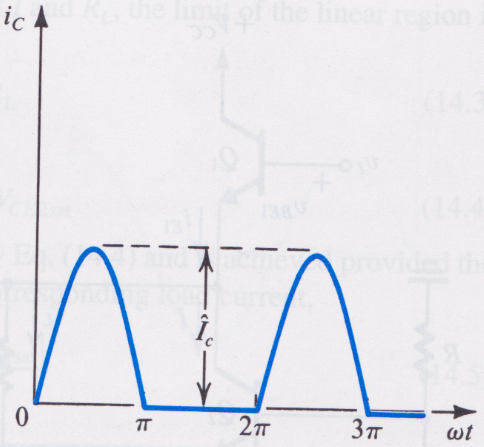
\includegraphics[scale=.35]{valg_af_loesning/klasser/klasseb.png}
\caption{Klasse B $i_c$ karakteristik}
\label{fig:klasseb}
\end{minipage}
\hspace{0.5cm}
\begin{minipage}[b]{0.5\linewidth}
\centering
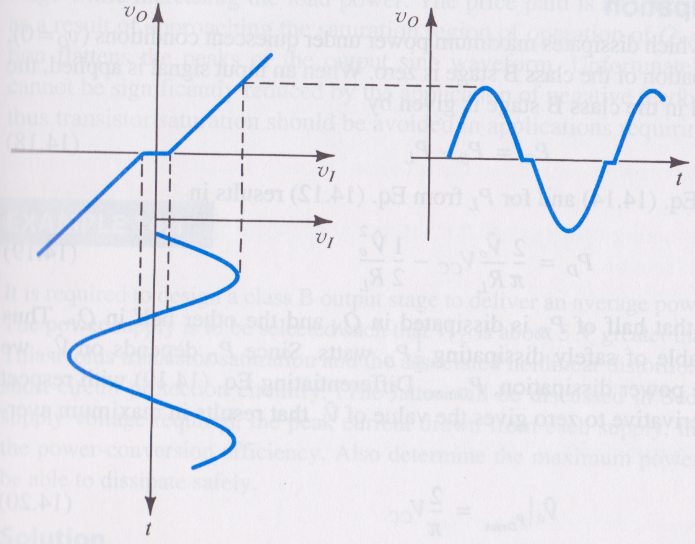
\includegraphics[scale=.25]{valg_af_loesning/klasser/klassebproblem.png}
\caption{Klasse B trin med crossoverdistortion}
\label{fig:classbproblem}
\end{minipage}
\end{figure}
\fixme{kilde: til sedra smith}
Et klasse B trin overfører kun en halv periode af indgangssignalet til udgangen, altså er strømvinklen 180°. For at kunne gengive et udgangssignal similært til indgangssignalet er det derfor nødvendigt at sammensætte to klasse B trin således at det ene tager sig af den positive halvperiode og den anden den negative. Dette giver anledning til et fænomen kaldet crossoverdistortion. Dette fænomen optræder i dette tilfælde i overgangen fra den positive halvperiode til den negative og skyldes diodekarakteristikken i transistorernes base-emitter. Crossoverdistortion for et klasse B trin er illustreret på figur \ref{fig:classbproblem}.
Et klasse B trin har en maksimal nyttevirkning på 78,5 \%.\fixme{kilde: til sedra smith}

I eksemplet er klasse B trinnet opbygget af to transistorer, en NPN (Q1) og en PNP (Q2), som vist på figur \ref{fig:classb}. Når input spændingen overstiger ca. 0,6 V vil Q1 begynde at lede strøm til loadmodstanden mens Q2 er lukket. Kommer input spændingen under -0,6 V vil Q2 lede, men da Q2 er en PNP vil den trække strøm mod -Vcc hvormed der trækkes strøm fra loadmodstanden. Når Q2 leder er Q1 lukket. 

\begin{figure}[h]
\centering
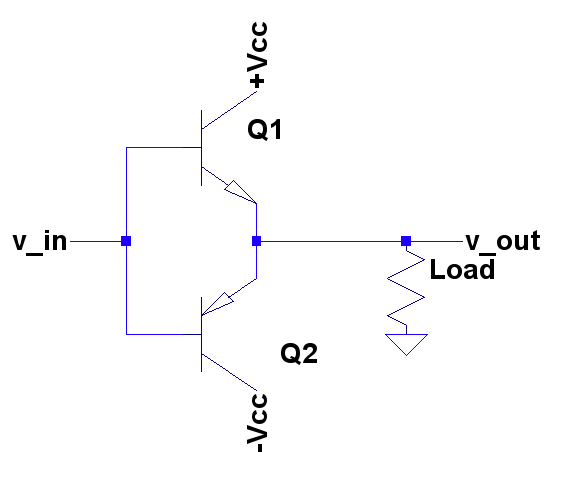
\includegraphics[scale=.35]{valg_af_loesning/klasser/classb.png}
\caption{Klasse B forstærker kredsløb}
\label{fig:classb}
\end{figure}

\subsection{Klasse AB}

Et klasse AB udgangstrin har en strømkarakteristik på udgangen, som vist på figur \ref{fig:klasseab} med en sinustone, som indgangssignal. 

\begin{figure}[ht]
\begin{minipage}[b]{0.5\linewidth}
\centering
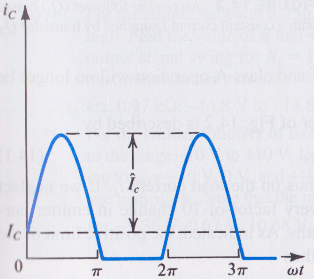
\includegraphics[scale=.35]{valg_af_loesning/klasser/klasseab.png}
\caption{Klasse AB $i_c$ karakteristik}
\label{fig:klasseab}
\end{minipage}
\hspace{0.5cm}
\begin{minipage}[b]{0.5\linewidth}
\centering
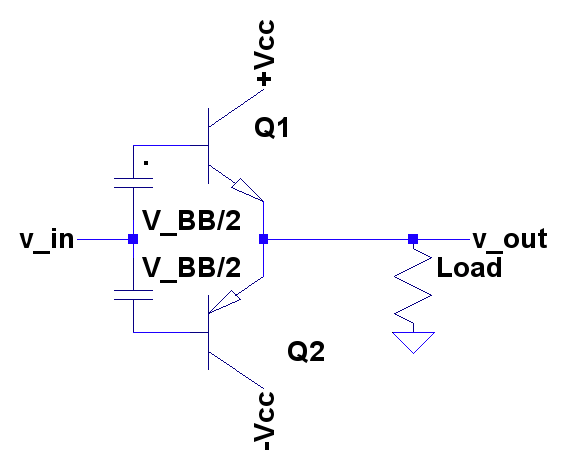
\includegraphics[scale=.35]{valg_af_loesning/klasser/classab.png}
\caption{Klasse AB forstærker kredsløb}
\label{fig:classab}
\end{minipage}
\end{figure}
\fixme{kilde: til sedra smith}


Dette trin har en strømvinkel på mellem 180 ° og 360 °. Dette bevirker at, hvis man bruger samme teknik, som ved et klasse B trin til at få en hel sinusperiode på udgangen, vil de to signaler overlappe i overgangsperioden. Dette medvirker til at crossoverdistortion, som forklaret for klasse B trinnet, elemineres. Dermed bliver forvrængningen for et klasse AB mindre end for et klasse B.
Et klasse AB trin har en nyttevirkning som ligger mellem den for et klasse A og et klasse B. \fixme{kilde: Jan ???}

Der tages i eksemplet på et klasse AB trin på figur \ref{fig:classab} udgangspunkt i klasse B trinnet på figur \ref{fig:classb}, med den forskel at potentialet på Q1 og Q2's base er hævet til saturationspændingen når signalspændningen er 0 V. Det er denne forskel, som eleminerer crossoverdistortion.

Et klasse AB udgangstrin har ikke et klasse A's lave nyttevirkning eller et klasse B's crossoverdistortion og er på baggrund af dette blevet valgt, som det udgangstrin der vil blive arbejdet videre på.
\section{Indgangsvælger}
\begin{frame}{Indgangsvælger - Krav}
\scriptsize{
\begin{table}[h]
\centering
\begin{tabular}{l|r}
\hline\hline
Område & Krav \\
\hline\hline
Antal trin i & 4 \\
indgangsvælgeren & \\[4pt]
Indgangsimpedans & \> 22 k\ohm \\[4pt]
Frekvensgang & \< 0,375 dB ved 20 Hz - 20 kHz, ref. 1 kHz \\
& \< 0,75 dB fra 20 Hz til 63 Hz \\
& \< 0,75 dB fra 12,5 kHz til 20 kHz \\[4pt]
Dæmpning af slukket & \> 50 dB ved 1 kHz \\
indgangssignal & \\
\hline\hline
\end{tabular}
\label{tab:krav_indgangsvaelger}
\end{table}
}
\end{frame}

\begin{frame}{Indgangsvælger - Opbygning}

\begin{figure}[h]
\centering
\includegraphics[width=\textwidth]{../rapport/teknisk/indgangsvaelger/signal-taend-sluk.png}
\label{fig:indgangsvaelger-overordnet}
\end{figure}
\end{frame}

\begin{frame}{Indgangsvælger - Styring}

\begin{figure}[h]
\centering
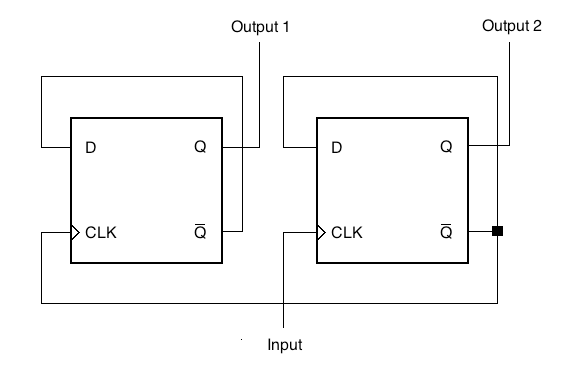
\includegraphics[scale=0.4]{../rapport/teknisk/indgangsvaelger/flipflop.png}
\label{fig:indgangsvaelger-flipflop}
\end{figure}
\end{frame}

\begin{frame}{Indgangsvælger - Simulering}
\begin{figure}[h]
\centering
\includegraphics[width=\textwidth]{../rapport/teknisk/indgangsvaelger/simulering/frekvenskarakteristik.png}
\label{indgangsvaelger_frekvenskarakteristik}
\end{figure}
\end{frame}

\begin{frame}{Indgangsvælger - Måling}
\begin{figure}[h]
\centering
\includegraphics[width=\textwidth]{../rapport/maalerapporter/indgangsvaelger/Indgangsvlger-mic-200mv-frek.png}
\label{fig:indacc:frek200mv}
\end{figure}
\end{frame}

\begin{frame}{Indgangsvælger - Måling}
\begin{figure}[h]
\centering
\includegraphics[width=\textwidth]{../rapport/maalerapporter/indgangsvaelger/Indgangsvlger-mic-2v-thd.png}
\label{fig:accind:thd2v}
\end{figure}
\end{frame}


\begin{frame}{Indgangsvælger - Oversigt}
\scriptsize{
\begin{table}[h]
\centering
\begin{tabular}{l|r|r}
\hline\hline
Område & Krav & Status \\
\hline\hline
Antal trin i & 4 & \checkmark \\
indgangsvælgeren & \\[4pt]
Indgangsimpedans & \> 22 k\ohm & \checkmark \\[4pt]
Frekvensgang & \< 0,375 dB ved 20 Hz - 20 kHz, ref. 1 kHz & \checkmark \\
& \< 0,75 dB fra 20 Hz til 63 Hz & \checkmark\\
& \< 0,75 dB fra 12,5 kHz til 20 kHz & \checkmark\\[4pt]
Dæmpning af slukket & \> 50 dB ved 1 kHz & \checkmark \\
indgangssignal & \\
\hline\hline
\end{tabular}
\label{tab:krav_indgangsvaelger}
\end{table}
}
\end{frame}
\section{Volumenkontrol}
\label{valg_volumenkontrol}
Kravet til styringen af volumenkontrol er sat til at dette skal foregå digitalt. Begrundelsen herfor ligger i projektets undertema, $"$High Fidelity (Hi-Fi) forstærker med digital styring$"$, og begrundes derfor ikke yderligere. Til bestemmelse af den maksimale dæmpning volumenkontrollen skal være i stand til, bruges samme krav som for slukkede signaler, altså 50 dB, som bestemt i afsnit \ref{standarder}. Volumenkontrollen skal derfor kunne dæmpe fra  0 dB til 50 dB. Desuden vælges størrelsen af hvert niveau til 1 dB, da dette er den mindste forskel et menneske kan opfatte i lydniveau \cite{lidt_om_lyd}. Dette sætter ydermere krav til at displayet, som opbygges af 7-segmenter, skal bestå af to 7-segmenter.\\
Volumen skal kunne justeres via trykknapper på HiFi-forstærkerens frontpanel, hvor det også skal være muligt at aflæse det øjeblikkelige volumenniveau.  

\section{Equalizer}
\label{equalizer}
Det menneskellige øre kan opfatte frekvenser fra ca. 20-20k Hz\fixme{kilde: http://www.hoerelse.info/page.dsp?page=414}. Dette sætter en naturligt bredde for frekvensbåndet, forstærkeren skal kunne operere indenfor. Udover at en given elektrisk komponent ikke vil være ens over hele frekvensbåndet, vil det akustiske miljø samt højtalerne også have indflydelse på den endelige oplevelse.  Derfor kan det være nødvendigt at regulere på de forskellige frekvenser, for at opnå den ønskede lyd. En equalizer benyttes til at dæmpe de forskellige frekvensbånd, i forhold til hinanden. En equalizer i en forstærker vil ofte være bredspektret og blive benyttet til at korrigere mere generelle ændringer i lyden. Hvis brugeren ønsker mere specifikke indstillinger, vil en dedikeret equalizer ofte benyttes. Da frekvensbåndet det menneskelige øre kan høre består af præcis 3 dekader, inddeles frekvensbåndene i equalizeren efter disse:
%Udtrykket equalizer stammer fra den originale hensigt med opfindelsen; at få det optagede til at lyde som den originale kilde. Dette gøres bl.a. for at kompensere for unøjagtigheder i optagelsesudstyr. Ved at dæmpe og forstærke individuelle frekvensbånd, er det muligt at få præcis den lyd brugeren kunne tænke sig. 
%En equalizer i en forstærker vil ofte være bredspektret og blive benyttet til at kompensere for det akustiske miljø brugeren befinder sig i, samt unøjagtigheder som følge af de benyttede komponenter. Hvis man har brug for mere specifikke indstillinger vil benyttet en dedikeret equalizer. Derfor har projektgruppen valgt at have 3 frekvensbånd\fixme{kilde: pdf dokument.}.

\begin{itemize}
\item Low: 20 - 200 Hz
\item Mid: 200 - 2000 Hz
\item High: 2000 - 20000 Hz
\end{itemize}

%Frekvensbåndene strækker sig fra 20 Hz til 20 kHz, da dette er det maksimale frekvensbånd det menneskelige øre kan opfatte\fixme{kilde: http://www.hoerelse.info/page.dsp?page=414}. Da dette frekvensbånd består af præcis 3 dekader, har projektgruppen valgt at inddele equalizerens frekvensbånd i disse.
%Hvor mange indstillingmuligheder der er på en equalizer, afhænger af antal af frekvensbånd, som kan indstilles uafhængigt af hinanden. Der opstilles derfor en række frekvensbånd, som et mål for projektet:
%Idéen med en equalizer er at kunne justere på styrken af de forskellige frekvenser i et signal, uafhængigt af hinanden. Dette benyttes til at få præcis den lyd, som brugeren ønsker. Eksempelvis kunne en bruger vælge at skrue op for de lave frekvenser, for at gøre bassen i et signal mere dominerende. I praksis er det dog en kombination af at forstærke nogle frekvensbånd, og dæmpe andre, på tværs af hele det hørbare område, for at skabe nøjagtigt den lyd der ønskes.\fixme{Skriv om} Dette er en hel videnskab i sig selv, men for at gøre mulighederne for dette så store som muligt, er det smart\fixme{andet ord?} at have et bredt udvalg af justerbare bånd. Dette gøres, analogt, ved hjælp af forskellige båndpas filtre.

\subsection{Visualizer}
\label{visualizer}
Visualizeren benyttes til at illustrere styrken af de signalerne i de forskellige frekvensbånd. I teorien kan en analog visualizer have uendeligt stor opløsning. I dette projekt vil det dog ikke give mening, ud fra et læringsmæssigt standpunkt at lave for stor opløsning, da dette bare er gentagelse af de samme basale elementer. Derimod vil en for lav opløsning heller ikke kunne bruges til noget. Derfor er en opløsning på seks dioder pr. frekvensbånd valgt. Dette giver desuden mulighed for at vise signalstyrken med farver: 2 grønne, efterfulgt af 2 gule, efterfulgt af 2 røde dioder.
%En visualizer giver et visuelt udtryk for, hvordan equalizeren er indstillet. Den angiver lydniveauet for hvert frekvensbånd, equalizeren dækker over. Dette giver bl.a. brugeren mulighed for at se hvilke frekvenser, der vil være optimale at justere på, for at få det ønskede output.
Vi startede ud med at beslutte os for, at måden vi skulle dæmpe signalet på, var at trække det til stel, før det blev summeret i summationsforstærkeren. Dette gave os at vi skulle have R3 og R4, for at kunne dæmpe signalet, uden at trække det endelige output til stel. Outputtet fra en gate er 5V, hvilket giver os V2. Der skal desuden løbe en basis strøm I_B, hvilket giver os modstanden R5. C1 er der for kun at få signalet over i indgangsvælger trinet. Vi fandt dog rimeligt hurtigt ud af at et spændingsving omkring 0V ville give prolemer med strøm løbende fra emitteren til collectoren i Q1, når signalet trækkes under 0V. Derfor blev vi enige om at lave et DC offset, hvilket vi gjorde med R1 og R2 samt V1. R1 og R2 er valgt til 100k hver, hvilket giver en spændingsdeling på 1:2 imellem dem, hvilket ved 15V giver et DC offset på 7.5V. R3 og R4 er valgt efter at have en indgangsimpedans over 22, både når indgangen er tændt og slukket. For at regne på dette AC mæssigt, kortsluttes kondensatorerne, hvilket betyder at R1 og R2 begge går til stel. Derfor sidder de i parallel, sammen med Re, som består af R3 og R4 i serie. Ved et slukket signal er der ideelt stel mellem R3 og R4, derfor er R4 ligegyldig her. For at regne R3 opstilles der en parallelkoblingsformel:
\begin{equation}
\frac{1}{\frac{1}{100}+\frac{1}{100}+\frac{1}{R}}=22
R=39.29
\end{equation}
Dette giver altså en R på ca. 40k, når signalet skal slukkes, hvilket altså vil sige R3. Når signalet så er tændt igen, er indgangsimpedansen højere, da R3 og R4 skal adderes. Vi har valgt en R4 på ca 7k, hvilket giver en total indgangsimpedans på:
\begin{equation}
\frac{1}{\frac{1}{100}+\frac{1}{100}+\frac{1}{40.2+7.32}}=24.36
\end{equation}
\section{Udgangseffekt}
\label{valg_udgangseffekt}
Fastsættelsen af udgangseffektens størrelse er bestemt af to faktorer. Den maksimale effekt der er mulig er bestemt af sikkerhedsreglerne i elektroniklaboratoriet på Aalborg Universitet. I disse regler angives den maksimale DC spænding der må arbejdes med til 60 V \cite{elregler-b1101}. 
Til projektets forstærker deles denne spænding til en forsyning som maksimalt kan være $\pm$ 30 V. Under udregningen af den maksimale effekt bruges RMS-værdien af den spænding. Desuden anvendes den, i afsnit \ref{standarder} valgte, belastningsmodstand på 8~\ohm. Dermed bliver den øvre grænse som vist i udregningen i formel (\ref{equ:maks_effekt}).

\begin{equation}
\label{equ:maks_effekt}
P_{\mathrm{max}} = \frac{(V_{\mathrm{RMS}})^2}{R_{\mathrm{load}}}= \frac{(\frac{\hat{V}}{\sqrt{2}})^2}{R_{\mathrm{load}}} = \frac{(\frac{\mathrm{30~V}}{\sqrt{2}})^2}{8~\ohm} = \mathrm{56,25~W}
\end{equation}

Den nedre grænse for udgangseffekten er defineret af standarden IEC581, i hvilken det er bestemt at udgangseffekten som minimum skal være 10 W, hvis der er tale om en monoudgang, før forstærkeren må kaldes en HiFi-forstærker, se afsnit \ref{standarder}. Kravet for udgangseffekten vælges til 20 W for dette projekts HiFi-forstærker.

\section{Kortslutningssikring}
\label{valg_kortslutningssikring}
Der er opstillet krav om en kortslutningssikring for at sikre mod skader ved eventuelle overbelastninger på udgangen af HiFi-forstærkeren. Afsættes der $20~W$ i højtaleren, kan peakstrømmen bestemmes ved beregningen vist i formel (\ref{equ:ipeak}).

\begin{equation}
\label{equ:ipeak}
I_{\mathrm{peak}} = \sqrt{2 \cdot \frac{p_{\mathrm{RMS}}}{R}} = \sqrt{2 \cdot \frac{\mathrm{20~W}}{8~\ohm}}  = \mathrm{2,24~A}
\end{equation}

Denne peakstrøm fremkommer ved peakspændingen fundet i udregningen i formel (\ref{equ:vpeak}).

\begin{equation}
\label{equ:vpeak}
V_{\mathrm{peak}} = I_{\mathrm{peak}} \cdot R_{\mathrm{load}} = \mathrm{2,24~A \cdot 8~\ohm = 17,9~V}
\end{equation}

Ideelt vil en spændingsforsyning på 18 V altså være tilstrækkelig, dog er der rent praktisk behov for en større. Argumentationen herfor findes i afsnit \fixme{ref til udregninger ved effektforstærker}, hvor den ydermere bestemmes.
\section{Udgangssignaltype}
\label{valg_udgangssignaltype}
Valget står for udgangssignaltypen mellem stereo og mono. Da stereo i princippet blot er et lydsignal med to kanaler i modsætning til mono, som er én kanal, vil fremstillingen af en stereoudgang på forstærkeren ikke umiddelbart være mere lærerig end fremstillingen af en monoudgang, den vil blot kræve mere tid. Af den årsag vælges udgangssignaltypen til mono.
\section{Total Harmonic Distortion}
\label{thd}
Total Harmonic Distortion, total harmonisk forvrængning - forkortet THD - er et udtryk for hvor meget forvrængning der er i et signal, fra kilden til output.  Hele kæden er med til at øge THD, da det er et biprodukt af, at komponenter ikke er lineære og derfor vil tilføje forvrængning til signalet. Jo højere THD, jo kraftigere overtoner, kendt på engelsk som harmonics\fixme{evt. i fodnote eller ordforklaring i stedet?}, vil der blive produceret, hvilket vil ændre det originale signal. Overtoner er frekvenser, som har et heltalsforhold\fixme{er det et ord?} til den originale frekvens; eksempelvis vil overtoner til 500Hz være 1000Hz, den dobbelte frekvens, og 1500Hz, tre gange frekvensen.\fixme{Skriv om med ligning} Disse overtoner bliver lagt til det originale signal; dette svarer til at det originale signal, er en slags AC-offset til de mindre kraftige overtoner, som set i figur \fixme{figur}. Det er derfor vigtigt at få så lav forvrængning som muligt, da hvert enkelt led i kæden, bidrager med sin egen. Så længe HiFi-forstærkerens totale forvrængning er under 1\% anses den dog som værende underordnet, da det ikke er muligt at detektere med det menneskelige øre.\fixme{kilde eller lav en ref til standarder}

\begin{figure}[h]
\centering
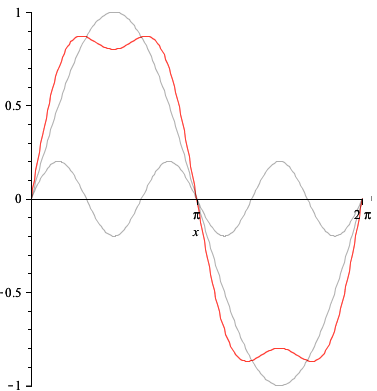
\includegraphics[scale=.4]{indledende_analyse/thd/thdsamlet.png}
\caption{Et eksempel på harmonisk forvrængning. Det originale signal virker som et AC-offset for den mindre kraftige, tredje harmoniske overtone.}
\label{fig:harmonic_distortion}
\end{figure}

%Kravspecifikation
\chapter{Kravspecifikation}
\label{kravspec}
Formålet med dette kapitel er til slut at opstille en kravspecifikation for projektets HiFi-forstærker. Alle kravene i kravspecifikationen skal være målbare, så de kan testes ved projektets afslutning, og begrundede i det omfang dette er muligt. Før det er muligt at opstille en sådan kravspecifikation, er det nødvendigt at dokumentere hvilke overvejelser som danner grundlag for de forskellige dele af kravspecifikationen. Der er i kapitel \ref{kap:indledende_analyse} ført dokumentation for en række af disse overvejelser. De resterende overvejelser er dokumenteret i de næste syv afsnit. I afsnit \ref{krav_krav} er produktet af alle disse overvejelser samlet i den endelige kravspecifikation for projektets HiFi-forstærker. 

\section{Indgangsvælger}
\label{krav_indgangsvaelger}
I forbindelse med indgangsvælgeren er overvejelserne gået på, hvorvidt denne skal lave en trinvis eller flydende overgang mellem indgangssignalerne. Da en flydende overgang i princippet er simultan volumenkontrol af indgangene, adskiller den form for indgangsvælger sig ikke i samme grad fra en egentlig volumenkontrol, som det er tilfældet med en trinvis indgangsvælger. Eftersom der er opstillet krav om en volumenkontrol til forstærkeren sættes kravet om indgangsvælgerens art til trinvis. \\
Som det fremgår i afsnit \ref{standarder} skal HiFi-forstærkeren have to indgange, hvilket danner grundlag for at kravet til antallet af trin i indgangsvælgeren sættes til tre. De tre trin er vist i tabel \ref{tab:indgangsvaelgertrin}.\fixme{Jesper: Har ikke lavet det med isolation, da jeg vil vente og se hvad Jacob skriver om det - ¿ Mener jeg hørte han fandt noget med det til standarder ?}

\begin{table}[h]
\centering
\begin{tabular}{c|c|c}
\hline\hline
Trin & Indgang 1 & Indgang 2 \\
\hline\hline
1 & On & Off \\
2 & Off & On \\
3 & On & On \\
\hline\hline
\end{tabular}
\caption{Indgangsvælgertrin}
\label{tab:indgangsvaelgertrin}
\end{table}

Valget mellem de tre trin skal kunne tages af brugeren på HiFi-forstærkerens frontpanel. Det skal desuden være tydeligt hvilket trin indgangsvælgeren er sat på.

\section{Indgangsimpedans}
\label{krav_indgangsimpedans}
Indgangsimpedansen er at opfatte som en impedans der, ud fra en almindelig spændingsdeling, reducerer indgangssignalet. Man er, med den begrundelse, interesseret i en stor indgangsimpedans. Den mindste tilladte størrelse af indgangsimpedansen for en HiFi-forstærker er i standard IEC61938-1 bestemt til 22 k\ohm~ for liniesignalsindgange, se afsnit \ref{standarder}. Da størrelsen af udgangsimpedansen samtidig er bestemt til maksimalt 2,2 k\ohm~ for en liniesignalsudgang, kan betydningen af indgangsimpedansens størrelse regnes som vist i udregningen i formel (\ref{equ:indgangsimpedans22}). 

\begin{equation}
\label{equ:indgangsimpedans22}
\frac{22~k\ohm}{22~k\ohm + 2,2~k\ohm} = 0,91
\end{equation}

Det ses af udregningen i formel (\ref{equ:indgangsimpedans22}), at en indgangsimpedans af størrelsen 22 k\ohm~ vil medføre et indgangssignal på 91 \% af det oprindelige signal. Med en større indgangsimpedans vil en større del af det oprindelige signal blive indgangssignalet. 

\begin{equation}
\label{equ:indgangsimpedans475}
\frac{47,5~k\ohm}{47,5~k\ohm + 2,2~k\ohm} = 0,96
\end{equation}

Udregningen i formel (\ref{equ:indgangsimpedans475}) viser at med en indgangsimpedans af størrelsen 47,5 k\ohm~ bliver indgangssignalet 96 \% af det oprindelige signal.

\section{Volumenkontrol}
\label{krav_volumenkontrol}
Kravet til styringen af volumenkontrol er sat til at dette skal foregå digitalt. Begrundelsen herfor ligger i det samtidige krav om volumenkontrol via fjernbetjening, læs mere herom i afsnit \ref{krav_fjernbetjening}. Volumen skal desuden kunne justeres via HiFi-forstærkerens frontpanel, hvor det også skal være muligt at aflæse det øjeblikkelige volumenniveau.  

\section{Udgangssignaltype}
\label{krav_udgangssignaltype}
Valget står for udgangssignaltypen mellem stereo og mono. Da stereo i princippet blot er et lydsignal med to kanaler i modsætning til mono, som er én kanal, vil fremstillingen af en stereoudgang på forstærkeren ikke umiddelbart være mere lærerig end fremstillingen af en monoudgang, den vil blot kræve mere tid.

\section{Udgangseffekt}
\label{krav_udgangseffekt}
Fastsættelsen af udgangseffektens størrelse er bestemt af to faktorer. Den maksimale effekt der er mulig er bestemt af sikkerhedsreglerne i elektronikværkstedet på Aalborg Universitet. I disse regler angives den maksimale DC spænding der må arbejdes med til 60 V \cite{elregler-b1101}. 
Til projektets forstærker deles denne spænding til en $\pm$30 V forsyning. Under udregningen af den maksimale effekt bruges RMS-værdien (Root Mean Square) af den spænding. Dermed bliver den øvre grænse som vist i udregningen i formel (\ref{equ:maks_effekt}).

\begin{equation}
\label{equ:maks_effekt}
P_{maks} = \frac{(V_{RMS})^2}{R}= \frac{(\frac{\hat{V}}{\sqrt{2}})^2}{R} = \frac{(\frac{30~V}{\sqrt{2}})^2}{8\ohm} = 56,25~W
\end{equation}

Den nedre grænse for udgangseffekten er defineret af standarden IEC581, i hvilken det er bestemt at udgangseffekten som minimum skal være 10 W hvis der er tale om en monoudgang før forstærkeren må kaldes en HiFi-forstærker, se afsnit \ref{standarder}.

\section{Kortslutningssikring}
\label{krav_kortslutningssikring}
Der er opstillet krav om en kortslutningssikring for at sikre mod skader ved eventuelle overbelastninger på udgangen af HiFi-forstærkeren.

\section{Fjernbetjening}
\label{krav_fjernbetjening}
Fjernbetjeninger har været en del af radio- og tv-udstyr i mere end 70 år og det har i en årrække været mere eller mindre uhørt at producere produkter af den slags uden en fjernbetjening.
Antallet af kontrolmuligheder via fjernbetjeningen er som oftest større eller som minimum det samme som på selve apparatet.\\
Ud fra disse observationer skal dette projekts HiFi-forstærker have en fjernbetjening, med mulighed for at styre de samme ting som på selve forstærkerens frontpanel, hvilket vil sige fjernbetjeningen skal give mulighed for at vælge indgang og volumeniveau. Desuden opstilles et krav om at fjernbetjeningen skal have en rækkevidde på minimum 1 meter.

\section{Endelig kravspecifikation}
\label{krav_krav}
Tabel \ref{tab:kravspec} viser hvilke krav der er stillet til dette projekts HiFi-forstærker. Tabellen viser desuden videre til hvilke overvejelser eller standarder, der danner grundlag for hvert enkelt krav.

\begin{table}[h]
\centering
\begin{tabular}{l|r|l}
\hline\hline
Område & Krav & Baggrund for krav \\
\hline\hline
\textbf{Teknisk:} & & \\
Forstærkerklasse & AB & Se afsnit \ref{klasser} \\
Total Harmonic Distortion & \color{red}{<1 \%} & Ref til THD afsnit \\
Indgange & Linie og mikrofon & Se afsnit \ref{standarder} \\
Indgangsvælger & 3 trin & Se afsnit \ref{krav_indgangsvaelger} \\
Indgangsimpedans & > 22 k\ohm ($\pm$ 1 \%) & IEC61938-1 samt afsnit \ref{krav_indgangsimpedans} \\
Equalizer-niveauer & \color{red}{?} & Ref til equalizer afsnit \\
Volumenkontrol & Digital & Se afsnit \ref{krav_volumenkontrol} \\
Udgangseffekt & 20 W ($\pm$ 2 W) i 8~$\Omega$ & IEC581, DIN45500 samt afsnit \ref{krav_udgangseffekt} \\
Udgangssignaltype & Mono & Se afsnit \ref{krav_udgangssignaltype} \\
Udgangsimpedans & < 2,2 k\ohm & IEC61938-1 samt afsnit \ref{standarder} \\
Kortslutningssikring & Ja & Se afsnit \ref{krav_kortslutningssikring} \\
\hline
\textbf{Frontpanel:} & & \\
Indgangsvælger & Ja & Se afsnit \ref{krav_indgangsvaelger} \\
Volumenkontrol & Ja & Se afsnit \ref{krav_volumenkontrol} \\
Volumedisplay & Ja & Se afsnit \ref{krav_volumenkontrol} \\
Visualizer & Ja & Ref til visualizer underafsnit \\
\hline
\textbf{Fjernbetjening:} & & \\
Volumenkontrol & Ja &  Se afsnit \ref{krav_fjernbetjening}\\
Indgangsvælger & Ja &  Se afsnit \ref{krav_fjernbetjening}\\
Rækkevidde & 1 m & Se afsnit \ref{krav_fjernbetjening}\\
\hline\hline
\end{tabular}
\caption{Samlet kravspecifikation}
\label{tab:kravspec}
\end{table}

Med denne kravspecifikation er der nu grundlag for at udvikle og fremstille en HiFi-forstærker.

%Tekniske afsnit

%Forforstærker
\section{Forforstærker}

\begin{frame}{Forforstærker}
\begin{itemize}
\item Forstærke signal fra mikrofon
\item Mikrofon: MCE-4000
\item Mikrofons output spænding: 0,8 - 200 mV
\item Output som skal opnås: 200 mV - 2 V
\item Lineær forstærkning ikke muligt
\item Valgte peakspændinger beregnet ud fra forventeligt lydtryk
\end{itemize}
\end{frame}

\begin{frame}{Forforstærker - krav}
\begin{itemize}
\item Indgangsimpedans: 22 k\ohm
\item Frekvensgang: 
\begin{itemize}
\item  under 0,375 dB ved 20 Hz - 20 kHz, ref. 1 kHz 
\item  under 0,75 dB fra 20 Hz til 63 Hz 
\item  under 0,75 dB fra 12,5 kHz til 20 kHz
\end{itemize}
\item Forvrængning: < 0,5 \%
\item Forstærkning: 69,7 gange ved 22k\ohm indgangsimpedans og ved 1 kHz
\end{itemize}
\end{frame}

\begin{frame}{Forforstærker - opbygning}
\begin{itemize}
\item To common-emitter forstærkere med uafkoblet emittermodstand
\item Der vælges to trin for at opnå en stor mængde tilbagekobling
\item 
\item Output som skal opnås: 200 mV - 2 V
\item Lineær forstærkning ikke muligt
\item Valgte peakspændinger beregnet ud fra forventeligt lydtryk
\end{itemize}
\end{frame}
\section{Design}
I dette projekt er der valgt så vidt muligt at designe alle løsninger med diskret elektronik. Derfor er det valgt at forforstærkeren bygges af commonemittertrin med uafkoblet emittermodstand. Et commonemittertrins typiske opbygning er vist på figur \ref{fig:cekobling}.

\begin{figure}[h]
\centering
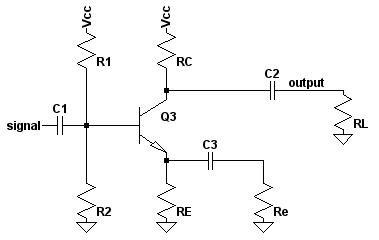
\includegraphics[scale=.6]{teknisk/forforstaerker/ceopkobling.png}
\caption{Generel form på commonemitterkobling med uafkoblet emittermodstand}
\label{fig:cekobling}
\end{figure}


Argumentet for dette valg er at det er det eneste trin, blandt commonemitter, -base og -collector, hvis spændingsforstærkning er betydeligt over én og ikke, under korrekte omstændigheder, afhænger af transistorparametre. Da transistorparametre blandt andet er afhængige af den anvendte transistors temperatur er det en betragtelig styrke ikke at skulle tage højde for dem. Spændingsforstærkningen i commonemittertrinnet er dog kun uafhængig af transistorparametre så længe følgende er gældende: $r_o >>R_C \| R_L$, $gm \cdot R_E||R_e$ og $i_e \approx i_c$.
Dette skyldes at forstærkningen er givet ved ligning (\ref{eq:gmbevis}) \cite{ael-mm6}.

\begin{equation}
A_v =  \frac{-gm \cdot R'_L}{1+gm \cdot R'_e} \approx  -\frac{R'_L}{R'_e} \Biggr\vert _{\frac{1}{gm}<<R'_e}
\label{eq:gmbevis}
\end{equation}

Hvor $R'_e = R_e || R_E$ og $R'_L = R_L||R_C$. Det vil sige at jo tættere $R_e$ kommer på $\frac{1}{gm}$ jo mere indflydelse vil denne have på forstærkningen. Disse antagelser vil derfor være gældende gennem hele designet af forforstærkeren. 

Det første trin skal have en forstærkning på 10 gange og det andet på 6,97 for at opnå den ønskede forstærkning, som vist på figur \ref{blok_forforstaerker}. Grunden til rækkefølgen af trinnene er for ikke at have størst signaludsving og den største forstærkning i samme trin. Dette skyldes at der i en forstærker altid vil være forvrængning og støj. Hvis den største forstærkning kommer sidst, vil denne forvrængning blive forstærket yderligere, hvilket ikke er ønskværdigt. Hvis den største forstærkning derimod kommer først, vil der blive mindst muligt forvrængning med i det endelige signal.\fixme{Hvordan viser vi at det er smart? Frederik: Er det godt nok? Skal der skrives mere? Skal der beregninger med, der beviser det? (synes jeg ikke)}

\begin{figure}[h]
\centering
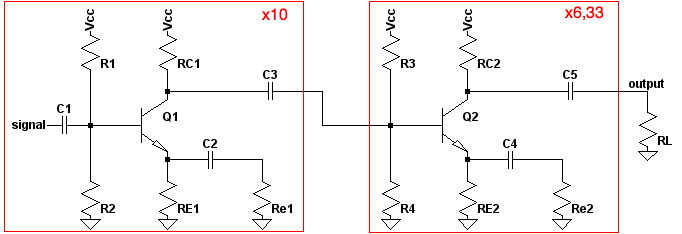
\includegraphics[scale=.6]{teknisk/forforstaerker/blok_forforstaerker.png}
\caption{Blokdiagram over forforstærkerens byggeblokke samt lydsignalets vej}
\label{blok_forforstaerker}
\end{figure}

For at opnå så lav forvrængning som muligt designes hvert trin således at forstærkningen, uden den AC-koblede emittermodstand $R_e$, er så stor som muligt for at gøre tilbagekobling muligt. For derefter at få den ønskede forstærkning tilføjes tilbagekoblingsmodstanden $R_e$.

\subsection*{Design af første trin}
Begge trin designes efter maksimal forstærkning uden $R_e$. Denne forstærkning er givet ved ligning (\ref{eq:dcgain}).

\begin{equation}
|A_{vs}|=\frac{1}{\left(\frac{V_T \cdot R_C}{V_{R_C}}+\frac{R'_S}{\beta}\right) \left(\frac{1}{R_C}+\frac{1}{R_L}\right)}
\label{eq:dcgain}
\end{equation}
Hvor $R'_S = R_S||R_1||R_2$ og $V_T = 26 \cdot 10^{-3}$.

For at designe et kredsløb med maksimal forstærkning justeres størrelsen af $R_C$ uden at variere spændingen over den, $V_{R_C}$. Den maksimale $R_C$ findes ved ligning (\ref{eq:rcmaks}).

\begin{equation}
R_{\mathrm{C,maks}} = \sqrt{\frac{R'_S \cdot R_L \cdot V_{R_C}}{\beta \cdot V_T}}
\label{eq:rcmaks}
\end{equation}

I ligning (\ref{eq:rcmaks}) er $R'_S$ defineret som $R_1||R_2||R_S$. $R_S$ er fastlagt til 2,2 k\ohm, hvilket er mikrofonens udgangsimpedans \cite{mic-datablad}. Parallelforbindelsen mellem $R_1$ og $R_2$ kan ikke beregnes men skal vælges. Indgangsimpedansen i kredsløbet, som netop er $R_1||R_2$, skal som hovedregel være meget større end udgangsimpedansen i den kreds den belaster. En tommelfingerregel siger at 10 gange større er tilstrækkeligt til at være $"$meget større$"$ hvormed parallelkoblingen skal være over eller lig med 22 k\ohm. 
Belastningen, $R_L$, for det første trin bliver indgangsimpedansen i det andet. Indgangsimpedansen i det andet trin bliver $R_3||R_4$ og kan heller ikke beregnes. Da $R_C$ i det første trin ikke kendes endnu vælges indgangsimpedansen i det andet til at være den samme som i det første, altså 22 k\ohm. 
$V_{R_C}$ er defineret som værende $V_{CC} - V_{\mathrm{CE,sat}} - V_{R_E} - V_{\mathrm{o,peak}}$, hvor $V_{CC}$ vælges til 15 V så der sikres at der er plads til det ønskede spændingsudsving, $V_{R_E}$ vælges til 3 V og $V_{\mathrm{CE,sat}}$ aflæses i databladet for BC547b \cite{bc547b-datablad} til 0,2 V ved en collectorstrøm på 1 mA. Der antages at collectorstrømmen cirka bliver 1 mA. Ligeledes aflæses $\beta$ til 250 ved 1 mA i databladet. $V_{\mathrm{o,peak}}$ er peakspændingen på udgangen. Dermed bliver peakspændingen en faktor 10 højere end mikrofonens output peakspænding. $V_{\mathrm{o,peak}}$ bliver derfor 316 mV. $R_{C1}$ beregnes hermed i ligning (\ref{eq:rcforsteberegning}).

\begin{equation}
R_{\mathrm{C1}} = \sqrt{\frac{22~k\ohm || 2,2~k\ohm \cdot (15~V - 0,2~V - 3~V - 0,287~V)}{250 \cdot 26 \cdot 10^{-3}}}=8,83~k\ohm
\label{eq:rcforsteberegning}
\end{equation}

$R_{E1}$ bestemmes i ligning (\ref{eq:beregningre1}) under antagelse at $i_e = i_c$.  $i_c$ beregnes i ligning(\ref{eq:ff:ic}).

\begin{equation}
\label{eq:ff:ic}
i_C=\frac{V_{R_C}}{R_C}=\frac{11,5~V}{9,25~k\ohm}=106,4~mA
\end{equation}
\begin{equation}
R_{E1}=\frac{V_{R_{E1}}}{\frac{V_{R_{C1}}}{R_{C1}}}  \Rightarrow R_{E1}=\frac{3~V}{106,4~mA}=2,30~k\ohm
\label{eq:beregningre1}
\end{equation}


Dernæst beregnes $R_{e1}$ ud fra hvad den ønskede forstærkning skal være. Ligning (\ref{eq:gmbevis}) benyttes til at beregne $R_{e1}$ i ligning (\ref{eq:rlilleeberegning}).

\begin{equation}
\label{eq:rlilleeberegning}
A_v = -\frac{R'_L}{R'_e} \Rightarrow  R_{e1} =-\frac{R_L \cdot R_{C1} \cdot R_{E1}}{A_v \cdot R_{E1} \cdot R_{C1} + A_v \cdot R_{E1} \cdot R_L + R_{C1} \cdot R_L} \Rightarrow R_{e1} = 867,6~\ohm
\end{equation}

Biasnetværket, bestående af $R_1$ og $R_2$ beregnes ud fra den spænding, som er påkrævet på basen for at transistoren fungerer som ønsket. Spændingen over base-emitter, $V_{\mathrm{BE}}$ er i databladet aflæst til 0,6 V. Da potentialet på emitteren er 3 V skal potentialet på basen være 3,6 V. $R_1$ og $R_2$ kan beregnes ud fra at $V_{R_2}$ skal være 3,6 V og parallelkoblingen $R_1||R_2$. Beregningen udføres i ligning (\ref{eq:r1r21}) og (\ref{eq:r1r22}).

\begin{equation}
V_{R_2} = V_{CC} \cdot \frac{R_2}{R_1+R_2} 
\label{eq:r1r21}
\end{equation}
\begin{equation}
R_1||R_2 = \frac{R_1 \cdot R_2}{R_1 + R_2}
\label{eq:r1r22}
\end{equation}
De kendte værdier indsættes og de to ligninger med to ubekendte løses. Resultatet er vist i ligning (\ref{eq:r1r2result}).
\begin{equation}
R_1 = 91,7~k\ohm ~ \wedge ~ R_2=28,9~k\ohm
\label{eq:r1r2result}
\end{equation}

For at opnå den ønskede frekvensgang skal $C1$, $C2$ og $C3$ dimensioneres således at den knækfrekvens de hver især frembringer. Da knækfrekvensen er det punkt hvor kurven er faldet 3 dB og frekvensgangen skal, jævnfør kravspecifikationen, være 20 Hz til 20 kHz, er det nødvendigt at knækfrekvens  ligger før 20 Hz. Det vurderes at knækfrekvensen beregnes til at ligge i 2 Hz for at knækfrekvensen ikke giver anledning til en dæmpning af signalet på mere end de tilladte 3 dB.

Kondensatorerne beregnes med formel (\ref{eq:kondensatorknaek}).

\begin{equation}
C=\frac{1}{\omega \cdot R}=\frac{1}{2\cdot \pi \cdot f \cdot R}
\label{eq:kondensatorknaek}
\end{equation}

I ligning \ref{eq:kondensatorknaek} er $C$ kondensatorens capacitet og $R$ er den impedans kondensatoren ser ind i. 
$C1$ ser ind i forspændingskoblingen i det første forstærkertrin, altså 22 k\Ohm. $C2$ ser ind i den AC-koblede emittermodstand, $Re1$. $C3$ ser ind i forspændingsnetværket i det andet forstærkertrin, altså 22 k\Ohm. Dermed bliver kondensatorernes værdier som følger.

\begin{equation}
C1=3,58~\my F~\wedge ~C2=91,9~\my F~\wedge ~C3=3,58~\my F
\end{equation}



\subsection*{Design af andet trin}
Beregning af andet trin følger samme designprocedure som første trin. Kredsløbet til andet trin er vist på figur \ref{fig:andettrinkreds}.

\begin{figure}[h]
\centering
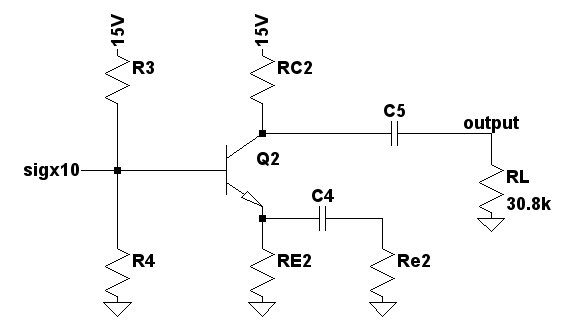
\includegraphics[scale=.6]{teknisk/forforstaerker/andettrinkreds.png}
\caption{Det andet trins kredsløb}
\label{fig:andettrinkreds}
\end{figure}

Det andet trin skal forstærke et signal med en maksimal peakspænding på 287 mV op til 2 V, altså 6,97 gange. Belastningsmodstanden for dette forstærkertrin er bestemt af indgangsvælgeren, som er det næste trin efter forforstærkeren. Indgangsvælgerens indgangsimpedans er 30,8 k\ohm \fixme{reference til indgangsvælgeren hvor det står}. $R_S$ er i dette trin givet ved udgangsmodstanden for det første forstærkertrin, som er lig med $R_{C1}$ hvilket gør at $R'_S = R_{C1} || R_3 || R_4$. Den maksimale $R_{C2}$ beregnes i ligning \ref{eq:rc2maks}.

\begin{equation}
R_{\mathrm{C2}} = \sqrt{\frac{R'_S \cdot R_L \cdot V_{R_C2}}{\beta \cdot V_T}} = 17,1~k\ohm
\label{eq:rc2maks}
\end{equation}

Beregningerne af $R_{E2}$ og $R_{e2}$ samt kondensatorerne er meget ens med dem for det første forstærkertrin. Derfor er det valgt ikke at vise beregningerne i rapporten. $R_3$ og $R_2$ antager samme værdier som henholdsvis $R_1$ og $R_2$, da begge trin skal have samme indgangsimpedans. De beregnede værdier er vist i ligning (\ref{eq:valuestrin2}).

\begin{equation}
R_{E2}=5233,7~\ohm ~ \wedge ~R_{e2}=2599,4~\ohm ~ \wedge ~ C4=30,6~\my F ~ \wedge ~ C5=2,6~\my F
\label{eq:valuestrin2}
\end{equation}

Det endelige kredsløb er vist på figur \ref{fig:forforstaerkersimuleringkredslob} i simuleringsafsnittet.

\subsection*{Simulering}

For at verificere at kredsløbet fungerer som ønsket simuleres det i LTspice. De karakteristika som skal verificeres er spændingsforstærkningen, amplitudekarakteristikken samt harmonisk forvrængning. Kredsløbet der simuleres er vist på figur \ref{fig:forforstaerkersimuleringkredslob}. 

\begin{figure}[h]
\centering
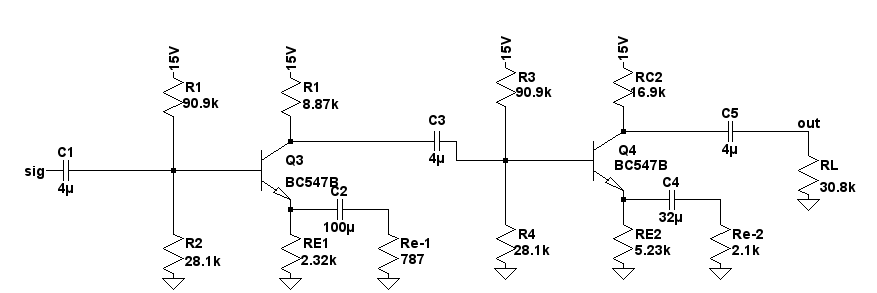
\includegraphics[scale=.6]{teknisk/forforstaerker/forforstaerkerendeligkreds.png}
\caption{}
\label{}
\end{figure}

Spændingsforstærkningen af hele trinnet skal være 69,7 gange svarende til 36,9 dB. Forstærkningen vises på figur \ref{fig:amplitude-forforstaerker} ved hjælp af en amplitudekarakteristik, således at spændet fra 20 Hz til 20 kHz tydeligt kan ses. 


\begin{figure}[h]
\centering
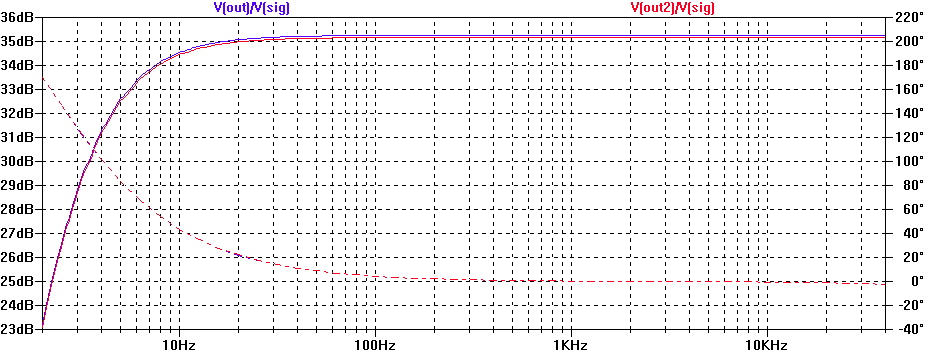
\includegraphics[scale=.6]{teknisk/forforstaerker/amplitudeforforstaerker.png}
\caption{Forforstærkerens amplitude karakteristik}
\label{fig:amplitude-forforstaerker}
\end{figure}

Simuleringen viser at forstærkningen ved 1 kHz, som er referencen jævnfør kravspecifikationen, er 36 dB hvor den skulle have være 36,9 dB. Dermed må der konkluderes at beregningen af forforstærkertrinnene indeholder usikkerheder. Usikkerhederne vurderes til at bestå i de antagelser som defineres før beregningerne: $r_o >>R_C \| R_L$, $gm \cdot R_E||R_e$ og $i_e \approx i_c$. For at korrigere forstærkningen i trinnene kan der, ifølge ligning \ref{eq:gmbevis}, justeres på den AC-koblede emittermodstand, $R_{e1}$ og $R_{e2}$. I ligning \ref{eq:nyerevalues} er de nye værdier for disse modstande anvist. Modstandsværdierne er fundet ved først at justere $R_{e1}$ til det første trin giver den korrekte forstærkning for derefter at gøre det samme med det andet trin.

\begin{equation}
R_{e1}=790~\ohm~\wedge ~R_{e2}=2,1~k\ohm
\label{eq:nyerevalues}
\end{equation}

Med de nye modstandsværdier bliver amplituden som vist på figur \ref{fig:rigtigamplitudeforforstaerker}.

\begin{figure}[h]
\centering
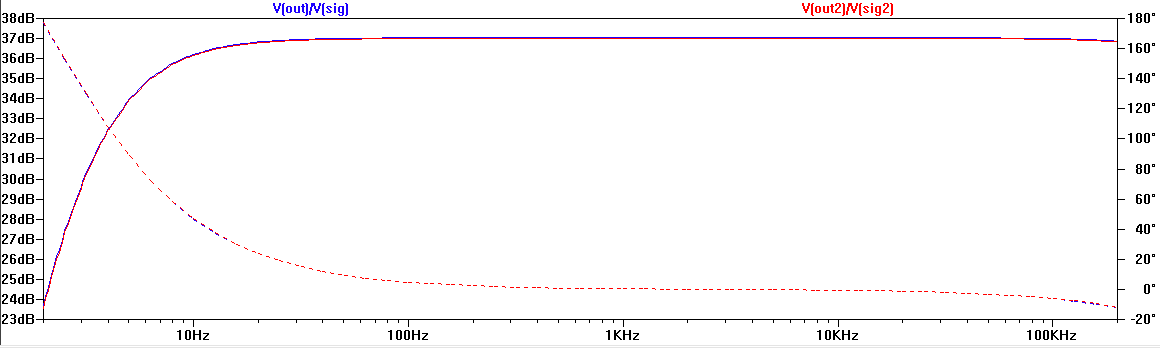
\includegraphics[scale=.6]{teknisk/forforstaerker/rigtigamplitude.png}
\caption{Forforstærkerens amplitudekarakteristik efter korrektion af forstærkning}
\label{fig:rigtigamplitudeforforstaerker}
\end{figure}

På figur \ref{fig:rigtigamplitudeforforstaerker} ses det at forstærkningen nu er korrigeret. Derudover fremgår det at dæmpningen fra 20 kHz til 20 Hz er 0,2 dB. Dermed overholdes kravet om at dæmpningen i dette område, som skal være under 0,375 dB. 

Den harmoniske forvrængning skal ifølge kravspecifikationen være under 0,5 \%. Ifølge LTspice er den harmoniske forvrængning ved 1 kHz og maksimal peakspænding på indgangen 0,18 \%. Forvrængningsmålingen er udført ved maksimal peakspænding da forvrængningen i trinnet vil være mest kritisk i den situation. 







\subsection{Implementering}
Det blev besluttet at benytte potentiometere som $R_e$ modstand ved begge forstærkere, for at kunne indstille forstærkningen. Dette skyldes at meget små afvigelser i modstandsværdien vil betyde en større ændring i forstærkningen. For at kunne opveje dette gøres forstærkningen justerbar, så den kan justeres til den rigtige værdi efter behov. En bivirkning af at justere på $R_e$ vil være mængden af THD, i og med at mængden af tilbagekobling justeres sammen med denne modstand.
\section{Accepttest}
\label{forforstaerker_accepttest}

Kravene specifikt til forforstærkeren er opstillet i tabel \ref{tab:krav_forforstaerker} og med henblik på at teste dem, er der udført målinger som beskrevet i Appendiks D??. Indgangsimpedansen er, som vist i tabel \ref{tab:resultatimpedans_forforstaerker}, med målingerne beregnet til 22,1 k\ohm~. Kravet lyder på 22 k\ohm, hvilket dermed ikke umiddelbart er opnået. Dog kan tolerancen på referencemodstanden alene, på 1\%, som det ses i udregningen i formel (\ref{equ:forforstaerker_ztolerance}), være skyld i dette.

\begin{equation}
\label{equ:forforstaerker_ztolerance}
\vert Z \vert = \frac{\mathrm{14,6~mV}}{\mathrm{6,6~mV}} \cdot \mathrm{10~k\ohm} \pm 1~\% =  \mathrm{22,1~k\ohm} \pm 221~\ohm
\end{equation}

Dette krav betragtes derfor som opfyldt, hvilket kravet om forvrængning også gør. Som det ses på figur \ref{fig:accepttest-thdresultat-forforstaerker} topper denne under 0,25 \% og kravet lyder på maksimalt 0,5 \%. 

\begin{figure}[h]
\centering
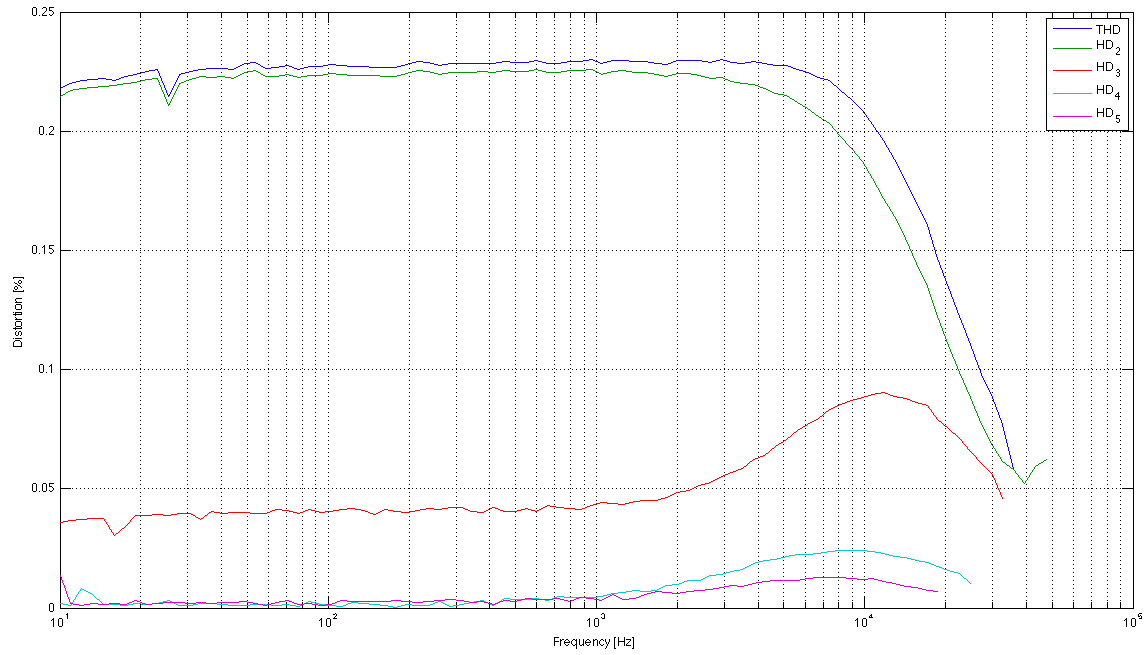
\includegraphics[width=\textwidth]{maalerapporter/forforstaerker/thd-forforstaerker.png}
\caption{Forvrængningsresultat}
\label{fig:accepttest-thdresultat-forforstaerker}
\end{figure}

\begin{figure}[h]
\centering
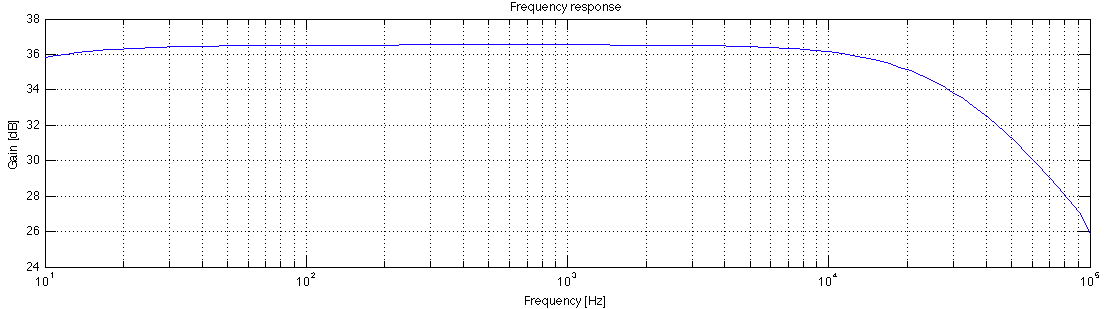
\includegraphics[width=\textwidth]{maalerapporter/forforstaerker/frekvensrespons-forforstaerker.png}
\caption{Frekvensgangs- og forstærkningsresultater}
\label{fig:accepttest-fresultat-forforstaerker}
\end{figure}

Forstærkningen ved 1 kHz er, fra resultaterne afbilledet på figur \ref{fig:accepttest-fresultat-forforstaerker}, 36,54 dB, hvilket i udregningen vist i formel (\ref{equ:accepttest-forforstaerker-db-gange}) omregnes.

\begin{equation}
\label{equ:accepttest-forforstaerker-db-gange}
10^{\frac{\mathrm{36,54~dB}}{20}} = 67,1~gg
\end{equation}

Dette opfylder ikke kravet på 69,7 gange, men resultaterne vurderes alligevel til at være gode. Forskellen tilskrives justeringen af potentiometer under implementeringen. Frekvensgangskravene er, som det kan ses på figur \ref{fig:accepttest-fresultat-forforstaerker}, figur \ref{fig:accepttest-fres-20-63} og figur \ref{fig:accepttest-fres-125-20}, opfyldt pånær kravet ved 12,5 kHz til 20 kHz, hvor den falder 0,8 dB. Dog skulle denne blot være under 0,75 dB for at leve op til kravet, hvormed tolerancer på måleudstyret vurderes at spille ind. Derfor betragtes alle kravene som værende opfyldt.

\begin{figure}[h]
\centering
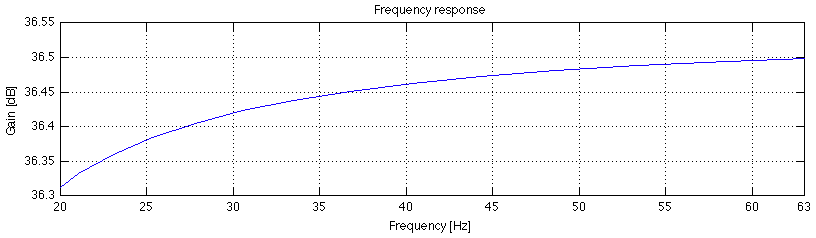
\includegraphics[width=\textwidth]{maalerapporter/forforstaerker/fr20-63.png}
\caption{Frekvensgangsresultater fra 20 Hz til 63 Hz}
\label{fig:accepttest-fres-20-63}
\end{figure}

\begin{figure}[h]
\centering
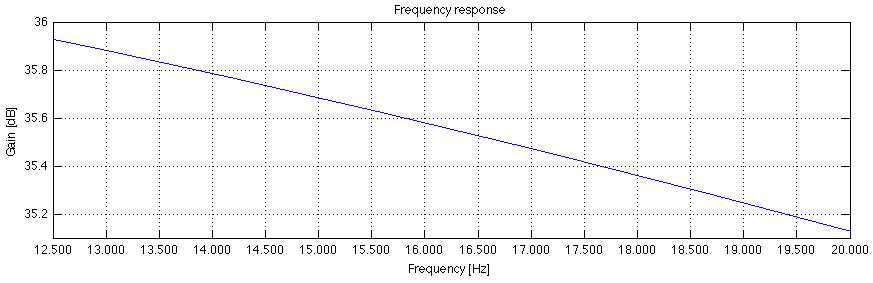
\includegraphics[width=\textwidth]{maalerapporter/forforstaerker/fr12-20k.png}
\caption{Frekvensgangsresultater fra 12,5 kHz til 20 kHz}
\label{fig:accepttest-fres-125-20}
\end{figure}

%Indgangsvælger
\section{Indgangsvælger}
\begin{frame}{Indgangsvælger - Krav}
\scriptsize{
\begin{table}[h]
\centering
\begin{tabular}{l|r}
\hline\hline
Område & Krav \\
\hline\hline
Antal trin i & 4 \\
indgangsvælgeren & \\[4pt]
Indgangsimpedans & \> 22 k\ohm \\[4pt]
Frekvensgang & \< 0,375 dB ved 20 Hz - 20 kHz, ref. 1 kHz \\
& \< 0,75 dB fra 20 Hz til 63 Hz \\
& \< 0,75 dB fra 12,5 kHz til 20 kHz \\[4pt]
Dæmpning af slukket & \> 50 dB ved 1 kHz \\
indgangssignal & \\
\hline\hline
\end{tabular}
\label{tab:krav_indgangsvaelger}
\end{table}
}
\end{frame}

\begin{frame}{Indgangsvælger - Opbygning}

\begin{figure}[h]
\centering
\includegraphics[width=\textwidth]{../rapport/teknisk/indgangsvaelger/signal-taend-sluk.png}
\label{fig:indgangsvaelger-overordnet}
\end{figure}
\end{frame}

\begin{frame}{Indgangsvælger - Styring}

\begin{figure}[h]
\centering
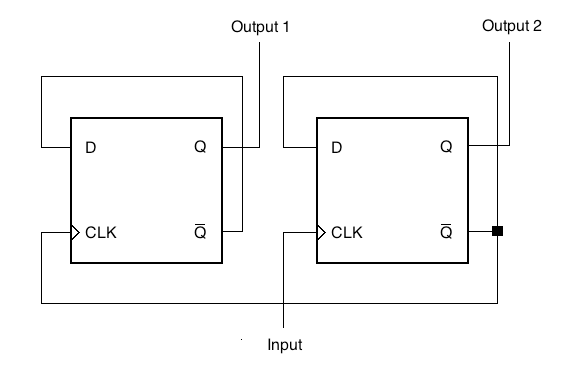
\includegraphics[scale=0.4]{../rapport/teknisk/indgangsvaelger/flipflop.png}
\label{fig:indgangsvaelger-flipflop}
\end{figure}
\end{frame}

\begin{frame}{Indgangsvælger - Simulering}
\begin{figure}[h]
\centering
\includegraphics[width=\textwidth]{../rapport/teknisk/indgangsvaelger/simulering/frekvenskarakteristik.png}
\label{indgangsvaelger_frekvenskarakteristik}
\end{figure}
\end{frame}

\begin{frame}{Indgangsvælger - Måling}
\begin{figure}[h]
\centering
\includegraphics[width=\textwidth]{../rapport/maalerapporter/indgangsvaelger/Indgangsvlger-mic-200mv-frek.png}
\label{fig:indacc:frek200mv}
\end{figure}
\end{frame}

\begin{frame}{Indgangsvælger - Måling}
\begin{figure}[h]
\centering
\includegraphics[width=\textwidth]{../rapport/maalerapporter/indgangsvaelger/Indgangsvlger-mic-2v-thd.png}
\label{fig:accind:thd2v}
\end{figure}
\end{frame}


\begin{frame}{Indgangsvælger - Oversigt}
\scriptsize{
\begin{table}[h]
\centering
\begin{tabular}{l|r|r}
\hline\hline
Område & Krav & Status \\
\hline\hline
Antal trin i & 4 & \checkmark \\
indgangsvælgeren & \\[4pt]
Indgangsimpedans & \> 22 k\ohm & \checkmark \\[4pt]
Frekvensgang & \< 0,375 dB ved 20 Hz - 20 kHz, ref. 1 kHz & \checkmark \\
& \< 0,75 dB fra 20 Hz til 63 Hz & \checkmark\\
& \< 0,75 dB fra 12,5 kHz til 20 kHz & \checkmark\\[4pt]
Dæmpning af slukket & \> 50 dB ved 1 kHz & \checkmark \\
indgangssignal & \\
\hline\hline
\end{tabular}
\label{tab:krav_indgangsvaelger}
\end{table}
}
\end{frame}
\subsection*{Beregninger}

\begin{figure}[h]
\centering
\includegraphics[scale=0.4]{teknisk/indgangsvaelger/signal-taend-sluk.png}
\caption{Opbygning af indgangsvælgeren}
\label{indgangsvaelger-overordnet}
\end{figure}

Modstandene $R_1$ og $R_2$ er begge valgt til 100k\ohm, for at give et DC-offset på ca 2.5V, halvdelen af V1. Dette gælder dog kun når transistoren er slukket. I det transistoren tændes, sættes $R_2$ parallelt med $R_3$, hvilket trækker DC-offsettet længere ned:
\begin{equation}
5V\cdot \frac{\frac{1}{\frac{1}{R_2}+\frac{1}{R_3}}}{R_1+\frac{1}{\frac{1}{R_2}+\frac{1}{R_3}}}=1.11 V
\end{equation}
Dog er det egentlige DC-offset underordnet, så længe det ligger indenfor et område transistoren kan arbejde med, og DC-offset $-$ AC-Peakværdi $>$ 0 når transistoren er slukket. DC-offsettet alligevel bliver filtreret fra gennem en kondensator, før summationsforstærkeren, så det ikke har indflydelse på det endelige signal.
Modstanden $R_3$ er valgt ud fra, at signalet skal se en indgangsimpedans på minimum 22 k\ohm. Når transistoren er tændt er indgangsimpedansen mindst. $R_1$, $R_2$ og $R_3$ sidder så alle parallelt hvilket giver:
\begin{equation}
\frac{1}{\frac{1}{R_1}+\frac{1}{R_2}+\frac{1}{R_3}}=22 k\ohm
\\
R_3=39.29 k\ohm
\end{equation}
Denne er så valgt til 40.2k\ohm, for at passe med E96-rækken.
For at kunne afbryde de enkelte signaler, kan transistoren Q1 trække signalet til stel. for at tillade at hele signalet bliver trukket til stel, skal hele den strøm der løber igennem systemet føres ned igennem transistoren. Den maksimale strøm der kan løbe i systemet er summen af DC-strømmen og AC-strømmen. 
Først findes DC-strømmen. DC spændingen i kredsløbet er sat til 5V. Hvis transistoren en direkte kobling, så der ligger stel mellem $R_3$ og $R_4$, vil $R_2$ og $R_3$ sidde i parallel til stel. Ud fra dette findes den maksimale mængde strøm, der kan løbe igennem $R_3$. Ud fra dette den største strøm der vil løbe igennem $R_3$, og derfor også transistoren, udregnes til ca. 0.027 mA
Den maksimale AC-strøm findes ved at kortslutte alle kondensatorer, og regne med det størst mulige AC-udsving. En konsekvens af, at alle kondensatorer bliver kortsluttet, er at forsyning og stel også bliver kortsluttet. Ud fra dette findes AC-strømmen til at være ca. 0.05 mA. Dette giver en samlet max strøm på ca. 0.08 mA.
Strømmen $I_B$, som løber ind i basis på transistoren skal mindst være den samlede strøm, divideret med $H_{FE}$. $H_{FE}$ er aflæst til 200:
\begin{equation}
I_B = \frac{0.08 mA}{H_{FE}} = 0.004 mA
\end{equation}
Da de benyttede flip-flops\fixme{Check at det stadig er sådan} outputter 5 V, kan $R_B$'s maksimale værdi findes. Der skal dog tages højde for at der ligger en diodestrækning mellem basis og emitter:
\begin{equation}
R_B = \frac{5 V-0.6V}{I_B} =  11M\ohm
\end{equation}
Alt under dette vil give en større strøm ind i basis, hvilket vil give en større strøm ind i collectorbenet og vil derfor også kunne trække signalet til stel.
Modstanden $R_4$ har ikke nogen indvirkning på indgangsimpedansen når transistoren er tændt og signalet derfor er slukket. Den er valgt til 40.2 k\ohm, det samme som $R_3$, for at gøre produceringen enklere. Ved at bruge modstande med de samme værdier sænkes antallet af benyttede komponenter, hvilket letter indkøbs- samt produceringsomkostninger. Når signalet er tændt, sidder den i serie med $R_3$, hvilket giver en højere indgangsimpedans:
\begin{equation}
R_{indgang}=\frac{1}{\frac{1}{R_1}+\frac{1}{R_2}+\frac{1}{R_3+R_4}}=30.8 k\ohm
\end{equation}

Efter at have opstillet de forskellige modstandsværdier, er det muligt at udregne værdien af afkoblingskondensatorerne i kredsløbet. Disse kan udregnes som en spændingsdeling mellem en seriekoblet modstand og kondensator, seriekoblet med en modstand, som vist på figur \ref{crvd}. I dette tilfælde vil $R_U$ være udgangsimpedansen på det foregående led, og $R_I$ være indgangsimpedansen på det efterfølgende. Impedansen i en kondensator, i frekvensdomænet er $\frac{1}{s\cdot C}$. Dette kan opstilles i følge spændingsdelingsformel for udregningen:
\begin{equation}
\frac{V_{out}}{V_{in}}=\frac{R_I}{R_I+(R_U+\frac{1}{s\cdot C})}
\end{equation}
For at få en dæmpning på 3dB, som er den ønskede dæmpning i knækpunktet, skal $\frac{V_{out}}{V_{in}}=10^{\frac{-3}{20}}\approx0.7$. 
Dette giver 2 ubekendte, s og C. s kan ses som $2\cdot \pi \cdot f$, hvor f er den ønskede frekvens ved knækket. Der opstilles et udtryk for C:
\begin{equation}
10^{\frac{-3}{20}}=\frac{R_I}{R_I+(R_U+\frac{1}{2\cdot\pi\cdot 2\cdot C})}\\
C=\frac{-1}{2}\cdot{10^{\frac{-3}{20}}}{\pi\cdot f\cdot(10^{\frac{-3}{20}}\cdot R_I+\frac{-3}{20}}\cdot R_U - R_I)
\end{equation}
f bestemmes til 2hz, én dekade før den ønskede, for at opnå en lav dæmpning ved de ønskede 20hz. Ud fra dette kan de forskellige værdier for C udregnes, afhængigt af de impedanser de ser ind i.
Indgangsimpedansen for $C_1$ er fundet til 30.8 k\ohm . Indtastes dette i ovennævnte formel findes værdien for $C_1$ til mindst 8µF. Alt under dette vil give en højere knækfrekvens, hvilket ikke er at ønske. Alt højere vil dog give en større indsvingningstid, hvilket er at foretrække, dog heller ikke ønskeligt.
\subsection{Simulering}
Efter at indgangsvælgeren er blevet designet og beregnet, er der lavet en række simuleringer for se om kredsløbet opfører sig som ønsket og, hvis der er afvigelser, give en begrundelse for hvorfor. I dette afsnit vil der blive simuleret følgende; dæmpning af signal, THD, frekvenskarakteristik, forstærkning i kredsløbet og tænd og sluk af signal. Det samlede diagram der er simuleret kan ses på figur \ref{diagram_simulering}. 

\begin{figure}[h]
\centering
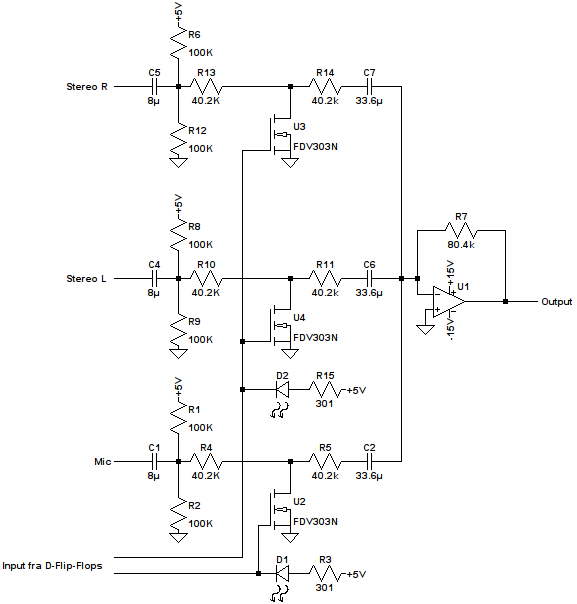
\includegraphics[scale=0.8]{teknisk/indgangsvaelger/simulering/indgangvaelger_ltspice_diagram.png}
\caption{Diagram over det kredsløb der simuleres.}
\label{diagram_simulering}
\end{figure}

\subsubsection*{Forstærkning i kredsløbet}
Fra beregningerne vides det at kredsløbet er designet til at have en forstærkning på 1. Derudover vil signalet efter indgangsvælgeren også være inverteret fordi der bruges en inverterende forstærker til at summere signalerne. Det simulerede signal er vist på figur \ref{indgangsvaelger_input/output}. Simuleringen er lavet ved en transient analyse over 3 ms, med en maksimum timestep på 0,01 µs og en peakspænding på 2 V 1 kHz på indgangen. På figur \ref{indgangsvaelger_input/output} ses det at forstærkningen på 1 ikke helt er opnået, det skyldes at generatoren har en udgangsmodstand på 2,2 k\ohm. Signalet er inverteret som forventet. 
\begin{figure}[h]
\centering
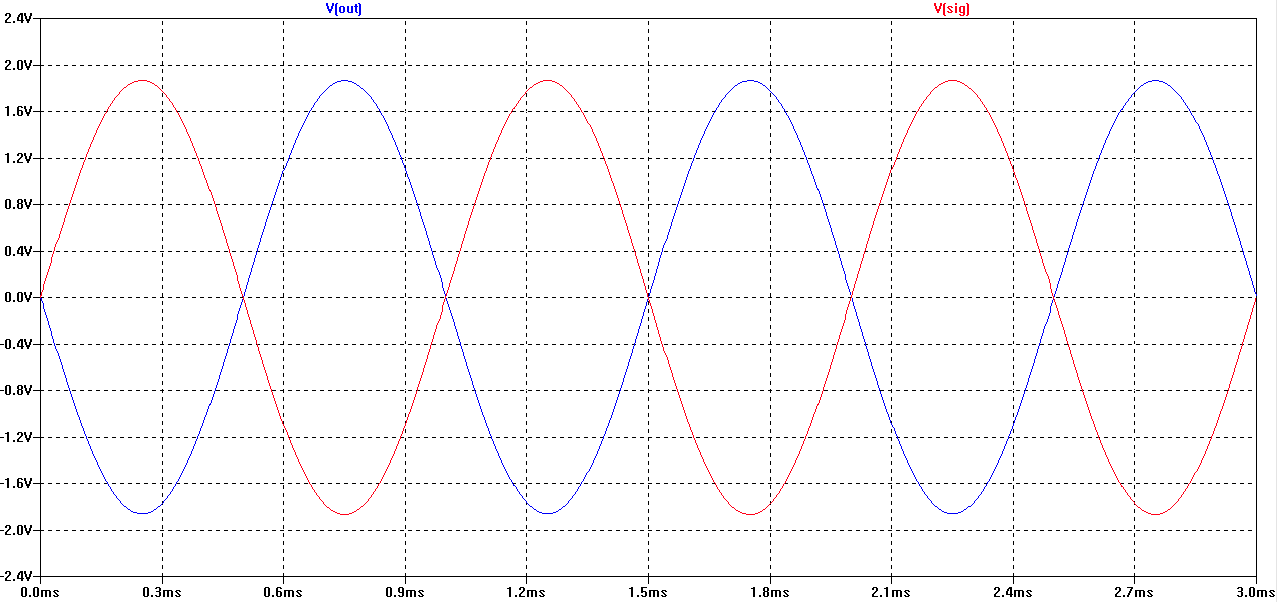
\includegraphics[width=\textwidth]{teknisk/indgangsvaelger/simulering/input_output.png}
\caption{Simuleret forstærkningen igennem indgangsvælgeren, hvor den røde kurve er inputsignalet til indgangsvælgeren og den blå er outputsignalet fra indgangsvælgeren}
\label{indgangsvaelger_input/output}
\end{figure}

\subsubsection*{Frekvenskarakteristik}
På figur \ref{indgangsvaelger_frekvenskarakteristik} er simuleringen af frekvenskarakteristikken vist. Simuleringen er lavet ved en AC-Analyse fra 2 Hz til 200 kHz, og ved at sætte output over input ved 0 V på transistoren. Fra tabel \ref{tab:krav_indgangsvaelger} er der opsat krav om frekvensområdet. På simuleringen ses det at fra 10 kHz til 20 kHz er der en lille afvigelse på ca. 0,06 dB. Afvigelsen skyldes at transistoren der er brugt har en passiv kapacitet, der gør at ved høje frekvenser vil signalet falde af.

\begin{figure}[h]
\centering
\includegraphics[width=\textwidth]{teknisk/indgangsvaelger/simulering/frekvenskarakteristik.png}
\caption{Simuleret frekvens- og fasekarakteristikken for indgangsvælgeren}
\label{indgangsvaelger_frekvenskarakteristik}
\end{figure}

\subsubsection*{Dæmpning af signal}
På figur \ref{indgangsvaelger_daempniing} ses en graf over den simulerede dæmpning i kredsløbet. Simuleringen er lavet ved en AC-Analyse fra 2 Hz til 200 kHz, og ved at sætte output over input ved 5 V på transistoren. Fra kravspecifikationen er der opsat krav om at isoleringen af signaler skal være større end 50 dB, hvilket altså opnåes i simuleringen.
\begin{figure}[h]
\centering
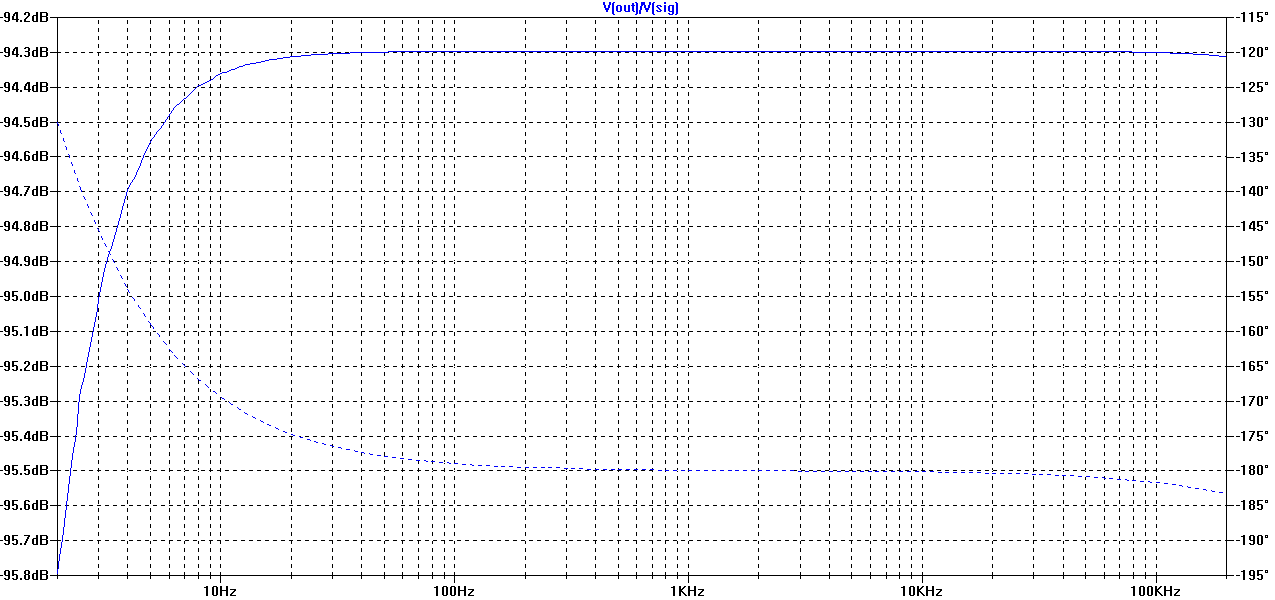
\includegraphics[width=\textwidth]{teknisk/indgangsvaelger/simulering/daempning_af_signal.png}
\caption{Dæmpningsgraden af signalet, når det er slukket.}
\label{indgangsvaelger_daempniing}
\end{figure}
\fixme{Ret den jf. Jans kommentarer}

\subsubsection*{Tænd og sluk af signal}
På figur \ref{indgangsvaelger_taendsluk} er der simuleret at et signal bliver tændt og slukket. Simuleringen er lavet ved en transient analyse over 1,4 s, med en maksimum timestep på 0,1 µs og en peakspænding 2 V ved 100 Hz på indgangen. Først er signalet slukket i 100 ms, dernæst er signalet tændt i 700 ms og til sidst er signalet slukket i 600 ms. Som det ses er signalet når det bliver tændt først oppe på niveau efter det har været tændt i 700 ms. Det skyldes at der er brugt kondensatorer i kredsløbet, hvilket giver en længere indsvingningstid.\fixme{Jesper: Der skal ses på hvad denne graf egentlig betyder}
\begin{figure}[h]
\centering
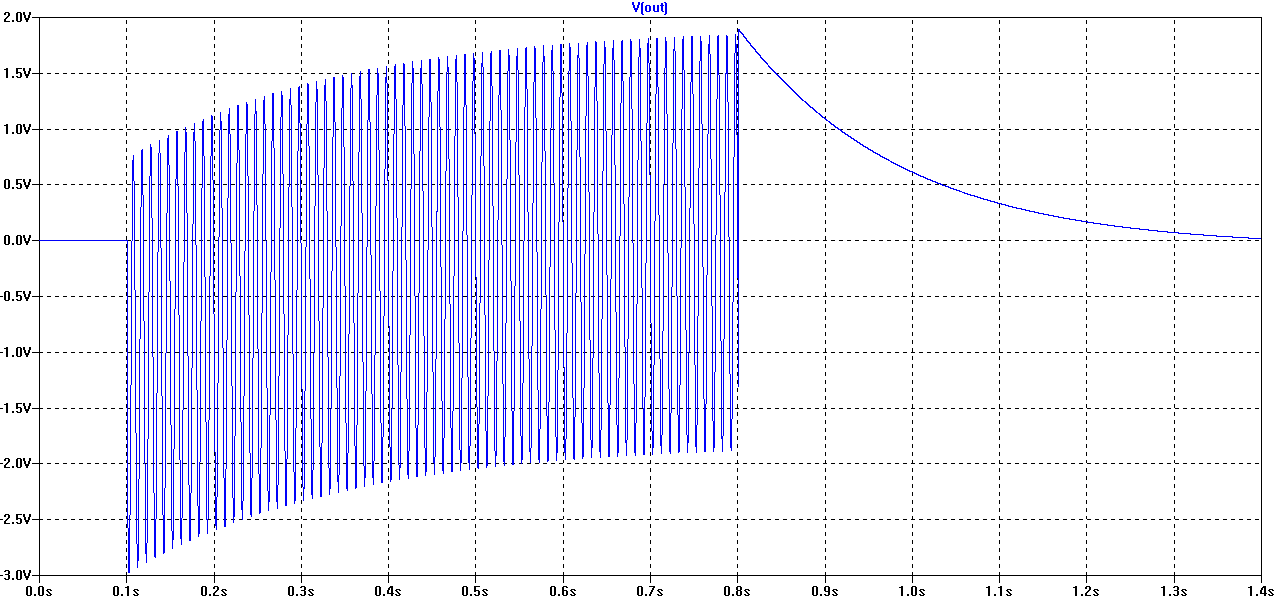
\includegraphics[width=\textwidth]{teknisk/indgangsvaelger/simulering/taend_sluk.png}
\caption{Simulering af at tænde og slukke signalet.}
\label{indgangsvaelger_taendsluk}
\end{figure}

\subsubsection*{THD}
Simuleringen er lavet ved en fourier-analyse og giver en THD på 0,062 \%. Der er dog ikke noget sammenligningsgrundlag fra beregningerne, hvormed der først kan laves udtalelser på denne værdi under accepttesten.

\section{Implementering}
Under konstruktionen af indgangsvælgeren kunne det konstateres at en kondensator ikke umiddelbart var tilgængelig i hverken størrelsesordenen 8$\mu$F eller 33,6$\mu$F. Dette problem blev løst ved at benytte sig af reglen om at hvis to komponenter sidder i parallel kan deres admittans adderes. Admittansen er den reciprokke værdi af resistansen. Da resistansen for en kondensator er givet ved $\frac{1}{s\cdot C}$ bliver admittansen derfor $s\cdot C$. Derfor vil to kondensatorer der sidder i parallel agere som én større kondensator. Derfor blev to 4$\mu$F brugt i stedet for en enkelt 8$\mu$F og en 10$\mu$F og en 22$\mu$F blev benyttet i stedet for en 33.6$\mu$F. Da tolerancen på en elektrolyt kondensator har en tolerance på 20\%\fixme{Kilde: til tolerance på kondensator}  dømmes dette til at være acceptabelt.

\section{Accepttest}
Indgangsimpedansen for alle indgange gav samme resultat ved målingerne. Indgangsimpedansen, for et slukket og et tændt signal, er, som vist i Appendiks \ref{maalejournal_indgangsvaelger}, henholdsvis 22,62 k\ohm~ og 31,56 k\ohm . Da disse begge er over 22 k\ohm~samt stemmer overens med beregningerne, indenfor komponenttolerancerne, er indgangsimpedansen acceptabel.

Frekvensgangen for 200 mV og 2 V inputspænding, er meget éns, derfor tages der kun udgangspunkt i den ene. Det er valgt at konkludere på frekvensgangen for 200 mV, da denne giver det største udsving. En graf over de målte data kan ses på figur \ref{fig:indacc:frek200mv}.
\begin{figure}[h]
\centering
\includegraphics[width=\textwidth]{maalerapporter/indgangsvaelger/Indgangsvlger-mic-200mv-frek.png}
\caption{Målt frekvensgang for mikrofonindgangen på indgangsvælgeren ved 200 mV inputspænding}
\label{fig:indacc:frek200mv}
\end{figure}

Dæmpningen af et tændt signal ved referencefrekvensen, 1 kHz, er i målingen aflæst til 0,034 dB. Den frekvens som afviger mest fra denne værdi er ved 20 kHz, som aflæses til en dæmpning på 0,13 dB. Dette giver en afvigelse på ca. 0,1 dB, hvilket er meget tæt på det simulerede og under det opstillede krav på 0,375 dB. Dette er derfor acceptabelt.

Målingerne viser, på figur \ref{fig:indaccept:slukketmaaling}, at dæmpning ved 1 kHz er på ca. 114 dB. Denne dæmpning er større end det opstillede krav på 50 dB og er derfor accepteret.
\begin{figure}[h]
\centering
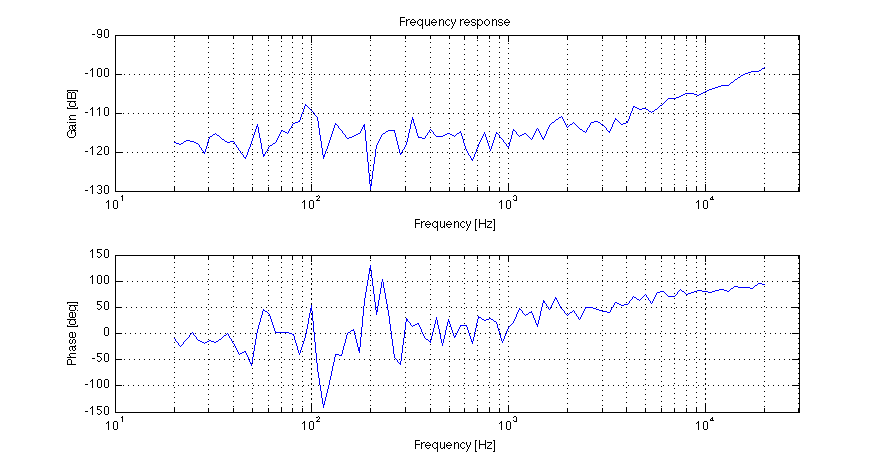
\includegraphics[width=\textwidth]{maalerapporter/indgangsvaelger/Indgangsvlger-mic-2v-slukket-frek.png}
\caption{Frekvensgangen og fasedrejet for mikrofonindgangen for et slukket signal, på indgangsvælgeren ved 2 V. Disse målinger er sandsynligvis støj, da spændingerne er på et meget lavt niveau}
\label{fig:indaccept:slukketmaaling}
\end{figure}	

THD simuleres til 0,062 \% ved en peakspænding på 2 V, ved 1 kHz. Ved en THD måling, illustreret på figur \ref{fig:accind:thd2v}, aflæses THD'en ved 1 kHz til 0,1 \%. 
\begin{figure}[h]
\centering
\includegraphics[width=\textwidth]{maalerapporter/indgangsvaelger/Indgangsvlger-mic-2v-thd.png}
\caption{Målt THD for mikrofonindgangen på indgangsvælgeren ved 2 V inputspænding}
\label{fig:accind:thd2v}
\end{figure}
Det kan dog konkluderes at THD ikke er lav nok. Dette kan delvist løses ved at benytte en anden operationsforstærker, f.eks. OPA27 i stedet for LM324. Det er dog tydeligt, ud fra Appendiks F, at transistorerne ikke afbryder helt, når signalet ikke skal slukkes og at de derfor har en indflydelse. Dette er ikke optimalt og det ville derfor være bedre at benytte en transistor, som afkobler bedre i slukket tilstand.

\begin{table}[h]
\centering
\begin{tabular}{l|r|r}
\hline\hline
Område & Krav & Status \\
\hline\hline
Antal trin i & 4 & \checkmark \\
indgangsvælgeren & \\[4pt]
Indgangsimpedans & > 22 k\ohm & \checkmark \\[4pt]
Frekvensgang & < 0,375 dB ved 20 Hz - 20 kHz, ref. 1 kHz & \checkmark \\
& < 0,75 dB fra 20 Hz til 63 Hz & \checkmark\\
& < 0,75 dB fra 12,5 kHz til 20 kHz & \checkmark\\[4pt]
Dæmpning af slukket & > 50 dB ved 1 kHz & \checkmark \\
indgangssignal & \\
\hline\hline
\end{tabular}
\caption{Oversigt over status af krav til indgangsvælgeren}
\label{tab:krav_indgangsvaelger}
\end{table}

%Volumenkontrol
\chapter{Volumenkontrol}
\label{volumenkontrol}

\section{Design}
\label{volumenkontrol-design}

\begin{figure}[h]
\centering
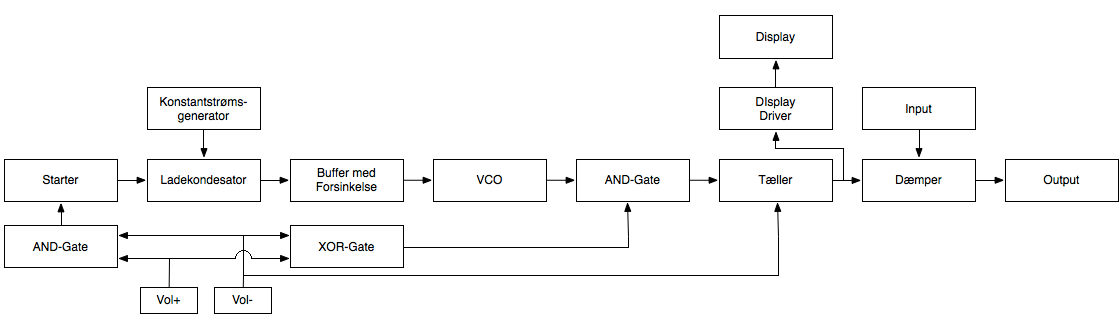
\includegraphics[width=\textwidth]{teknisk/volumenkontrol/blokdiagram.png}
\caption{Blokdiagram over volumenkontrollen}
\label{fig:volumenkontrol_opbygning}
\end{figure}

\section{Simulering}
\label{volumenkontrol-simulering}

\begin{figure}[h]
\centering
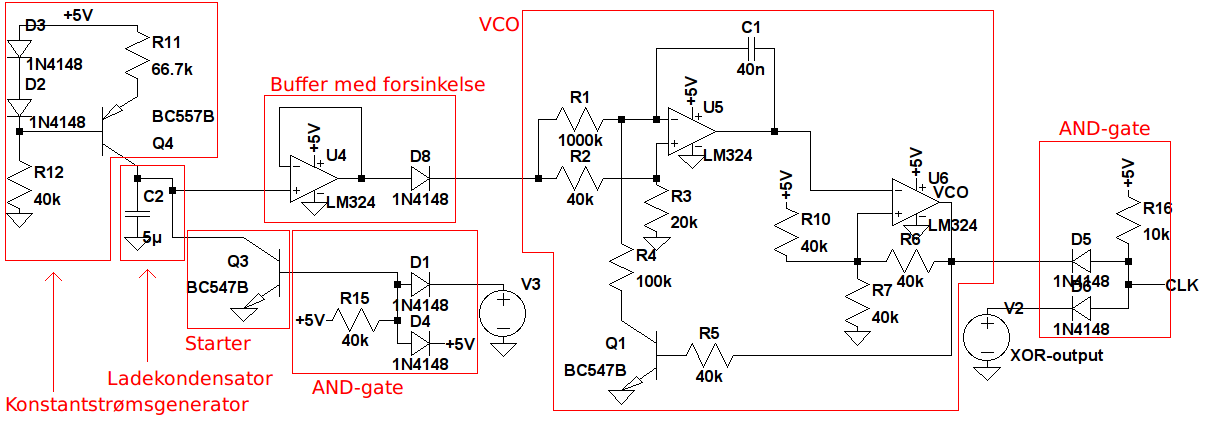
\includegraphics[width=\textwidth]{teknisk/volumenkontrol/diagram.png}
\caption{Diagram over volumenkontrollen}
\label{fig:volumenkontrol_diagram}
\end{figure}

\subsection{Konstantstrømsgenerator}
\label{volumenkontrol-simulering-konstantstroemsgenerator}

Konstantstrømsgeneratorens opgave er at levere en konstant strøm, denne strøm bruges til at oplade en kondensator (ladekondensatoren). Når en kondensator lades med en konstant strøm, vil spændingen over den stige lineært, dette fremgår også af ligning \ref{equ:konstantstroemsgenerator1}.

\begin{equation}
\label{equ:konstantstroemsgenerator1}
V = \frac{I \cdot t}{C}
\end{equation}

Konstantstrømsgeneratoren er designet med udgangs på at der vil være et spændingsfald på 0,5 V over $D_2$, $D_3$, $R_{11}$ og $Q_{4_{BE}}$. I databladet for 1N4148 fremgår det at den vil have en $V_D$ spændingen på 0,5 V ved en $I_F$ strøm på 0,1 mA. Strømmen igennem dioderne er givet ved den strøm, der vil løbe igennem det der kommer efter dem, i dette tilfælde modstanden $R_{12}$. $R_{12}$ er således givet ved ligningen \ref{equ:konstantstroemsgenerator2}.

\begin{equation}
\label{equ:konstantstroemsgenerator2}
R_{12} = \frac{V_{CC} - 2 \cdot V_D}{I_F} = \mathrm{\frac{5~V - 2 \cdot 0,5~V}{0,1~mA} = 40~k\ohm}
\end{equation}

Da der nu ligger en konstant spænding over alle dioderne, kan man se dioden i transistoren som siddende parallelt, med det samme spændingsfald som $D_2$. Dette giver at der findes det samme, konstante, spændingsfald over $D_3$ og $R_{11}$, hvilket giver en konstant strøm gennem $R_{11}$.
Den kondensator som konstantstrømsgeneratoren kaldes ladekondensatoren, denne har en kapacitet på 5 $\mu\mathrm{F}$ og den ønskede oplade tid er 3 s. Kondensatoren oplades fra 0 V til $V_{CC} - V_D$ = 4,5 V, hvor $V_D$ er spændingen over én diode. Udfra disse to ting kan den konstante strøm, $I_{konst}$, nu beregnes, se ligning \ref{equ:konstantstroemsgenerator3}.

\begin{equation}
\label{equ:konstantstroemsgenerator3}
V_{CC} - V_D = \frac{I_{konst} \cdot t}{C} \Rightarrow 4,5~V = \frac{I_{konst} \cdot 3~s}{5~\mu F} \Rightarrow I_{konst} = 7,5~\mu A
\end{equation}

Spændingen over $R_{11}$ er, som tidligere nævnt, 0,5 V og strømmen igennem den er $I_{konst}$, der kan Ohms lov bruges til at beregne modstanden, se ligning \ref{equ:konstantstroemsgenerator4}.

\begin{equation}
\label{equ:konstantstroemsgenerator4}
V_D = R \cdot I_{konst} \Rightarrow 0,5~ V = R \cdot 7,5~\mu A \Rightarrow R = 66,7~k\ohm
\end{equation}

\subsection{Starter}
\label{volumenkontrol-simulering-starter}

Starterens opgave er at holde spændingen over ladekondensatoren på 0 V, når der ikke trykkes på en af volumenknapperne. Dette gøres ved at lede al den strøm som konstantstrømsgeneratoren leverer til stel. Så snart der trykkes på en af volumenknapperne, vil basis på transistoren blive trukket lav, hvilket vil afbryde collector-emitter strømmen. Dette gøres for at sikre at ladekondensatoren er klar til at starte opladningen med det samme.
\subsection{Buffer med forsinkelse}
\label{volumenkontrol-simulering-buffer}

Bufferen sikrer at ladekondensatoren bliver lineært opladet, dette gøres ved ikke at belaste konstantstrømsgeneratoren eller ladekondensatoren. Forsinkelsen laves ved hjælp af en diode. Dioden forsinker signalet ved blot at have et spændingsfald over den, det betyder at spændingen først skal vokse op til minimum en diodespænding, før der kommer en kontrolspænding til VCO'en. Forsinkningen er derfor direkte afhængig af diodespændingen. Dette betyder, at der for at kunne indstille på forsinkelsesperioden skal indsættes en anden diode, med en anden $V_{D}$; eksempelvis en eller flere germaniumsdioder.

\subsection*{VCO}
\label{volumenkontrol-design-vco}

En VCO, Voltage Controlled Oscillator, leverer et konstant signal hvor frekvensen er afhængig af en kontrolspænding. Kontrolspændingen er spændingen over $C_2$, ladekondensatoren, minus én diodespænding. Der er taget udgangspunkt i en VCO fra databladet for en LM324. VCO'en kan deles op i to blokke; én integrator og én schmidt-trigger. Det er udgangen fra schmidt-triggeren der bestemmer hvilken af de to spændinger integrator arbejder udfra. Triggerspændingerne på schmidt-triggeren er givet ved ligning (\ref{equ:vco1}) og (\ref{equ:vco2}). Forsyningsspændingen, $V_{CC}$, er 5 V.

\begin{equation}
\label{equ:vco1}
V_L = \frac{1}{3} \cdot V_{CC} = 1,67~\mathrm{V}
\end{equation}

\begin{equation}
\label{equ:vco2}
V_U = \frac{2}{3} \cdot V_{CC} - 0,5~\mathrm{V} = 2,83~\mathrm{V}
\end{equation}

Frekvensen VCO'en vil svinge med, er givet ved ligning (\ref{equ:vco3}), udtrykket er udledt i appendiks A??.

\begin{equation}
\label{equ:vco3}
f = \frac{1}{\frac{2 \cdot V_{CC} \cdot C \cdot R_1^2}{3 \cdot V_C \cdot (R_1 - R_4)}} = \frac{3 \cdot V_C \cdot (R_1 - R_4)}{2 \cdot V_{CC} \cdot C \cdot (R_1)^2}
\end{equation}

Forholdet mellem høj og lav, duty-cyclen, er givet ved forholdet mellem $R_1$ og $R_4$, i dette tilfælde $\frac{R_4}{R_1} = \frac{40~k\ohm}{80~k\ohm}=0.1$. Dette skyldes at det er disse to modstande $C_1$ op- og aflades igennem. Formlen er udledt i appendiks A??. Grunden til at frekvensen stiger når spændingen stiger, er at opampen altid vil presse sine indgange til at være ens. Da der på plus-indgangen sidder en spændingsdeling, som giver halvdelen af styringsspændingen, vil der ligge det samme på minus-benet. Dette betyder, at spændingsfaldet over $R_1$ altid vil være halvdelen af styringsspændingen. Dette vil betyde at der vil løbe en strøm igennem $R_1$ ind i kondensatoren. Når transistoren leder, vil den lede strømmen, som løber igennem $R_1$ samt den strøm der kommer fra kondensatoren. Når kondensatoren aflader igennem transistoren vil den prøve at trække minus benet ned. Dette prøver op-ampen at undgå ved at øge output spændingen. Hvis man lader denne proces fortsætte uendeligt vil plus- og minus-benet være ens, indtil op-ampen rammer sin maksimale spænding. Herefter vil den ikke være i stand til at regulere spændingen på minus-benet, hvilket vil resultere i at spændingen på minus-benet vil være spændingsdelingen mellem $R_1$ og $R_4$. Dette forhindrer Schmidt-triggeren dog, ved at ændre på hvor strømmen igennem $R_1$ har mulighed for at løbe hen. Når der løber strøm til minus-benet vil dette føre til en spændingstigning. Da op-ampen stadig vil forsøge at holde indgangene éns, vil dette betyde et spændingsfald på outputtet. Det er denne effekt der gør svingningen mulig.

Outputtet fra Schmidt-triggeren er højt, som standard, da outputtet fra integratoren, når denne ikke har en høj nok styringsspænding til at gå i gang, vil være lavt. Dette betyder at AND-gaten der giver signalet videre til tælleren kan give et positivt output, når en knap trykkes ned en enkelt gang. På denne måde vil det være muligt benytte knapperne til at regulere et enkelt niveau op eller ned, samtidig med muligheden for at holde dem inde, og aktivere VCO'en, for at regulere volumeniveauet hurtigere.


%Denne strøm kan kun løbe ind i kondensatoren, hvilket vil oplade denne. Når kondensatoren aflades gennem $R_4$ vil minusbenet gå mod en lavere spænding. For at undgå dette vil op-ampen outputte en højere spænding, for at forsøge at holde begge input på samme spændingsniveau. Kondensatoren blev ved med at aflade, ville op-ampen til sidst nå sit maksimale output. Når dette sker, vil minus benet falde til en spændingsdeling mellem $R_1$ og $R_4$, hvis transistoren $Q_1$ ses som en kortslutning. Dette vil dog ikke ske i praksis, da schmidt-triggeren forhindrer netop dette. 


%I takt med at spændingen stiger over ladekondensatoren vil spændingen over $R_1$ og $R_2$ stige. Dette vil betyde at strømmen ind i kondensatoren, $C_1$ bliver større. Dette forklarer hvordan low-tiden bliver mindre. Kondensatoren vil stadig skulle aflade igennem $R_4$, hvilket umiddelbart ikke lægger op til en kortere høj-tid. Dog vil spændingen over $R_2$ også stige, hvilket gør outputtet fra integratoren højere. Dette vil betyde en lavere spænding over kondensatoren, hvilket vil betyde at den ikke kan lade lige så meget op og den derfor hurtigere kan aflades.
%Hvis V_C stiger vil spændingen på V_+ stige og dermed også V_-. Det vil lave en størrer spænding over R_1 og R_4, og strømmen igennem dem vil så også stige. Hvis kondensatorens kapacitet er konstant og strømmen den op- og aflades med er stigende vil op- og afladetiden falde.
\subsection*{AND-gate}
\label{volumenkontrol-design-and}

De to AND-gates er designet med diskrete komponenter, fremfor en integreret kreds. AND-gaten fungerer ved at holde udgangen høj, når begge indgange er høje. På AND-gaten til venstre på figur \ref{fig:volumenkontrol_diagram}, er et højt udgangsniveau $\sim$0,6 V, dette skyldes at der på udgangen af gaten er en transistors basis-emitter diode til stel. Er blot den ene af indgangene lave, vil den trække udgangen til stel gennem den tilhørende diode, BAT85 \cite{bat85-datablad}. Databladet for dioden beskriver en sammenhæng mellem en diode spænding på 0,24 V og en strøm gennem den på 0,1 mA, dette resultere i en Pull-up modstand beregnet i ligning (\ref{equ:and-gate1}).

\begin{equation}
\label{equ:and-gate1}
V_{CC} - V_D = R_{15} \cdot I_F = 5~\mathrm{V} - 0,24~\mathrm{V} = R_{15} \cdot 0,1~\mathrm{mA} \Rightarrow R_{15} = 47,6~\mathrm{k}\ohm
\end{equation}

Udgangen af AND-gaten vil altså ikke kunne bliver højere end 0,24 V, ved lavt output.

\clearpage
\subsection*{Tæller og displaydriver}
\label{volumenkontrol-design-taeller}

\begin{figure}[h]
\centering
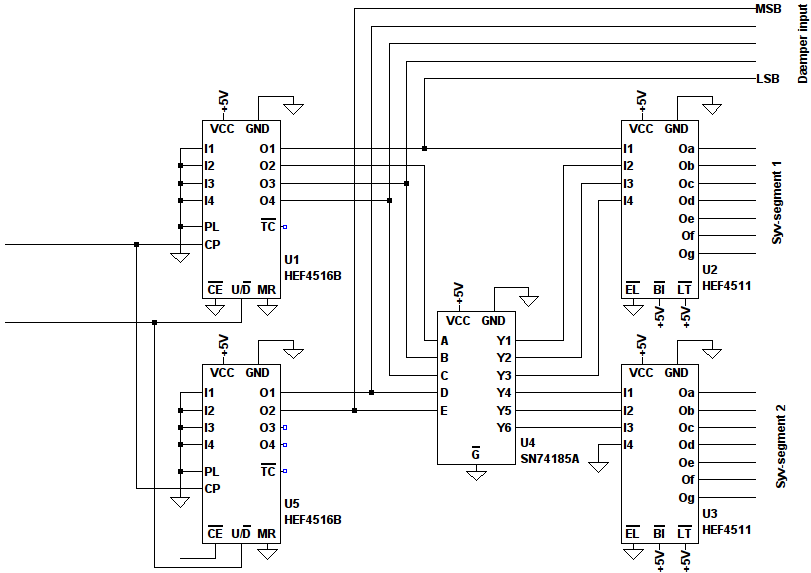
\includegraphics[width=\textwidth]{teknisk/volumenkontrol/taeller.png}
\caption{Diagram over tælleren og displaydriveren}
\label{fig:taeller}
\end{figure}

Tællerens opgave er at holde styr på hvad volumenniveauet er og diagrammet for den er vist på figur \ref{fig:taeller}. Der tælles op eller ned når der trykkes på én af de to volumenknapper. Hvor hurtigt der skal tælles, bestemmes af det AND'ede signal fra VCO'en og XOR-gaten. VCO'en fungerer som en clock på AND-gaten, mens XOR-signalet sørger for, at det kun er den ene knap der holdes nede. Hvis begge knapper holdes nede, vil XOR-signalet være lavt, og der vil intet signal blive sendt til tælleren. Om der skal tælles op eller ned, styres af et signal fra den knap der repræsenterer et ønske om en sænkning i volumeniveau. Hvis denne er nede, som den eneste knap, vil tælleren tælle ned af. Hvis denne ikke er nede, men XOR-signalet stadig er højt, betyder det at den anden knap er nede og tælleren vil derfor tælle op. Tælleren giver et binært output, som danner grundlag for hvad der vises i displayet og hvordan reguleringen af volumen indstilles. Tælleren der benyttes er en 4-bit tæller af typen HEF4516B \cite{hef4516b-datablad}. Da fire bit ikke er nok skal der bruges to tællere.
\fixme{Beregninger be here... or there}

Yderligere skal der også bruges kontrollogik, for at sikre tælleren ikke tæller for højt eller lavt og for at styre den anden tæller. Til at lave et endestop i den laveste ende af tællerens område, lægges alle tællerens output bits sammen i en OR-gate. Dette resultere i et nul, hvis tælleren står på nul. Der skal dog være mulighed for at tælle opad, når tælleren står på nul. Derfor skal UP/$\overline{\mathrm{DN}}$ signalet også med i OR-gaten, udgangssignalet vil nu være lavt når tælleren ikke må tælle nedad. Til at lave endestop i den høje ende, tages der udgangspunkt i en tæller værdi på 50, $110010_\mathrm{b}$. Da dette vil være maks værdien for tælleren er det kun de  udgange der er høje, der er af betydning. Når disse og UP/$\overline{\mathrm{DN}}$ signalet bliver samlet i en NAND-gate vil resultatet kun være lavt når der ikke må tælles højere. Dette signal AND'es sammen med signalet for det lave endstop og CLK signalet, dette bevirker at der ikke kommer CLK signal til de to tællere hvis de har ramt et af endestoppene.

Displaydriveren konverterer signalet fra tælleren til et signal der kan vises på de to 7-segment displays. Der konverteres fra tællerens binære output til BCD, Binary-coded decimal, for så at konvertere det til et signal 7-segment displaysne kan vise. Der benyttes en SN74185A \cite{sn74185a-datablad} til konverteringen fra binær til BCD. Fordelen ved at konvertere til BCD først er at denne konvertering også deler det binære tal op i to, en'ere og ti'ere. Disse to binære tal sendes igennem en 7-segmentsdriver, HEF4511 \cite{hef4511-datablad}, for at få et output der fungerer med 7-segmenterne. Displaydriveren er også vist på figur \ref{fig:taeller}.

\subsection*{Display}
\label{volumenkontrol-design-display}
Indstillingen af volumenkontrollen vises på to 7-segmenter. Dette er valgt, fordi disse er enkle at styre med simple kredsløb og det derfor ikke er nødvendigt med en microcontroller for at styre dem, som tilfældet havde været, hvis et LCD-display i stedet var blevet benyttet.

\subsection*{Dæmper}
\label{volumenkontrol-design-daemper}
Dæmperen er en en analog attenuator, som er sammensat af to sæt modstandsattenuatore, hver efterfulgt af en buffer. Dæmpningen indstilles ved at ændre, hvor signalet tages ud af de to modstandsattenuatore, ved brug af en analog multiplekser. Den første attenuator består af syv modstande, hvor der er en dæmpning på 8 dB mellem hver modstand. Den anden attenuatorer består af otte modstande, hvor der er en dæmpning på 1 dB mellem hver modstand. Det er således muligt at kombinere de to attenuatorer til at dæmpe signalet mellem 0 og 55 dB, med et interval på 1 dB. Diagrammet er afbilledet på figur \ref{fig:volumenkontrol_daemper} og modstandene derpå er beregnet i Appendiks C??.

\begin{figure}[h]
\centering
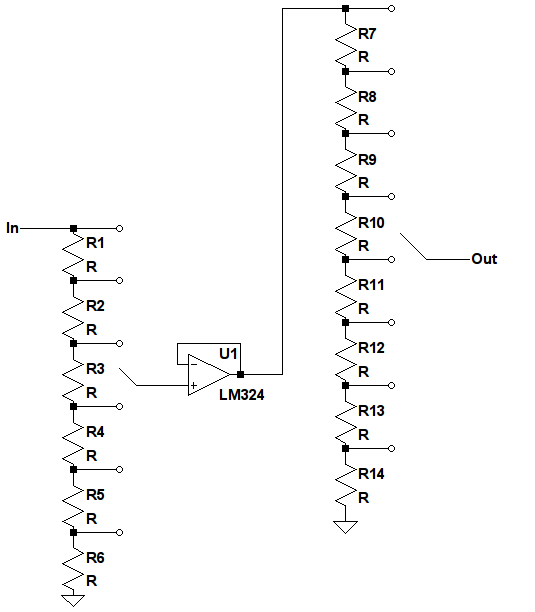
\includegraphics[width=\textwidth]{teknisk/volumenkontrol/daemper.png}
\caption{Diagram over dæmperen}
\label{fig:volumenkontrol_daemper}
\end{figure}

\clearpage
\section{Simulering}
\label{volumenkontrol-simulering}

På figur \ref{fig:volumenkontrol-diagram} er vist diagrammet, med komponent værdier, over volumenkontrollen til og med signalet til tælleren.

\begin{figure}[h]
\centering
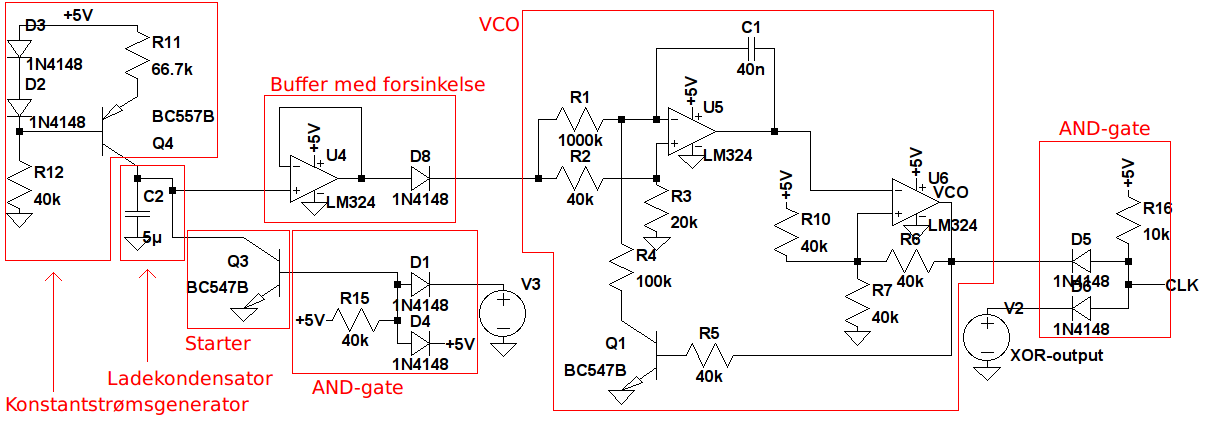
\includegraphics[width=\textwidth]{teknisk/volumenkontrol/diagram.png}
\caption{Diagram over volumenkontrollen}
\label{fig:volumenkontrol-diagram}
\end{figure}

På figur \ref{fig:vco-signal} ses resultatet af at påtrykke en konstant spænding på VCO'en. Dette resulterer i udgangen på integratoren, den blå kurve, svinger mellem schmitt-triggerens to niveauer med en fastdefineret frekvens. Det kan ses at plusindgangen på schmitt-triggeren, den røde kurve, er høj når integratorens udgang er opadgående og lav når den er nedadgående. 

\begin{figure}[h]
\centering
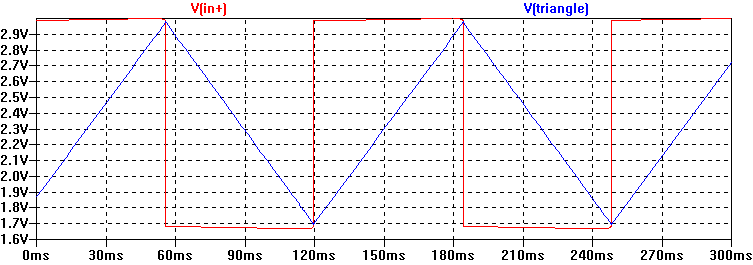
\includegraphics[width=\textwidth]{teknisk/volumenkontrol/vco-signal.png}
\caption{Integratorens udgang og plusindgangen på schmitt-triggeren}
\label{fig:vco-signal}
\end{figure}

Figur \ref{fig:stresstest} viser hvordan volumenkontrollen fungerer, når man trykker på en knap. Den blå graf, V(knap), viser knappens tilstand; når den er lav, er knappen trykket ned. Den lyseblå, V(clk) viser outputtet til clocken. Clocken på tælleren er flankestyret, hvilket vil sige, at der kun vil blive flyttet et trin, hver gang den lyseblå, V(clk) går fra lav til høj. Når knappen holdes nede, kan man se at kontrolspændingen, V(vc), stiger. Dette vil få spændingen på udgangen af integratoren, V(triangle), til at stige, indtil den rammer den høje trigger-spænding. Herefter vil spændingen falde igen, og oscillere hurtigere og hurtigere, i takt med at kontrolspændingen stiger. Ca. 3 sekunder efter at knappen trykkes ned, rammer kontrolspændingen sit max, som udregnet. Her vil udgangen på integratoren, og derfor også schmitt-triggeren, svinge med en frekvens på ca. 10 Hz.

\begin{figure}[h]
\centering
\includegraphics[width=\textwidth]{teknisk/volumenkontrol/stress-test.png}
\caption{Simulering af at trykke på og holde en knap nede.}
\label{fig:stresstest}
\end{figure}

På figur \ref{fig:konstantstroem} ses en simulering af konstantstrøms generatoren. Det er tydeligt at se, at konstantstrømsgeneratoren genererer en konstant strøm, Ic(Q4), indtil den ikke har et sted at løbe hen. Dette sker når kondensatoren er ladet op. Det er desuden tydeligt at se at kondensatoren, V(c2), bliver opladet lineært, med det samme knappen, V(knap), bliver trykket ned. 

\begin{figure}[h]
\centering
\includegraphics[width=\textwidth]{teknisk/volumenkontrol/konstantstroem.png}
\caption{Simulering af konstanstrømsgeneratoren}
\label{fig:konstantstroem}
\end{figure}
\section{Implementering}
Under implementering af volumen kontrollen, kunne der konkluderes at der var en række problemer med designet. Det kunne konkluderes at spændingen på udgangen af at LM324 ikke blev trukket helt lav, efter den sidste AND-gate blev monteret. Dette betød at transistoren åbnede konstant, hvilket umuliggjorde svingning. Efter at have undersøgt databladet for LM324, blevet det konstateret at den kun kan tage 50 $\mu$A, ind i udgangen, ved en meget lav spænding. Derfor blev det besluttet at skifte $R_{16}$ på 48,5~k$\ohm$ ud med en modstand på 487~k$\ohm$ , for at sænke strømmenmed en faktor 10, hvilket både vil give et lavere spændingsfald over dioden samt sørge for det løber en mindre strøm ind i opampen. Dette løste problemet. Der blev også diskuteret at benytte en buffer i stedet, men dette blev nedstemt, da dette ville betyde en større ændring, end at skifte en modstand.

Det kunne yderligere konstateres, at der findes en fejl i designet, der dog er yderst sjælden. Hvis man slipper en knap mens spændingen på udgangen af integratoren er nedadgående, vil Schmidt-triggeren være lav, hvilket betyder at transistoren vil være lukket. Da signalet fra schmidttriggeren AND'es sammen med signalet fra XOR-gaten, vil det er ikke være muligt at få et clock output til tælleren. Der kan derfor argumenteres for en høj dutycycle, for at formindske chancen for at slippe knappen mens schmidt-triggeren er lav. Da tælleren alligevel er triggered på opadgående flanker, vil der kun komme ét output signal pr. periode. For at komme ud af denne tilstand, kan en knap holdes nede indtil ladekondensatoren kommer over diodespændingen så der igen kommer en input spænding på integratoren, hvilket vil starte svingningen igen. 
For at modvirke det, sættes en modstand, $R_{\mathrm{stor}}$, fra minusbenet på integratoren til forsyningsspændingen. Dette vil betyde at kondensatoren kan oplade, hvilket betyder at minus-indgangen på schmidt-triggeren vil gå lav. Når minus indgangen er lavere end plus indgangen, vil udgangen gå høj, hvilket vil åbne transistoren. Når transistoren er åben vil der være en spændingsdeling imellem $R_{\mathrm{stor}}$ og $R_4$ parallelt med $R_1$, $R_2$ og $R_3$ i serie. Der vil ligge en meget lille spænding på minus indgangen, da størstedelen af spændingen vil ligge over den største modstand. Det vigtige er dog, at spændingen på plus-indgangen er endnu mindre. Dette vil tvinge udgangen på op-ampen nedad. Denne opstilling vil sørge for at outputtet på integratoren er lavt, hvilket vil sørge for at schmidttriggeren vil være høj. Hvis schmidttriggerens output ikke havde styret transistoren ville integratoren stadig outputte lavt, da der så bare vil sidde en spændingsdeler bestående af $R_{\mathrm{stor}}$, $R_1$, $R_2$ og $R_3$.
For at denne store modstand $R_{\mathrm{stor}}$ ikke skal have noget at sige for svingningsforløbet er den valgt til at være 100 gange større end $R_1$; altså 8 M$\ohm$
\section{Accepttest}
\label{volumenkontrol-accepttest}
Det kan konkluderes at VCO'en fungerer som simuleret, og denne må derfor ses som en succes. Tælleren fungerer derimod ikke tilfredsstillende. Den kan i enkelte tilfælde tælle op til 51. Årsagen til fejlen er ikke lokaliseret. Desuden tæller den i nogle tilfælde op, selvom den burde tælle ned. Dette er dog ikke tilfældet, hvis knappen holdes inde. Årsagen til denne fejl er heller ikke lokaliseret. Tælleren ses derfor som ikke at leve op til kravet. Displayet samt displaydriverne fungerer og viser de rigtige tal ud fra det input de får.

Dæmpningen af signalet fungerer som forventet, se Appendiks \ref{maalevolumenkontrol}. THD-målingerne i volumenkontrol viser at den, ved højeste volumen, er under 0,01\% på sit højeste, som set på figur \ref{fig:accvold:thd0}. Dette accepteres, da dette er lavt i forhold til de 1\%, som er maksimum for hele systemet. 
\begin{figure}[h]
\centering
\includegraphics[width=\textwidth]{maalerapporter/volumenkontrol/2Vniveau0-thd.png}
\caption{THD for volumenkontrollen ved fuldt signal}
\label{fig:accvold:thd0}
\end{figure}

Der findes ved måling, at volumenkontrollen, uden dæmpning, forstærker 0,0027 dB ved 1 kHz. Dette sammenlignes med 0,0021 dB 20 Hz og -0,0015 dB ved 20 kHz. Dette giver en maksimalt afvigelse fra referencefrekvens 1 kHz på 0,0042 dB. Dæmpningsdelen af volumenkontrollen er derfor accepteret.
\begin{figure}[h]
\centering
\includegraphics[width=\textwidth]{maalerapporter/volumenkontrol/2Vniveau0-frek.png}
\caption{Frekvensgang for volumenkontrollen ved fuldt signal}
\label{fig:accvold:frek0}
\end{figure}


\begin{table}[h]
\centering
\begin{tabular}{l|r|r}
\hline\hline
Område & Krav & Status \\
\hline\hline
Frekvensgang & $\pm$ 0,375 dB ved 20 Hz - 20 kHz, ref. 1 kHz & \checkmark \\
& $\pm$ 0,75 dB fra 20 Hz til 63 Hz & \checkmark \\
& $\pm$ 0,75 dB fra 12,5 kHz til 20 kHz & \checkmark \\[4pt]
Dæmpningsområde i & 0 - 50 dB ved 1 kHz & \checkmark \\
volumenkontrol && \\[4pt]
Styring af volumen- & Digital & $\mathcal{X}$ \\
kontrol && \\[4pt]
Antal niveauer i & 51 & $\mathcal{X}$ \\
volumenkontrollen && \\[4pt]
Dæmpning per & 1 dB & \checkmark \\
niveau && \\[4pt]
Input fra brugeren & To trykknapper & \checkmark \\[4pt]
Output til brugeren & To 7-segmenter & \checkmark \\
\hline\hline
\end{tabular}
\caption{Oversigt over status af krav til volumenkontrollen}
\label{tab:krav_volumenkontrol}
\end{table}


%Effektforstærker
\chapter{Effektforstærker}
\label{effektforstaerker}
Formålet med en effektforstærker er, som nævnt i kapitel \ref{systemopbygning}, at levere en strømforstærkning der gør det muligt at afsætte den ønskede effekt i belastningsmodstanden. Dette skal ske uden at der afsættes en stor effekt i selve effektforstærkeren, altså uden den bliver opvarmet unødigt, da denne effekt vil være spild. Effektforstærkeren skal desuden levere denne strømforstærkning uden signalet forvrænges mere end tilladt. \\
Alle kravene der er stillet til effektforstærkeren er opstillet i tabel \ref{tab:krav_effektforstaerker}.

\begin{table}[h]
\centering
\begin{tabular}{l|r}
\hline\hline
Område & Krav \\
\hline\hline
Klasse & AB \\[4pt]
Nyttevirkning & > 25 \%  \\[4pt]
Forvrængning & < 0,5 \% \\[4pt]
Udgangseffekt & > 20 W ved 2 V input \\[4pt]
Frekvensgang & $\pm$ 0,375 dB ved 20 Hz - 20 kHz, ref. 1 kHz \\
& $\pm$ 0,75 dB fra 20 Hz til 63 Hz \\
& $\pm$ 0,75 dB fra 12,5 kHz til 20 kHz \\[4pt]
Belastningsimpedans & 8 \ohm \\[4pt]
Udgangssignaltype & Mono \\[4pt]
Kortslutningsstrøm (peak) & 3 A \\
\hline\hline
\end{tabular}
\caption{Krav til effektforstærkeren}
\label{tab:krav_effektforstaerker}
\end{table}

\section{Design}
\subsection{Strømforstærker}
\label{effekt_stroemforstaerker}
Strømforstærkeren opbygges som vist på figur \ref{fig:blokdiagram-stroem}. Dog vil konstantstrømsgeneratoren blive bygget i diskret elektronik. Der er valgt at der benyttes en BDX33B og en BDX34B \cite{bdx33-34-datablad} som udgangstransistorer. Dette er darlingtontransistorer, som er valgt da de har en $h_{\mathrm{FE}}$ på minimum 750 og kan klare en $I_C$ på op til 10 A. Desuden er de let tilgængelige til projektet.

\begin{figure}[h]
\centering
\includegraphics[scale=0.4]{teknisk/effektforstaerker/blokdiagram-stroemforstaerker.png}
\caption{Diagram over strømforstærkeren}
\label{fig:blokdiagram-stroem}
\end{figure}

Som vist, i afsnit \ref{valg_kortslutningssikring}, skal der igennem $R_{\mathrm{load}}$ løbe en $I_{\mathrm{peak}}$ på 2,24 A for at opnå en udgangseffekt på 20 W. Dette betyder desuden, som vist i udregningen i formel \ref{equ:vpeak}, at der skal være en $V_{\mathrm{peak}}$ på 17,9 V over belastningen for at afsætte 20 W. 

\begin{equation}
\label{equ:vpeak}
V_{\mathrm{peak}} = I_{\mathrm{peak}} \cdot R_{\mathrm{load}} = \mathrm{2,24~A \cdot 8~\ohm = 17,9~V}
\end{equation}

Ideelt vil en spændingsforsyning på 18 V altså være tilstrækkelig, dog er der rent praktisk behov for en større. Da de valgte darlingtontransistorer har en $V_{\mathrm{BE}}$ på op til 2,5 V, vælges forsyningsspændingen til $\pm$23 V, hvormed der også er plads til et spændingsfald over $R_E$ og en transistor i konstantstrømsgeneratoren.

\subsubsection*{Termiske forhold}
Størrelsen af $R_E$ bestemmes med udgangspunkt i at den skal skabe termisk stabilitet og til bestemmelsen af denne startes der derfor med at kigge på et termisk ækvivalentdiagram for de valgte darlingtontransistorer og de tilgængelige køleplader \cite{koeleplade-datablad}. 

\begin{figure}[h]
\centering
\includegraphics[scale=0.2]{teknisk/effektforstaerker/termisk_ekvivalentdiagram.png}
\caption{Termisk ækvivalentdiagram for udgangstransistorerne}
\label{fig:term-dia}
\end{figure}

På figur \ref{fig:term-dia} ses ækvivalentdiagrammet, hvor; temperatur er spænding, effekt er strøm og termisk modstand er modstand. Flere af komponenterne har samme benævnelser, da de også antager samme værdier og da der under udregningerne dermed ikke vil blive set på dem enkeltvis.\\
Størrelsen af $P_D$ er effekten afsat i en enkelt udgangstransistor og er givet ved udregningen i formel (\ref{equ:pd}) \cite{ael-mm19}. Denne formel er ganske vist givet for et klasse B udgangstrin, men den er også gældende for et klasse AB udgangstrin, da hvilestrømmem i et klasse AB udgangstrin kun er betydeligt forskellig fra nul i perioden, hvor der er et skifte i hvilken transistor, som er aktiv \cite{klasse-ab}.

\begin{equation}
\label{equ:pd}
P_D = \frac{1}{\pi^2} \cdot \frac{(V_{CC})^2}{R_{\mathrm{load}}} = \frac{1}{\pi^2} \cdot \frac{(23~\mathrm{V})^2}{8~\ohm} = 6,7~\mathrm{W}
\end{equation}

Fra darlingtontransistorernes datablad haves $R_{\mathrm{jc}} = 1,78~\tfrac{\celsius}{\mathrm{W}}$ og $T_{\mathrm{j,max}} = 150~\celsius$. Databladet for kølepladen giver $R_{\mathrm{cs}} = 1,4~\tfrac{\celsius}{\mathrm{W}}$ når der anvendes kølepasta. Fra DIN45500 \cite{DIN45500} fåes at HiFi-forstærkeren skal kunne holde til en omgivelsestemperatur på 35~\celsius, hvilket er $T_a$ i ækvivalentet. Udfra dette opstilles, ved simpel kredsløbsteori på ækvivalentkredsløbet på figur \ref{fig:term-dia}, formel (\ref{equ:tjmax}) til beregning af $R_{\mathrm{sa}}$ ved $T_j$  på sin maksimale værdi. 

\begin{equation}
\label{equ:tjmax}
T_j = T_a + P_D \cdot (R_{\mathrm{jc}} + R_{\mathrm{cs}} + 2 \cdot R_{\mathrm{sa}})
\end{equation}

Desuden opstilles udfra sikkerhedshensyn et krav om at kølepladen maksimalt må blive 40~\celsius, hvorved bestemmelse af $R_{\mathrm{sa}}$ også kan foregå ved brug af formel (\ref{equ:smax}). 

\begin{equation}
\label{equ:smax}
40~\celsius = 2 \cdot P_D \cdot R_{\mathrm{sa}}
\end{equation}

Det ses at formel (\ref{equ:smax}) bliver den afgørende betingelse og at $R_{\mathrm{sa}}$ maksimalt må være $2,99~\tfrac{\celsius}{\mathrm{W}}$. I databladet for kølepladen ses at en $R_{\mathrm{sa}}$ på $2,9~\tfrac{\celsius}{\mathrm{W}}$ kan opnåes ved en køleplade på 110 mm, hvilket derfor vælges. Størrelsen af $R_E$ kan nu bestemmes ved formel (\ref{equ:rebestem}) \cite{ael-mm19-ole-mod}% \fixme{kilde: Jan Mikkelsen, mm19, modificeret af Ole Kiel Jensen}
, hvor $K = - 2~\tfrac{\mathrm{mV}}{\celsius}$, $V_{CC} = 23$ V, $V_T = 26$ mV og $I_C = 2,24$ A.

\begin{equation}
\label{equ:rebestem}
R_E = - 2 \cdot K \cdot V_{CC} \cdot (R_{\mathrm{jc}} + R_{\mathrm{cs}} + R_{\mathrm{sa}}) - \frac{2 \cdot V_T}{I_C} = 536~\mathrm{m}\ohm
\end{equation}

\subsubsection*{Simulering af termiske forhold}

På figur \ref{fig:term-runaway} er vist en graf over effekten som bliver afsat i en af udgangstransistorerne, når der på dennes emitter sidder den beregnede $R_E$. Den lige turkis linie viser hvilken effekt den samlede køling er i stand til at lede væk, når systemet står et sted hvor omgivelsestemperaturen er 35~\celsius. Den lige grønne linie viser hvilken effekt den samlede køling er i stand til at lede væk, når systemet står et sted hvor omgivelsestemperaturen er 25~\celsius. Systemet vil, når der ikke er noget signal på indgangen, opnå en hviletemperatur svarende til skæringen mellem effektkurven for darlingtontransistoren og $"$kølingslinien$"$, altså lige over 75~\celsius~ved en omgivelsestemperatur på 35~\celsius. Havde systemet ikke indeholdt en $R_E$, eller havde denne været mindre, ville effektkurven for darlingtontransistoren ligge højere, hvormed systemet ville opnå en højere hviletemperatur. 

\begin{figure}[h]
\centering
\includegraphics[width=\textwidth]{teknisk/effektforstaerker/term-runaway.png}
\caption{Graf over termiske forhold med $R_E$ og 110 mm køleplade}
\label{fig:term-runaway}
\end{figure}

Som et forsøg på at forbedre situationen beskrevet på figur \ref{fig:term-runaway}, er der på figur \ref{fig:term-runaway1} vist samme kurver, men med en køleplade på 150 mm monteret i stedet. 

\begin{figure}[h]
\centering
\includegraphics[width=\textwidth]{teknisk/effektforstaerker/term-runaway1.png}
\caption{Graf over termiske forhold med $R_E$ og 150 mm køleplade}
\label{fig:term-runaway1}
\end{figure}

Ved en omgivelsestemperatur på 35~\celsius~ betyder denne ændring, at darlingtontransistoren vil opnå en hviletemperatur som er over 10~\celsius~ lavere, hvilket derfor er at foretrække. Til at lave opstillingerne på figur \ref{fig:term-runaway} og \ref{fig:term-runaway1} er der antaget en hvilestrøm gennem transistoren på 45 mA. Hvilestrømmens størrelse er antaget ud fra 2 \% af peakstrømmen på udgangen, som i eksempel 13.5 i Sedra-Smith \cite{sedra-smith}.%\fixme{sedra smith}


\subsubsection*{$V_\mathrm{BE}$-multiplier}

\begin{figure}[h]
\centering
\includegraphics[scale=.4]{teknisk/effektforstaerker/vbemultiplieropbygning.png}
\caption{Strømforstærkertrinnet med markering af $V_\mathrm{be}$-multiplieren}
\label{fig:vbemulti}
\end{figure}


For at opnå en klasse AB forstærkers karakteristika skal potentialet på basis af darlingtontransistorerne hæves således det ikke er audiosignalet der skal generere den nødvendige basis-emitter-spænding for at darlingtontransistorerne åbner. Hvis ikke potentialet hæves nok vil audiosignalet blive udsat for crossoverforvrængning idet en del af signalets spændning omkring 0 V ikke vil blive overført til højtaleren. Det korrekte potentiale på basis af U1 og U2 opnås ved hjælp af en $V_\mathrm{BE}$-multiplier, hvis funktion er at opretholde et spændingsfald, $V_{BB}$, over Q1, vist på figur \ref{fig:vbemulti}. Ideelt set skal collector-emitter-spændingsfaldet over Q1 være præcis to darlington basis-emitter-spændinger, således at U1 og U2 vil åbne så snart spændingen på basis ændredes. Det anses dog ikke for at være muligt at designe kredsløbet så præcist, blandt andet på grund af tolerancerne i darlington transistorerne, som er relativt store. Derfor designes $V_\mathrm{be}$-multiplieren således at spændingsfaldet over Q1 gør at transistorerne U1 og U2 trækker en relativt lille hvilestrøm når audioinputtet er 0 V. Dermed er der sikret at U1 og U2 er åbne og at audiosignalet ikke bliver udsat for crossoverforvrængning. 


Hvilestrømmen er antaget til 45 mA i afsnittet om termiske forhold. Til Q1 benyttes en BC547B transistor, grundet at det er hvad der er til rådighed. Da der ikke er opgivet en basis-emitterspænding for darlingtontransistorerne ved en collectorstrøm på 45 mA i databladet \cite{bdx33-34-datablad} er den fundet ved hjælp af LTspice og transistorernes spicemodel. Basis-emitterspændingen blev simuleret til 1,25 V. I ligning (\ref{eq:vbbberegning}) bestemmes $V_{BB}$, som er spændingen over $V_\mathrm{BE}$-multiplieren.

\begin{equation}
V_{BB} =2 \cdot 1,25~\mathrm{V} = 2,5~\mathrm{V}
\label{eq:vbbberegning}
\end{equation}

For at opnå et spændingsfald over $V_\mathrm{BE}$-multiplieren skal der løbe en strøm. For at have kontrol over hvilken strøm der løber gennem $V_\mathrm{BE}$-multiplieren leveres denne strøm,  $I_\mathrm{bias}$, af en konstantstrømsgenerator. Generatoren er koblet på $V_\mathrm{BE}$-multiplieren som vist på figur \ref{fig:vbemulti}. Biasstrømmen skal både generere et spændingsfald over $V_\mathrm{BE}$-multiplieren og levere tilstrækkeligt basisstrøm til darlington transistorerne, således at de, ved maksimal spændingssving, ikke begrænses af $I_\mathrm{bias}$. Da der ikke vil være maksimalt signalsving på begge transistorer simultant vil der dermed kun være behov for at levere maksimal basisstrøm til én transistor af gangen. Da collectorstrømmen, $I_C$, i darlingtontransistorerne ved maksimalt signaludsving vides at være 2,24 A kan den maksimale basistrøm, $I_b$, beregnes, da der gælder at $I_b = \frac{I_C}{h_\mathrm{fe}}$. Den maksimale basisstrøm beregnes for en minimumtransistor til at være 3 mA. For at være sikker på at levere tilstrækkeligt strøm vælges $I_\mathrm{bias}$ til at være 6 mA, hvilket giver en minimumstrøm i $V_\mathrm{BE}$-multiplieren på 3 mA. Strømmen i modstandene, $R_7$ og $R_8$, ønskes at være mindre end strømmen Q1,  $I_\mathrm{c,Q1}$. Derfor vælges det at strømmen i modstandene,  $I_R$, skal være 10 gange mindre end $I_\mathrm{C,Q1}$. Dermed bliver $I_R = 0,5$ mA og $I_\mathrm{C,Q1} = 5,5$ mA.

Spændingsfaldet over $R_8$ skal være lig basis-emitterspænding for Q1 ved en collectorstrøm på 5,5 mA. Da der i databladet for en BC547B er angivet en maksimal værdi for basis-emitterspændingen på 0,7 V ved en collectorstrøm på 2 mA og 0,72 V ved en collectorstrøm på 10 mA vælges basis-emitterspændingen til at være 0,7 V. I ligning (\ref{eq:r8beregning}) beregnes $R_8$.

\begin{equation}
R_8 = \frac{V_\mathrm{BE,Q1}}{I_R} = 1,28~\mathrm{k}\ohm
\label{eq:r8beregning}
\end{equation}

Da der skal være et spændingsfald over $V_\mathrm{BE}$-multiplieren, og dermed de to modstande, på 2,5 V kan den samlede modstand $R_7$ og $R_8$ skal repræsentere beregnes hvorefter værdien af $R_7$ kan bestemmes som værende den resterende modstand når $R_8$ er trukket fra.

\begin{equation}
R_7 = \frac{V_{BB}}{I_R} - R_8 = 3,3~\mathrm{k}\ohm
\label{eq:r7beregning}
\end{equation}

En DC-analyse-simulering i LTspice viser at hvilestrømmen i strømforstærkeren bliver 55 mA. Dette passer ikke overens med beregningerne. Dog vil $V_\mathrm{BE}$-multiplieren ikke være korrekt dimensioneret hvis strømforstærkeren forsøges bygget med diskrete komponenter da tolerancerne for darlingtontransistorerne er relativt store. Derfor vil der blive indsat et potentiometer på 5 k\ohm~i stedet for $R_8$ hvorved spændingen over $V_\mathrm{BE}$-multiplieren kan gå ned til 1,16 V da sammenhængen mellem Q1's basis-emitterspænding, $R_7$ og $R_8$ er giver ved ligning (\ref{eq:vbemultipliersammenhaeng}).

\begin{equation}
V_{BB}=V_\mathrm{BE,Q1} \cdot \left( \frac{R_7}{R_8} \right)
\label{eq:vbemultipliersammenhaeng}
\end{equation}

Med potentiometeret er det dermed muligt at justere $V_{BB}$ og dermed også hvilestrømmen der løber i darlingtontransistorerne. Under implementeringen justeres potentiometeret således at hvilestrømmen stemmer overens med den beregnede.

\subsubsection*{Konstantstrømsgenerator}
Konstantstrømsgeneratorens opgave er at levere en konstant strøm. Denne strøm bruges til $V_\mathrm{BE}$-multiplieren og til spændingsforstærkeren. Som beregnet ved beregning af $V_{\mathrm{BE}}$-multiplieren skal konstantstrømsgeneratoren levere 6 mA. Opbygningen der er valgt til konstansstrømsgereratoren er afbildet på figur \ref{konstantstroemsgenerator_model}.

\begin{figure}[h]
\centering
\includegraphics[scale=0.35]{teknisk/effektforstaerker/stoemgenerator.png}
\caption{Diagram der viser opbygningen af konstantstrømsgeneratoren.}
\label{konstantstroemsgenerator_model}
\end{figure}

Til konstantstrømsgeneratoren er der valgt at anvende en BC547B som transistor og en 1N4148 som diode. BC547B har en $V_\mathrm{BE}$ spænding på maksimum 720 mV \cite{bc547b-datablad}. Deraf designes det således at der er et spændingsfald på 720 mV over $D_1$, $D_2$, $R_{\mathrm{11}}$ og $Q_{9_\mathrm{BE}}$. I databladet for 1N4148 \cite{1n4148-datablad} fremgår det at den  ved en $I_F$ strøm på 8 mA har en $V_D$ spændingen på 720 mV. Strømmen igennem dioderne er givet ved hvor stor en strøm der løber igennem modstanden $R_{\mathrm{10}}$, ved den antagelse at der ses bort fra strømmen der løber ind i basen på $Q_9$. $R_{\mathrm{10}}$ er således givet ved ligning (\ref{equ:stroemgenerator_effektforstaerker1}).

\begin{equation}
\label{equ:stroemgenerator_effektforstaerker1}
R_{\mathrm{10}} = \frac{V_{CC} - 2 \cdot V_D}{I_F} = \mathrm{\frac{23~\mathrm{V} - 2 \cdot 0,72~\mathrm{V}}{8~\mathrm{mA}} = 2,7~\mathrm{k}\ohm}
\end{equation}

Da der nu ligger en konstant spænding over alle dioderne, kan man se dioden i transistoren som siddende parallelt, med det samme spændingsfald som $D_1$. Dette giver at der findes det samme, konstante, spændingsfald over $D_2$ og $R_{\mathrm{10}}$, hvilket giver en konstant strøm gennem $R_{\mathrm{11}}$. Derudfra kan $R_{\mathrm{11}}$ bestemmes når der skal løbe 6 mA i den, ved ligning (\ref{equ:stroemgenerator_effektforstaerker2}).

\begin{equation}
\label{equ:stroemgenerator_effektforstaerker2}
R_{\mathrm{11}} = \frac{V_{D}}{I_{\mathrm{const}}} = \mathrm{\frac{720~\mathrm{mV}}{6~\mathrm{mA}} = 120~\ohm}
\end{equation}

Hermed er konstantstrømsgeneratoren designet til at levere 6 mA.

\subsection{Spændingsforstærker}
\label{effekt_spaendingsforstaerker}
Spændingsforstærkerens opgave er at give en så stor spændingsforstærkning som muligt. Til dette projekts spændingsforstærkning er der valgt en BC557B PNP-transistor koblet som en commonemitter. koblingen af spændingsforstærkeren er vist på figur \ref{spaendingsforstaerker_diagram}

\begin{figure}[h]
\centering
\includegraphics[scale=0.2]{teknisk/effektforstaerker/spaendingsforstaerker_diagram.png}
\caption{Diagram over opbygningen af spændingsforstærkeren.}
\label{spaendingsforstaerker_diagram}
\end{figure}

Forstærkningen i en commonemitter kobling er bestemt ved ligning (\ref{equ:spaendingsforstaerker1}) 

\begin{equation}
\label{equ:spaendingsforstaerker1}
A_v = -g_m \cdot R'_L
\end{equation}

For at beregne $g_m$ bruges ligning \ref{equ:spaendingsforstaerker2} hvor $I_c$ er den collectorstrøm som konstantstrømsgeneratoren trækker, og $V_T$ er sat til at være konstant $26 mV$

\begin{equation}
\label{equ:spaendingsforstaerker2}
g_m = \frac{I_c}{V_T} = \frac{6 mA}{26 mV} = 230,8~mS
\end{equation}

Nu skal $R'_L$ beregnes. $R_L$ er defineret som den load spændingsforstærkeren ser. For at gøre det nemmere at beregne $R_L$ er der lavet nogle antagelse. Første antagelse er at $V_be$-Multiplieren når der kigges på AC kan betragtes som en kortslutning. Dette leder frem til den næste antagelse at konstantstrømsgeneratoren repræsentere en uendelig stor impedans. Det vil resultere i at den er meget større end de andre impedanser og derfor kan man ses bort fra den. Den sidste antagelse der er lavet er at kortslutningskredsløbet kan ses bort fra idet dette kredsløb ikke er aktuelt hvis systemet  kører som det skal. Med disse antagelser på plads kan $R_L$ beregnes ud fra parallelkoblingen mellem de to darlingtontransistorer.



For at kunne bregne $R_L$ er det nødvendigt at finde den impedans som darlingtontransistoren repræsentere. Darlingtontransistorerne der er valgt til projektet er opbygget som vist på figur \ref{darlington_diagram}. I databladet for darlingtontransistorerne \fixme{Kilde: BDX33B/BDX34B datablad}  er R1 angivet til typisk at være 10 k\ohm~og R2 til 150 \ohm.

\begin{figure}[h]
\centering
\includegraphics[width=\textwidth]{teknisk/effektforstaerker/darlingtontransistor_opbygning.png}
\caption{Diagram over opbygningen af darlingtontransistor BDX33B og BDX34B}
\label{darlington_diagram}
\end{figure}

For at gøre det nemmere at bestemme impedansen af darlingtontransistoren er det valgt at opfatte den som en enkelt supertransistor hvor $\beta = \beta_1 \cdot \beta_2$\fixme{Kilde: sedra/smidth sixth edition side 525}. Der er også valgt at se bort fra de indre modstande i darlingtontransistoren. Når dette er valgt kan darlingtontransistoren i dette tilfælde opfattes som en transistor i en commomcollector kobling. Dernæst kan der opstilles en hybrid-$\pi$-model for transistoren som er vist i figur \ref{hybridpimodel_darlington} 

%\begin{figure}[h]
%\centering
%\includegraphics[width=\textwidth]{}
%\caption{Hybrid- -model opstillet for supertransistor.}
%\label{hybridpimodel_darlington}
%\end{figure}
\subsection{Differensforstærker}
\label{effekt_differensforstaerker}

\begin{figure}[h]
\centering
\includegraphics[scale=.4]{teknisk/effektforstaerker/differensforstaerker.png}
\caption{Diagram over differensforstærkeren hvor strømspejl og konstantstrømsgenerat er markeret}
\label{fig:differensforstaerker}
\end{figure}

Differensforstærkerens formål er at muliggøre tilbagekobling ved at forstærke forskellen mellem signalet på input1 og input2 samt undertrykke common-mode signaler. Strømgeneratoren sørger for at der løber en konstant strøm, $\frac{1}{2}I_\mathrm{bias}$, i de to grene af differensforstærkeren når input1 = input2. For at disse strømme effektivt skal være ens er det nødvendigt at benytte matchede transistorer til både strømspejlet og Q1 og Q2. Stiger strømmen gennem Q2 med $\Delta I$, som følge af en øget spænding på input2 relativt til input1, vil strømspejlet øge strømmen i den modsatte gren så strømmene i de to grene er ens. Da der nu løber $\frac{1}{2}I\mathrm{bias} + \Delta I$ i begge grene, men kun kan løbe $I_\mathrm{bias}$ gennem konstantstrømsgenerator vil der nødvendigvis løbe $I_\mathrm{bias} -\Delta I$ gennem Q1 og $2\Delta I$ ud i outputgrenen. Denne sammenhænge gælder både med en strømforøgelse og -formindskelse gennem Q2. På denne måde styres spændingsforstærkeren, som er dokumenteret i afsnit \ref{effekt_spaendingsforstaerker}. 

Biasstrømmen, $I_\mathrm{bias}$, som konstantstrømsgeneratoren skal generere vælges til 2 mA, da transistorparametrene for den anvendte transistor, BC547b (Q3), er veldefinerede ved denne collectorstrøm, hvilket letter beregningerne. Når der løber en strøm gennem generatoren på 2 mA vil der, hvis differensforstærkeren er i balance, løbe 1 mA i hver gren. Der antages at transistorparametrene angivet ved en collectorstrøm på 2 mA også er gældende for en strøm på 1 mA. 
Konstantstrømsgeneratoren designes ud fra samme procedure som benyttes i underafsnittet Konstantstrømsgenerator i afsnit \ref{effekt_stroemforstaerker}. $I_F$ aflæses i databladet for 1N4148 til 5 mA hvis en $V_F$ på 700 mV, hvilket er den nødvendige $V_\mathrm{be}$ for Q3 for at opnå en collectorstrøm på 2 mA. Med denne procedure bliver strømgeneratorens komponentværdier som vist i ligning (\ref{eq:stroemdiff1}) og (\ref{eq:stroemdiff2}).

\begin{equation}
\label{eq:stroemdiff1}
R_4=\frac{23~\mathrm{V}-2 \cdot 0,7~V}{5~\mathrm{mA}}=4,32~\mathrm{k}\ohm
\end{equation}

\begin{equation}
\label{eq:stroemdiff2}
R_3=\frac{0,7~\mathrm{V}}{2~\mathrm{mA}}=350~\ohm
\end{equation}

For at kunne beregne CMRR, som er et udtryk for forholdet mellem differensforstærkningen og common-mode-forstærkningen, er der behov for netop at beregne disse forstærkninger. 
Differensforstærkningen, $A_d$, er et udtryk for hvor meget spændingsdifferensen mellem inputsignalet og det tilbagekoblede signal forstærkes. Ligning (\ref{eq:diffforstaerkning})\fixme{kilde til sedra} er et udtryk for differensforstærkningen under antagelse af at hybrid-pi parametrene for Q1, Q2, Q4 og Q5. Denne antagelse kan forekomme fordi strømmen i alle transistorerne er identisk når input1 = input2.

\begin{equation}
A_d=\frac{1}{2} \cdot gm \cdot r_o
\label{eq:diffforstaerkning}
\end{equation}

Hybrid-pi parametren $gm$ er givet ved $\frac{i_C}{V_T}$ og $r_o$ er givet ved $\frac{1}{h_\mathrm{oe} - gm \cdot h_\mathrm{re}}$ og h-parametrene $h_\mathrm{re}$ og $h_\mathrm{oe}$ er at aflæse i databladet, hvormed differensforstærkningen bliver som vist i ligning (\ref{eq:adberegning}).

\begin{equation}
A_d=\frac{1}{2} \cdot \frac{i_C}{V_T} \cdot \frac{1}{h_\mathrm{oe} - \frac{i_C}{V_T} \cdot h_\mathrm{re}}=367,6
\label{eq:adberegning}
\end{equation}

Differensforstærkningen ønskes høj så der er tilstrækkeligt at tilbagekoble. Givet at forstærkningen i spændingsforstærkeren er beregnet til 2226,79 gange anses $A_d$ for at være tilstrækkeligt. 

Common-mode-forstærkningen, $A_\mathrm{cm}$, er et udtryk for hvor meget et identisk signal på input1 og input2 vil bliver forstærket. $A_\mathrm{cm}$ ønskes så lav som muligt for f. eks. effektivt at kunne undertrykke indstrålet støj og DC. $A_\mathrm{cm}$ er givet ved ligning (\ref{eq:acmligning}) under antagelse af at transistorerne er perfekt matchede og  at $r_{o,Q4}>>r_{\Pi,Q4},~r_{\Pi,Q5}$. 

\begin{equation}
A_\mathrm{cm} = -\frac{r_o}{h_\mathrm{fe} \cdot R_E}
\label{eq:acmligning}
\end{equation}

Hvor $R_E$ er Q1 og Q2's emittermodstand som udgøres af konstantstrømsgeneratoren. Konstantstrømsgeneratorens impedans beregnes, som vist i (\ref{equ:spaendingsforstaerker3}) i afsnit \ref{effekt_spaendingsforstaerker}, hvormed den bliver $333~\mathrm{k}\ohm$. Dermed beregnes $A_\mathrm{cm}$ i ligning (\ref{eq:acmberegning}).

\begin{equation}
A_\mathrm{cm} = -\frac{\frac{1}{h_\mathrm{oe} - \frac{i_C}{V_T} \cdot h_\mathrm{re}}}{h_\mathrm{fe} \cdot R_E} = -0.17 \cdot 10^{-3}
\label{eq:acmberegning}
\end{equation}

I kravspecifikationen afsnit \ref{kravspecifikation} anses et signal dæmpet med 50 dB for slukket. Da forstærkningen beregnet i ligning (\ref{eq:acmberegning}) svarer til en dæmpningsfaktor på 75,2 dB, vurderes det at common-mode-forstærkningen er tilstrækkelig. 

Da $A_\mathrm{cm}$ og $A_d$ nu er beregnet, findes CMRR i ligning \ref{eq:cmrrberegning}.

\begin{equation}
\mathrm{CMRR}=20 \cdot \mathrm{log}_10 \left( \frac{|A_d|}{|A_\mathrm{cm}|}\right)=126,5~\mathrm{dB}
\label{eq:cmrrberegning}
\end{equation}

For at have et grundlag for at vurdere den beregnede CMRR sammenlignes den med den for en operationsforstærker, LM324, da princippet i opbygningen er den samme. For operationsforstærkeren er CMRR opgivet til typisk at være 85 dB hvormed det vurderes at den beregnede er tilstrækkeligt. 

\subsubsection*{Analyse af ind- og udgangsimpedanser}
Til senere brug skal impedansen der kigges ind i på input2 samt impedansen der kigges ind i på output. 
Impedansen der kigges ind i på input2 er givet ved ligning (\ref{eq:input2impedans})\kilde{sedra s. 734 figur 7.32b} under antagelse af at hybrid-pi paramtrene er ens for Q4, Q5, Q1 og Q2 samt at disse er perfekt matchede. 

\begin{equation}
R_{i, input2}= r_\Pi = \frac{h_\mathrm{fe}}{\frac{i_C}{V_T}} = 8,58~\mathrm{k}\ohm
\label{eq:input2impedans}
\end{equation}

Impedansen der kigges ind i på output er givet ved ligning (\ref{eq:outputimpedansdiff})\kilde{sedra s. 735 eq 7.164} under samme antagelser som blev foretaget i ligning (\ref{eq:input2impedans}).

\begin{equation}
R_{o, output} = \frac{1}{2} \cdot r_o = \frac{1}{2} \cdot \frac{1}{h_\mathrm{oe} - \frac{i_C}{V_T} \cdot h_\mathrm{re}} = 9,56~\mathrm{k}\ohm
\label{eq:outputimpedansdiff}
\end{equation}

\subsection{Tilbagekobling}
\label{effekt_tilbagekobling}
Tilbagekoblingen har flere opgaver i effektforstærkeren. Den sikrer at den ønskede spændingsforstærkning opnåes i effektforstærkeren. Hvordan dette bestemmes følger senere i dette afsnit. Den bekæmper ulineariteter, afhængig af mængden af tilbagekobling\kilde{Palle Andersen, mm1 tilbagekoblingsteori}. Desuden sørger den for at det faste spændingsfald over $V_\mathrm{BE}$-multiplieren kommer til at ligge korrekt. Dette sker da $V_\mathrm{BE}$-multiplieren laver et DC-offset, som kan komme til at betyde at de to darlingtontransistorer i udgangstrinnet ikke vil være lige åbne. Dermed vil der være en forskel i strømmene igennem dem, hvilket kun kan komme gennem belastningen, hvormed der skabes et DC-offset på udgangen. Som det vises senere i dette afsnit, tilbagekobler tilbagekoblingen DC fuldt, hvormed differensforstærkeren vil sørge for at input signalet og outputtet til belastningen kommer til at ligge på samme DC-niveau, hvilket er det der menes med at spændingsfaldet over $V_\mathrm{BE}$-multiplieren ligger korrekt. 

For at regne på tilbagekoblingen til effektforstærkeren er det nødvendigt at kende open-loop forstærkningen, $A$, som er givet ved udtrykket vist i formel (\ref{equ:a-openloop}).

\begin{equation}
\label{equ:a-openloop}
A = A_\mathrm{diff.amp} \cdot A_\mathrm{vol.amp} \cdot A_\mathrm{cur.amp}
\end{equation}

Spændingsforstærkningen i differensforstærkeren, $A_\mathrm{diff.amp}$, er i afsnit \ref{effekt_differensforstaerker} fundet til 367,6 gange, mens spændingsforstærkningen i spændingsforstærkeren, $A_\mathrm{vol.amp}$, i afsnit \ref{effekt_spaendingsforstaerker} er fundet til 2225,75 gange. Spændingsforstærkningen i strømforstærkeren, som er en common-collector, $A_\mathrm{cur.amp}$, er givet ved udtrykket i formel (\ref{equ:a-cc})\fixme{kilde: formel 4.96 i sedra smith}, hvor $R_L$ er belastningsmodstanden på 8 \ohm~ i serie med den termiske sikringsmodstand på 0,536 \ohm~ og $r_e$ er en T-model-parameter.

\begin{equation}
\label{equ:a-cc}
A_\mathrm{cur.amp} = \frac{R_L}{R_L+r_e}
\end{equation}

T-model-parameteren $r_e$ er givet ved udtrykket i formel (\ref{equ:beta-re})\kilde{afsnit 4.5.7 i sedra smith}.

\begin{equation}
\label{equ:beta-re}
r_e = \frac{\alpha}{g_m} = \frac{\alpha}{\frac{I_C}{V_T}}
\end{equation}

Transistorparameteren $\alpha$ er givet ved udtrykket i formel (\ref{equ:alpha-def}).

\begin{equation}
\label{equ:alpha-def}
\alpha = \frac{\beta}{\beta + 1}
\end{equation}

Det ses af udtrykket i formel (\ref{equ:alpha-def}) at $\alpha \approx 1$, da $\beta>>1$ for BDX33B og BDX34B. Dermed kan $r_e$, for en $I_C$ på de maksimale 2,24 A, bestemmes som vist i formel (\ref{equ:beta-re1}).

\begin{equation}
\label{equ:beta-re1}
r_e \approx \frac{1}{\frac{\mathrm{2,24~A}}{\mathrm{26~mA}}} \approx \mathrm{11,6~m\ohm}
\end{equation}

Resultatet i udregningen i formel (\ref{equ:beta-re1}) leder til en bestemmelse af $A_\mathrm{cur.amp}$ som vist i beregningen i formel (\ref{equ:a-cc-val}).

\begin{equation}
\label{equ:a-cc-val}
A_\mathrm{cur.amp} = \frac{\mathrm{8,536~\ohm}}{\mathrm{8,536~\ohm~} + \mathrm{11,6~m\ohm}} = 0,99
\end{equation}

Open-loop forstærkningen, $A$, kan nu bestemmes som vist i udregningen i formel (\ref{equ:a-openloop-val}).

\begin{equation}
\label{equ:a-openloop-val}
A = A_\mathrm{diff.amp} \cdot A_\mathrm{vol.amp} \cdot A_\mathrm{cur.amp} = 367,6 \cdot 2225,75 \cdot 0,99 = 810004
\end{equation}

Closed-loop forstærkningen, $A_f$, som er givet ved udtrykket vist i formel (\ref{equ:af_def})\kilde{formel 9.4 i sedra smith}, ønskes til 8,95. Dette skyldes at der, som beregnet i afsnit \ref{valg_kortslutningssikring}, skal være 17,9 V over belastningen når der kommer 2 V som input til effektforstærkeren.

\begin{equation}
\label{equ:af_def}
A_f = \frac{A}{1 + A \cdot \beta}
\end{equation}

Da $A$ er bestemt i formel (\ref{equ:a-openloop-val}), kan $\beta$ ud fra udtrykket i formel (\ref{equ:af_def}) bestemmes til 0,11. Med $\beta$ fastlagt, kan mængden af tilbagekobling bestemmes som vist i udregningen i formel (\ref{equ:amountfeedback}).

\begin{equation}
\label{equ:amountfeedback}
1 + A \cdot \beta = 90503
\end{equation}

Med open-loop forstærkningen, $A$, og tilbagekoblingsfaktoren, $\beta$, bestemt, kan følsomheden overfor ændringer i $A$, $S_A^{~A_f}$, desuden bestemmes som vist i udregningen i formel (\ref{equ:a-sens-val}).

\begin{equation}
\label{equ:a-sens-val}
S_A^{~A_f} = \frac{1}{1 + A \cdot \beta} = 0,000011
\end{equation}

Dette betyder at en tænkt ændring i $A$ på f.eks. 20 \% vil give en ændring på closed-loop forstærkning som beregnet i formel (\ref{equ:a-sens-val-diff}).

\begin{equation}
\label{equ:a-sens-val-diff}
S_A^{~A_f} \cdot 20~\% = 0,00022~\%
\end{equation}

Tilbagekoblingskredsløbet opbygges som en spændingsdeler, som vist på figur \ref{fig:beta-clean}, hvormed closed-loop forstærkningen, $A_f$, bliver som vist i formel (\ref{equ:af-deler})\kilde{eksempel 9.1 i sedra smith}.

\begin{figure}[h]
\centering
\includegraphics[scale=0.3]{teknisk/effektforstaerker/beta-clean.png}
\caption{Opbygning af tilbagekoblingskredsløb}
\label{fig:beta-clean}
\end{figure} 

\begin{equation}
\label{equ:af-deler}
A_f = \frac{R_1 + R_2}{R_1} = 1 + \frac{R_2}{R_1}
\end{equation}

Dette er gældende så længe $A \cdot \beta >> 1$, hvilket er tilfældet. For at opnå en $A_f$ på 8,95 skal forholdet mellem $R_2$ og $R_1$ altså være 7,95. Kondensatoren, $C_1$, er indsat for at tilbagekoble hele DC-signalet. Dette sker da kondensatoren er en afbrydelse for DC, hvormed udtrykket i formel (\ref{equ:afdc-deler}) beskriver closed-loop forstærkningen for DC.

\begin{equation}
\label{equ:afdc-deler}
A_{f_\mathrm{dc}} = 1 + \frac{R_2}{\infty} \approx 1
\end{equation}

Kondensatoren giver altså den effekt at effektforstærkeren ikke forstærker DC. Størrelsen af kondensatoren beregnes så alle revelante frekvenser ser spændingsdelingen og dens værdi regnes derfor ved én dekade før 20 Hz, altså 2 Hz. Modstanden, $R$, der skal bruges til udregningen af kondensatoren er vist i formel (\ref{equ:r-kondensator}), hvor $R_{i_{Q_2}}$ er den modstand differensforstærkeren belaster spændingsdeleren med, som bestemt i afsnit \ref{effekt_differensforstaerker} til 9,56 k\ohm~, og $R_L$ er belastningsmodstanden på 8 \ohm.

\begin{equation}
\label{equ:r-kondensator}
R = R_1 + R_{i_{Q_2}}||(R_2 + R_L)
\end{equation}

Her ses det at $R_2$ skal være lille hvis betydningen af $R_{i_{Q_2}}$ skal formindskes. Med tommelfingerreglen om omkring en faktor 10, vælges $R_2$ til 795 \ohm, hvormed $R_1$ skal være 100 \ohm. Modstanden $R$ bliver dermed 834 \ohm~ og kondensatorens størrelse bestemmes som vist i udregningen i formel (\ref{equ:kondensator-val}).

\begin{equation}
\label{equ:kondensator-val}
C = \frac{1}{2 \cdot \pi \cdot f \cdot R} = \frac{1}{2 \cdot \pi \cdot \mathrm{2~Hz} \cdot \mathrm{840~\ohm}} = \mathrm{95~\mu F}
\end{equation}

Med denne værdi på plads er alle værdierne til tilbagekoblingen beregnet.
\subsection{Kortslutningssikring}
\label{effekt_kortslutningssikring}
Kortslutningssikringen tilføjes ved at indføre kredsløbet, vist på figur \ref{fig:dia-kortslut}, mellem base og emitter på darlingtontransistorerne, belastningen og tilbagekoblingen, som vist på figur \ref{fig:dia-kortslut1}. Her er dog kun vist for den halvdel af udgangstrinnet der er opbygget af en BDX33B, der skal dog indføres samme kredsløb på den halvdel der er opbygget af en BDX34B. 

\begin{figure}[h]
\centering
\includegraphics[scale=0.5]{teknisk/effektforstaerker/diagram-kortslut.png}
\caption{Overordnet diagram over kortslutningssikringens aktiveringssituation}
\label{fig:dia-kortslut}
\end{figure}

Strømmen på 3 A, anført på figur \ref{fig:dia-kortslut}, er den strøm, hvor kortslutningssikringen skal aktivere, hvilket blev bestemt i afsnit \ref{valg_kortslutningssikring}. At kortslutningssikringen skal aktivere betyder her, at transistoren Q1 skal åbnes. Når transistoren, Q1, åbnes vil den trække en strøm, hvormed strømmen ind i darlingtontransistorens base går mod nul og darlingtontransistoren lukker. 


\begin{figure}[h]
\centering
\includegraphics[scale=0.5]{teknisk/effektforstaerker/diagram-kortslut1.png}
\caption{Overordnet diagram over kortslutningssikring forbundet darlingtontransistor}
\label{fig:dia-kortslut1}
\end{figure}

Modstandene $R_1$, $R_2$ og $R_3$ skal, som vist på figur \ref{fig:dia-kortslut1}, repræsentere samme modstandsværdi som $R_E$, som blev beregnet i afsnit \ref{effekt_stroemforstaerker}, da den stadig skal sikre termisk stabilitet. For at åbne Q1 skal der, ifølge databladet for en BC547B \cite{bc547b-datablad}, være en base-emitter spænding på 720 mV \fixme{Jonas- Åbner den ikke lidt før?}, hvilket vil sige spændingen over $R_3$ skal være 720 mV når der løber 3 A fra darlingtontransistorens emitter. Dermed er det muligt at opstille de to udtryk vist formel (\ref{equ:kortslut-betingelse}) og i formel (\ref{equ:kortslut-betingelse1}) til bestemmelse af de tre modstande.

\begin{equation}
\label{equ:kortslut-betingelse}
\mathrm{536~m\ohm} = \frac{1}{\frac{1}{R_1}+\frac{1}{R_2 + R_3}}
\end{equation}

\begin{equation}
\label{equ:kortslut-betingelse1}
\mathrm{720~mV} = R_3 \cdot \frac{R_1 \cdot \mathrm{3~A}}{R_ 1+ R_2 + R_3}
\end{equation}

Det vides desuden, at modstanden af en parallelkobling af modstande er mindre end modstanden af den mindste gren i parallelkoblingen. Dermed vælges $R_1$ til den mindste tilgængelige effektmodstand, som er større end den beregnede $R_E$ modstand. Størrelsen på $R_1$ er derfor 0,68~\ohm, hvorved $R_2$ og $R_3$ kan bestemmes til henholdsvis 1,40~\ohm~ og 1,13~\ohm. Effekten afsat i en modstand kan bestemmes som $P = I^2 \cdot R$, hvorved effekten afsat i hver enkelt af de tre modstande $R_1$, $R_2$ og $R_3$ kan bestemmes som vist i henholdsvis formel (\ref{equ:pr1}), formel (\ref{equ:pr2}) og formel (\ref{equ:pr3}).

\begin{equation}
\label{equ:pr1}
P_{R_1} = \left(\frac{(R_2 + R_3) \cdot \mathrm{3~A}}{R_1 + R_2 + R_3}\right)^2 \cdot R_1 = \mathrm{3,80~W}
\end{equation}

\begin{equation}
\label{equ:pr2}
P_{R_2} = \left(\frac{R_1 \cdot \mathrm{3~A}}{R_1 + R_2 + R_3}\right)^2 \cdot R_2 = \mathrm{0,56~W}
\end{equation}

\begin{equation}
\label{equ:pr3}
P_{R_3} = \left(\frac{R_1 \cdot \mathrm{3~A}}{R_1 + R_2 + R_3}\right)^2 \cdot R_3 = \mathrm{0,47~W}
\end{equation}

Da de tilgængelige effektmodstande kan holde til, at der afsættes en effekt på ??\fixme{Hvad, Frede?} W i dem kontinuerligt, betyder det, at det ikke er nødvendigt at gøre noget for at sikre dem. Alle udregninger i dette afsnit \ref{effekt_kortslutningssikring} er desuden under antagelse af, at strømmen ind i basen på transistoren, Q1, er ubetydelig lille.

\subsubsection*{Simulering}
\section{Implementering}
\label{effektforstaerker_implementering}

Under implementeringen indstilledes potentiometret på $R_7$'s og $R_8$'s plads til de beregnede værdier. Da effektforstærkeren blev tændt og inputsignalet var 0 V, blev spændingsfaldet over $R_E$ målt hvorefter strømmen gennem den beregnedes med Ohms lov. Den fundne strøm er lig med hvilestrømmen i udgangstrinnet. Det måtte konkluderes at de beregnede værdier ikke passede korrekt, hvormed potentiometret på $R_8$'s plads justeredes, så spændingsfaldet over $R_E$ passede overens med, hvad det skulle være, hvis strømmen gennem modstanden skulle være lig med 45 mA. Den justerede værdi for $R_8$ er ikke dokumenteret, da den ikke umiddelbart kan måles mens den er monteret i kredsløbet.

Efter at have justeret hvilestrømmen korrekt opstod endnu et problem. Ved implementeringen blev $V_\mathrm{BE}$-multiplierens transistor, Q1 på figur \ref{fig:vbemulti}, monteret for sig. Det viste sig at hvilestrømmen, som løber gennem darlingtontransistorerne ved 0 V inputsignal, afhang markant af Q1's og darlingtontransistorernes temperatur. Symptomerne viste sig efter at have indstillet spændingen over $V_\mathrm{BE}$-multiplieren så hvilestrømmen var 45 mA, som beregnet, hvorefter der blev påtrykt et inputsignal, således at darlingtontransistorerne blev varme. Efter at have slukket for inputsignalet og målt hvilestrømmen viste det sig at den var steget med over 100 mA. Problemet blev løst ved at montere Q1 på samme køleplade som darlingtontransistorerne således at deres temperatur følges ad. På denne måde følges deres temperaturafhængige transistorparametre bedre ad og udsvinget i hvilestrøm ved kold kontra varm tilstand falder markant. 

Ved at måle med et oscilloskop på effektforstærkerens udgang ved 2 V peakspænding og 1 kHz på indgangen kunne det konkluderes at den begyndte at svinge ved 7 MHz. Årsagen til dette kendes ikke og vil ikke blive forsøgt rettet op på, da det ikke er indenfor det hørbare frekvensområde.
\section{Accepttest}
Der kan ses ud fra målingerne at frekvensgangen, ved de lave frekvenser, ikke er tilfredsstillende. Forstærkningen, kan på figur \ref{fig:apeff:frek2v} i appendiks G, ved 20 Hz aflæses til ca. 17 dB, mens forstærkningen ved 63 Hz aflæses til 18,7 dB. Dette er en forskel på 1,7 dB, hvilket er mere end de 0,75 dB den skulle være indenfor. Forstærkningen ved 1 kHz er aflæst til ca. 19,1. Forskellen til de 63 Hz er ca. 0,4 dB, hvilket er meget tæt på de krævede 0,375 dB; afvigelsen hér kan skyldes aflæsningsfejl. Forstærkningen ved 12 kHz aflæses til 19,1 dB, mens forstærkningen ved 20 kHz aflæses til 19,3 dB. Denne afvigelse på 0,2 dB er under kravet på 0,75 dB, hvilket derfor er acceptabelt. Der aflæses kun figur \ref{fig:apeff:frek2v}, da denne og figur \ref{fig:apeff:frek200mv} bedømmes til at være meget éns.

Denne afvigelse fra kravene skyldes sansynligvis at kondensatorudregningen for lavpasfilteret i tilbagekoblingen er forkert. Hvis kondensatoren havde været større, have polen været flyttet ned i frekvens, hvilket ville have sendt mindre af signalet tilbage til differensforstærkeren. Dette ville have betydet en lavere dæmpning af signalet, hvilket ville have gjort frekvensgangen acceptabel. Grundet tidsmangel er dette dog ikke gjort.

Der kan, ud fra figur \ref{fig:apeff:thd2v} i appendiks G, aflæses at THD ved fuld udstyring når et max på ca 0,48\%, ved 20 kHz. Dette er under de 0,5\% der er defineret som et krav og er derfor accepteret. På figur \ref{fig:apeff:thd200mv} kan der aflæses en maksimal THD, inden for 20 Hz til 20 kHz , ved 900 Hz til 0,068\%. Dette er også acceptabelt.


%Implementering
\chapter{Implementering}
\label{implementering}

\section{Accepttest}
\label{acceptest}
Efter systemet implementeredes, blev der udført målinger, som vist i appendiks \ref{maaling_hifi}. Ud fra disse kan der konkluderes at systemet lever op til størstedelen af de opstillede krav. 

\begin{table}[h]
\centering
\begin{tabular}{r|l|r|l|r}
\hline\hline
Nr. & Område & Krav & Betingelse(r) & Status \\
\hline\hline
\multicolumn{4}{c}{\textbf{Teknisk:}} \\\hline
1 & Forstærkerklasse & AB & & \checkmark\\[4pt]
2 & Total Harmonic & < 1 \% & $\circ$ < 0,5 \% i forforstærker & \checkmark\\
& Distortion & & $\circ$ < 0,5 \% i effektforstærker & \checkmark\\
& & & $\circ$ Begge i effektområde & \\
& & & ~~~fra 0 til -26 dB & \\[4pt]
3 & Frekvensgang & 20 Hz - 20 kHz & $\circ$ $\pm$ 1,5 dB ved ref. 1 kHz & \checkmark\\
& & & $\circ$ < 3 dB dæmpning & \\
& & & ~~~fra 20 Hz til 63 Hz og  & \\
& & & ~~~fra 12,5 kHz til 20 kHz & \\[4pt]
4 & Indgangstyper & Linie og mikrofon & $\circ$ Med $"$Monacor & \checkmark \\
& & & ~~~MCE-4000$"$ mikrofon & \\[4pt]
5 & Antal trin i & 4 & & \checkmark\\
& indgangsvælger & & & \\[4pt]
6 & Dæmpning af slukket & > 50 dB & $\circ$ Ved 20 Hz - 20 kHz & \checkmark\\
& indgangssignal & & & \\[4pt]
7 & Indgangsimpedans i & > 22 k\ohm & & \checkmark \\
& liniesignalsindgang & & &\\[4pt]
8 & Indgangsimpedans i & > 5 k\ohm & & \checkmark \\
& mikrofonsignalsindgang & & & \\[4pt]
9 & Equalizer-bånd & 3 & & $\mathcal{X}$ \\[4pt]
10 & Styring af volumen- & Digital & & $\mathcal{X}$\\
& kontrol & & &\\[4pt]
11 & Dæmpningsområde i & 0 dB - 50 dB & $\circ$ 1 dB per niveau & \checkmark \\
& volumenkontrol & & & \\[4pt]
12 & Udgangseffekt & > 20 W & $\circ$ I 8~\ohm-højtaler & $\mathcal{X}$ \\[4pt]
13 & Udgangssignaltype & Mono & & \checkmark \\[4pt]
14 & Kortslutningsstrøm & 3 A & $\circ$ Som peakstrøm & $\mathcal{X}$ \\
& i udgangen & & & \\\hline
\multicolumn{4}{c}{\textbf{Frontpanel (input):}} \\\hline
15 & Indgangsvælger & Èn trykknap & & \checkmark\\[4pt]
16 & Volumenkontrol & To trykknapper & & \checkmark \\[4pt]
17 & Equalizer & Èn drejeknap pr. bånd & & $\mathcal{X}$ \\\hline
\multicolumn{4}{c}{\textbf{Frontpanel (output):}} \\\hline
18 & Indgangsvælger & To lysdioder & $\circ$ Én per indgang & \checkmark\\[4pt]
19 & Volumedisplay & To 7-segmenter & & \checkmark \\[4pt]
20 & Visualizer & 6 lysdioder & $\circ$ 2 grønne, 2 gule, 2 røde & $\mathcal{X}$ \\
\hline\hline
\end{tabular}
\caption{Status af krav for hele systemet}
\label{tab:kravspec:accept}
\end{table}

%Konklusion
\chapter{Konklusion}
\label{konklusion}

Formålet med dette projekt var at designe en HiFi-forstærker med digital styring. Målet var at designe en forstærker med to indgange, mikrofon og liniesignal, forforstærker, indgangsvælger, volumenkontrol, equalizer, visualizer og effektforstærker. Disse moduler skulle leve op til kravspecifikationen, som består af gængse standarder og krav bestemt af projektgruppen. 
Alle moduler undtagen tonekontrollen blev designet og simuleret. Equalizer og visualizer blev udeladt på grund af tidsmangel. Kortslutningssikringen er det eneste modul som ikke blev bygget og testet grundet at det indledende design var fejlbehæftet og tidsmangel. De resterende moduler er bygget og testet, samt blevet vurderet med udgangspunkt i de opsatte krav. 
Forforstærkeren og indgangsvælgeren bestod alle de opstillede krav. Volumenkontrollen var fejlbehæftet da tælleren ikke var konsistent i op og nedtælling samt at den har 52 trin, hvor kravet var 51. 
Effektforstærkeren overholdt alle kravene bortset fra at den dæmpede for meget indenfor frekvensområdet 20 Hz - 20 kHz. 

Efter at alle moduler var blevet testet hver for sig blev HiFi-forstærkeren implementeret og testet. Testene på det samlede system viste at ingen af de opsatte krav blev overholdt. 

\bibliographystyle{plain}
\bibliography{referencer/referencer}

\listoffixmes

\appendix

%Appendiks A
\chapter{Appendiks A}
\label{vco-frekvens}
\section*{VCO frekvens}

Frekvensen på den VCO som anvendes i volumenkontrollen, se afsnit \ref{volumenkontrol-design-vco}, er afhængig af flere komponenter. Som tidligere nævnt kan den deles op i to blokke; én integrator og én schmidt-trigger. 

\begin{figure}[h]
\centering
\includegraphics[width=\textwidth]{teknisk/volumenkontrol/vco.png}
\caption{Diagram over VCO'en}
\label{fig:appendiks-vco}
\end{figure}

\subsection*{Schmidt-trigger}

For at opstille et udtryk for frekvensen skal triggerniveauerne for schmidt-triggeren bestemmes, dette gøres vunder den antagelse at et højt udgangs niveau på U6 har samme spænding som forsyningen. Udfra ligning (\ref{equ:appendiks-vco1}) kan $"$Lower triggerlevel$"$ beregnes.

\begin{equation}
\label{equ:appendiks-vco1}
V_L = \frac{R_7||R_6}{R_{10} + R_7||R_6} \cdot V_{CC}
\end{equation}

Hvis de tre modstande $R_6$, $R_7$ og $R_{10}$ gøres ens, kan ligningen yderligere reduceres, se ligning (\ref{equ:appendiks-vco2}).

\begin{equation}
\label{equ:appendiks-vco2}
V_L = \frac{R \cdot R}{R \cdot R + R \cdot R + R \cdot R} \cdot V_{CC} = \frac{1}{3} \cdot V_{CC}
\end{equation}

Da operationsforstærkeren, LM324, ikke er i stand til at levere forsyningsspænding som udgangsspænding, men kun $V_{CC} - 1,5$ V \cite{lm324-datablad}, beregnes $"$Upper triggerlevel$"$ ved at bruges superposition. Udfra ligningerne (\ref{equ:appendiks-vco3a}), (\ref{equ:appendiks-vco3b}) og (\ref{equ:appendiks-vco3d}) kan $"$Upper triggerlevel$"$ beregnes.

\begin{equation}
\label{equ:appendiks-vco3a}
V_{\mathrm{supply}} = \frac{R_6||R_7}{R_{10} + R_6||R_7} \cdot V_{CC}
\end{equation}

\begin{equation}
\label{equ:appendiks-vco3b}
V_{\mathrm{opamp}} = \frac{R_7||R_{10}}{R_6 + R_7||R_{10}} \cdot (V_{CC} - 1,5~\mathrm{V})
\end{equation}

\begin{equation}
\label{equ:appendiks-vco3d}
V_U = V_{\mathrm{supply}} + V_{\mathrm{opamp}} = \frac{R_7 \cdot (R_{10} \cdot V_{CC} + 1,5~\mathrm{V} \cdot R_{10} + R_6 \cdot V_{CC})}{R_6 \cdot R_7 + R_6 \cdot R_{10} + R_7 \cdot R_{10}}
\end{equation}

Når de tre modstande $R_6$, $R_7$ og $R_{10}$ gøres ens, kan ligningen yderligere reduceres, se ligning (\ref{equ:appendiks-vco4}).

\begin{equation}
\label{equ:appendiks-vco4}
V_U = \frac{R \cdot (R \cdot V_{CC} + 1,5~\mathrm{V} \cdot R + R \cdot V_{CC})}{R \cdot R + R \cdot R + R \cdot R} = \frac{2}{3} \cdot V_{CC} - 0,5~\mathrm{V}
\end{equation}

\subsection*{Integrator}
Integratoren op- og aflader kondensatoren $C_1$, dette bliver gjort gennem de to modstande $R_1$ og $R_4$. Med udgangspunkt i den ideelle operationsforstærker, er det klar at spændingen på de to indgange er ens og at operationsforstærkeren vil sikre dette. Det betyder at spændingen på de to indgange kan beregnes med udgangspunkt i $V_+$, se ligning (\ref{equ:appendiks-vco5}).

\begin{equation}
\label{equ:appendiks-vco5}
V_+ = V_- = \frac{R_3}{R_2 + R_3} \cdot V_C
\end{equation}

Ligningen (\ref{equ:appendiks-vco5}) kan reduceres ved at lade modstandene $R_2$ og $R_3$ være ens, se ligning (\ref{equ:appendiks-vco6}).

\begin{equation}
\label{equ:appendiks-vco6}
V_- = \frac{R}{R + R} \cdot V_C = \frac{1}{2} \cdot V_C
\end{equation}

Strømmen gennem $R_1$ kan beregnes udfra $V_C$, $V_-$, den ohmske modstand og Ohms lov, se ligning (\ref{equ:appendiks-vco7}).

\begin{equation}
\label{equ:appendiks-vco7}
V_C - V_- = I_{R_1} \cdot R_1 \Rightarrow I_{R_1} = \frac{V_C - V_-}{R_1} = \frac{V_C - \frac{V_C}{2}}{R_1} = \frac{\frac{V_C}{2}}{R_1} = \frac{V_C}{2 \cdot R_1}
\end{equation}

Når udgangen på $U_6$ er lav vil transistoren $Q_1$ ikke være ledende og der vil ikke løbe strøm gennem $R_4$. Dette vil betyde at al den strøm der løber gennem $R_1$ vil lade $C_1$ op. Altså er $I_{R_1} = I_{\mathrm{op}}$. Når udgangen på $U_6$ er høj vil transistoren $Q_1$ være ledende og der vil løbe en strøm gennem $R_4$. Dette vil betyde at al den strøm der løber gennem $R_1$ vil løbe til stel gennem $R_4$. Da strømmen gennem $R_4$ større end strømmen gennem $R_1$, dette skyldes at der også løber strøm fra kondensatoren til stel, det er denne strøm der aflader kondensatoren. For at beregne strømmen $I_{R_4}$ bruges $V_-$ igen, se ligning (\ref{equ:appendiks-vco8}).

\begin{equation}
\label{equ:appendiks-vco8}
V_- = I_{R_4} \cdot R_4 \Rightarrow I_{R_4} = \frac{V_-}{R_4} = \frac{\frac{V_C}{2}}{R_4} = \frac{V_C}{2 \cdot R_4}
\end{equation}

Da $I_{R_4}$ er summen af opladnings- og afladningsstrømmen kan afladningsstrømmen findes ved ligning (\ref{equ:appendiks-vco9}).

\begin{equation}
\label{equ:appendiks-vco9}
I_{\mathrm{af}} = I_{R_4} - I_{\mathrm{op}} = \frac{V_C}{2 \cdot R_4} - \frac{V_C}{2 \cdot R_1}
\end{equation}

Den spænding kondensatoren skal op- og aflade er forskellen mellem $V_U$ og $V_L$, dette skyldes at det er disse to spændinger udgangen på $U_5$ vil svinge i mellem. Se ligning (\ref{equ:appendiks-vco10})

\begin{equation}
\label{equ:appendiks-vco10}
V_d = \left(\frac{2}{3} \cdot V_{CC} - 0,5~\mathrm{V}\right) - \frac{1}{3} \cdot V_{CC} = \frac{1}{3} \cdot V_{CC} - 0,5~\mathrm{V}
\end{equation}

Tiden det tager at op og aflade kondensatoren beregnes ud fra ligning (\ref{equ:appendiks-vco11}).

\begin{equation}
\label{equ:appendiks-vco11}
V = \frac{I \cdot t}{C} \Rightarrow t = \frac{V \cdot C}{I}
\end{equation}

Udfra ligning (\ref{equ:appendiks-vco11}) kan både op- og afladningstiden beregnes, se ligning (\ref{equ:appendiks-vco12}) og (\ref{equ:appendiks-vco13}).

\begin{equation}
\label{equ:appendiks-vco12}
t_{\mathrm{op}} = \frac{V_d \cdot C}{I_{\mathrm{op}}} = \frac{\left(\frac{1}{3} \cdot V_{CC} - 0,5~\mathrm{V}\right) \cdot C}{\frac{V_C}{2 \cdot R_1}} = \frac{(2 \cdot V_{CC} - 3~\mathrm{V}) \cdot C \cdot R_1}{3 \cdot V_C}
\end{equation}

\begin{equation}
\label{equ:appendiks-vco13}
t_{\mathrm{af}} = \frac{V_d \cdot C}{I_{\mathrm{af}}} = \frac{\left(\frac{1}{3} \cdot V_{CC} - 0,5~\mathrm{V}\right) \cdot C}{\frac{V_C}{2 \cdot R_4} - \frac{V_C}{2 \cdot R_1}} = \frac{(2 \cdot V_{CC} - 3~\mathrm{V}) \cdot C \cdot R_4 \cdot R_1}{3 \cdot V_C \cdot (R_1 - R_4)}
\end{equation}

Periode tiden, $T$, er summen af op- og afladningstiden, se ligning (\ref{equ:appendiks-vco14a}).

\begin{equation}
\label{equ:appendiks-vco14a}
T = t_{\mathrm{op}} + t_{\mathrm{af}} = \frac{(2 \cdot V_{CC} - 3~\mathrm{V}) \cdot C \cdot R_1}{3 \cdot V_C} + \frac{(2 \cdot V_{CC} - 3~\mathrm{V}) \cdot C \cdot R_4 \cdot R_1}{3 \cdot V_C \cdot (R_1 - R_4)}
\end{equation}

Udtrykkket i ligning (\ref{equ:appendiks-vco14a}), kan reduceres til udtrykket vist i ligning (\ref{equ:appendiks-vco14b}).

\begin{equation}
\label{equ:appendiks-vco14b}
T = \frac{(2 \cdot V_{CC} - 3~\mathrm{V}) \cdot C \cdot (R_1)^2}{3 \cdot V_C \cdot (R_1 - R_4)}
\end{equation}

Den frekvens VCO'en vil svinge med beregnes udfra at $f = \frac{1}{T}$, se ligning (\ref{equ:appendiks-vco15}).

\begin{equation}
\label{equ:appendiks-vco15}
f = \frac{1}{T} = \frac{1}{\frac{(2 \cdot V_{CC} - 3~\mathrm{V}) \cdot C \cdot (R_1)^2}{3 \cdot V_C \cdot (R_1 - R_4)}} = \frac{3 \cdot V_C \cdot (R_1 - R_4)}{(2 \cdot V_{CC} - 3~\mathrm{V}) \cdot C \cdot (R_1)^2}
\end{equation}

Den duty cycle som VCO'ens output vil have er reduceret til udtrykket givet i ligning (\ref{equ:appendiks-vco16}).

\begin{equation}
\label{equ:appendiks-vco16}
d = \frac{t_{\mathrm{af}}}{T} = \frac{R_4}{R_1}
\end{equation}

%Appendiks B
\chapter{Appendiks B}
\section*{Bestemmelse af Monacor MCE-4000 output}
Lydtrykket for almindelig tale er 60 dB(A) i en afstand af én meter\fixme{kilde: http://www.es.aau.dk/sections/acoustics/press/fakta/lidt\_om\_lyd/}. Da det ikke forventes at brugen af en mikrofon under sang foregår ved én meters  afstand, skal denne værdi regnes om før den kan give et realistisk billede af hvilket lydtryk mikrofonen bliver udsat for. De 60 dB(A) regnes først om til Pa ved udregningen i formel (\ref{equ:db-pa1})

\begin{equation}
\label{equ:db-pa1}
p_{\mathrm{60~dB(A)}} = 10^{\frac{L_p}{20}} \cdot p_{\mathrm{ref}} = 10^{\frac{60~dB(A)}{20}} \cdot 20 \cdot 10^{-6}~\mathrm{Pa} = 0,02~\mathrm{Pa}
\end{equation}

Denne værdi er altså ved én meters afstand. Omregningen af lydtrykket til 0,1 m fra kilden foretages som i udregningen i formel (\ref{equ:distance}).

\begin{equation}
\label{equ:distance}
p_2 = p_1 \cdot \frac{r_1}{r_2} = 0,02~\mathrm{Pa} \cdot \frac{1~\mathrm{m}}{0,1~\mathrm{m}} = 0,2~\mathrm{Pa}
\end{equation}

Lydtrykket, i Pa, bliver altså, når afstanden deles med ti, ti gange større. Da dB(A) er en logaritmisk skala bliver 60 dB(A) til 80 dB(A) når afstanden reduceres fra 1 m til 0,1 m. Som forklaret i starten af kapitel \ref{forforstaerker} bliver arbejdsområdet dermed fra 70 db(A) til 90 dB(A). De forventede peakspændinger på udgangen af mikrofonen kan derfor regnes ved formel (\ref{equ:vmicpeak}), hvor lydtrykket igen er omregnet til Pa.

\begin{equation}
\label{equ:vmicpeak}
\hat{\mathrm{V}}_{\mathrm{microphone}} = p \cdot 5\frac{\mathrm{mV}}{\mathrm{Pa}}
\end{equation}

Dette giver en teoretisk minimums og maksimumspeakspænding på udgangen på henholdsvis 3,16 mV og 31,6 mV.

%Appendiks C
\chapter{Beregning af analog attenuator}
\label{beregning-af-analog-attenuator}

Den analoge attenuator der benyttes i volumenkontrollen består af to attenuatorer, adskilt af en buffer. Der sidder desuden en buffer efter det andet dæmpningstrin, for at garantere at trinet har en fast udgangsimpedans. Den første dæmper i syv trin med 8 dB mellem hvert trin, startende fra 0 dB. Bregningerne for den første attenuatorer er opstillet i ligningerne (\ref{beregning-af-analog-attenuator-ligning1}) til (\ref{beregning-af-analog-attenuator-ligning5}).

\begin{equation}
\label{beregning-af-analog-attenuator-ligning1}
\frac{R_7}{R_1 + R_2 + R_3 + R_4 + R_5 + R_6 + R_7} = 10^{\frac{-48}{20}}
\end{equation}

\begin{equation}
\frac{R_7 + R_6}{R_1 + R_2 + R_3 + R_4 + R_5 + R_6 + R_7} = 10^{\frac{-40}{20}}
\end{equation}

\begin{equation}
\frac{R_7 + R_6 + R_5}{R_1 + R_2 + R_3 + R_4 + R_5 + R_6 + R_7} = 10^{\frac{-32}{20}}
\end{equation}

\begin{equation}
\frac{R_7 + R_6 + R_5 + R_4}{R_1 + R_2 + R_3 + R_4 + R_5 + R_6 + R_7} = 10^{\frac{-24}{20}}
\end{equation}

\begin{equation}
\frac{R_7 + R_6 + R_5 + R_4 + R_3}{R_1 + R_2 + R_3 + R_4 + R_5 + R_6 + R_7} = 10^{\frac{-16}{20}}
\end{equation}

\begin{equation}
\label{beregning-af-analog-attenuator-ligning5}
\frac{R_7 + R_6 + R_5 + R_4 + R_3 + R_2}{R_1 + R_2 + R_3 + R_4 + R_5 + R_6 + R_7} = 10^{\frac{-8}{20}}
\end{equation}

Da der er seks ligninger med syv ubekendte bestemmes $R_7$ til 1 k\ohm, det resultere i følgende værdier 
$R_1 = 162 ~\mathrm{k}\ohm, R_2 = 48,8 ~\mathrm{k}\ohm, R_3 = 24,0 ~\mathrm{k}\ohm, R_4 = 9,54 ~\mathrm{k}\ohm, R_5 = 3,80  ~\mathrm{k}\ohm, R_6 = 1,51 ~\mathrm{k}\ohm$ og $R_7 = 1,00 ~\mathrm{k}\ohm$.

Den anden dæmper i otte trin med 1 dB mellem hvert trin, startende fra 0 dB. Bregningerne for den første attenuatorer er opstillet i ligningerne (\ref{beregning-af-analog-attenuator-ligning6}) til (\ref{beregning-af-analog-attenuator-ligning12}).

\begin{equation}
\label{beregning-af-analog-attenuator-ligning6}
\frac{R_{14}}{R_{14} + R_{13} + R_{12} + R_{11} + R_{10} + R_{9} + R_{8} + R_{7}} = 10^{\frac{-7}{20}}
\end{equation}

\begin{equation}
\frac{R_{14} + R_{13}}{R_{14} + R_{13} + R_{12} + R_{11} + R_{10} + R_{9} + R_{8} + R_{7}} = 10^{\frac{-6}{20}}
\end{equation}

\begin{equation}
\frac{R_{14} + R_{13} + R_{12}}{R_{14} + R_{13} + R_{12} + R_{11} + R_{10} + R_{9} + R_{8} + R_{7}} = 10^{\frac{-5}{20}}
\end{equation}

\begin{equation}
\frac{R_{14} + R_{13} + R_{12} + R_{11}}{R_{14} + R_{13} + R_{12} + R_{11} + R_{10} + R_{9} + R_{8} + R_{7}} = 10^{\frac{-4}{20}}
\end{equation}

\begin{equation}
\frac{R_{14} + R_{13} + R_{12} + R_{11} + R_{10}}{R_{14} + R_{13} + R_{12} + R_{11} + R_{10} + R_{9} + R_{8} + R_{7}} = 10^{\frac{-3}{20}}
\end{equation}

\begin{equation}
\frac{R_{14} + R_{13} + R_{12} + R_{11} + R_{10} + R_{9}}{R_{14} + R_{13} + R_{12} + R_{11} + R_{10} + R_{9} + R_{8} + R_{7}} = 10^{\frac{-2}{20}}
\end{equation}

\begin{equation}
\label{beregning-af-analog-attenuator-ligning12}
\frac{R_{14} + R_{13} + R_{12} + R_{11} + R_{10} + R_{9} + R_{8}}{R_{14} + R_{13} + R_{12} + R_{11} + R_{10} + R_{9} + R_{8} + R_{7}} = 10^{\frac{-1}{20}}
\end{equation}

Da der er syv ligninger med otte ubekendte bestemmes $R_{14}$ til 10 k\ohm, det resultere i følgende værdier 
$R_{8} = 2,43 ~\mathrm{k}\ohm, R_{9} = 2,16 ~\mathrm{k}\ohm, R_{10} = 1,93 ~\mathrm{k}\ohm, R_{11} = 1,72 ~\mathrm{k}\ohm, R_{12} = 1,53 ~\mathrm{k}\ohm, R_{13} = 1,36 ~\mathrm{k}\ohm, R_{14} = 1,22 ~\mathrm{k}\ohm$ og $R_{15} = 10,0 ~\mathrm{k}\ohm$.

%Appendiks D
\chapter{Måling på forforstærker}
\label{maaleforforstaerker}

Denne målerapport dokumenterer målinger foretaget på projektets forforstaerker, opbygget som beskrevet i kapitel \ref{forforstaerker}. Målingerne er foretaget på Fredrik Bajers Vej 7 i lokale B1-104 på Aalborg Universitet den 14. december 2010 af gruppe 311.

\subsection*{Formål}
Målingernes formål er at teste:
\begin{itemize}
\item Indgangsimpedansen
\item Frekvensgangen fra 20 Hz - 20 kHz
\item Forvrængningen
\item Forstærkningen
\end{itemize}

\subsection*{Testobjekt}
Der testes i disse målinger på forforstærkeren, som beskrevet i kapitel \ref{forforstaerker}. På figur \ref{fig:testob_forforstaerker} er denne vist, med angivelse af terminaler.

\begin{figure}[h]
\centering
\includegraphics[scale=0.42]{maalerapporter/forforstaerker/testobjekt-forforstaerker.png}
\caption{Forforstærker med angivelser af terminaler}
\label{fig:testob_forforstaerker}
\end{figure}

\subsection*{Måleopstilling}
Målingerne foretages med to forskellige opstillinger; én til impedansmåling og én til forstærkning-, frekvensgang- og forvrængningsmåling. Opstillingerne er vist på figur \ref{fig:maaleop-imp} og figur \ref{fig:maaleop-thd}.%\fixme{kilde: Ole Kiel Jensen, mm5 maaleteknik}

\begin{figure}[h]
\centering
\includegraphics[scale=0.25]{maalerapporter/forforstaerker/impedansopstilling-forforstaerker.png}
\caption{Måleopstilling for impedansmåling}
\label{fig:maaleop-imp}
\end{figure}

\begin{figure}[h]
\centering
\includegraphics[scale=0.3]{maalerapporter/forforstaerker/maaleopstilling-thd-forforstaerker.png}
\caption{Måleopstilling for forstærkning-, frekvensgang- og forvrængningsmåling \cite{maaling-mm5}}
\label{fig:maaleop-thd}
\end{figure}

\subsection*{Anvendt udstyr}

\begin{table}[h]
\centering
\begin{tabular}{l|c|l}
\hline\hline
Instrument & AAU-nr. & Fabrikant, type m.v. \\
\hline\hline
Oscilloskop & 33866 & Agilent 54621A \\[4pt]
Oscillator & 07995 & B\&O RC-oscillator TG7 \\[4pt]
Spændingsforsyning & 39897 & HAMEG HM7042 \\[4pt]
Multimeter & 33048 & Fluke and Philips FLUKE 37 \\[4pt]
Audioanalysator & 76986 & National Instruments NI-PCI-4461 \\
\hline\hline
\end{tabular}
\label{tab:maaleudstyr_forforstaerker}
\end{table}

\subsection*{Måleprocedure}
Proceduren for impedansmålingen er:

\begin{enumerate}
\item Generatoren, kaldet $V_\mathrm{SINE}$ på figur \ref{fig:maaleop-imp}, indstilles til en effektivspænding på 21,1 mV (indstilles med oscilloskop) ved 1 kHz og tilsluttes
\item Reference modstanden, kaldet $R_\mathrm{ref}$ på figur \ref{fig:maaleop-imp}, vælges til 10 k\ohm~ og tilsluttes
\item Testobjektets forsyning og stel forbindes
\item Spændingsfaldet fra terminal A til terminal B, som på figur \ref{fig:maaleop-imp}, måles
\item Spændingsfaldet fra terminal B til stel, som på figur \ref{fig:maaleop-imp}, måles
\end{enumerate}

Proceduren for forstærkning-, frekvensgang- og forvrængningsmålingen er:

\begin{enumerate}
\item Spændingsforsyningen indstilles til 15 V (indstilles med multimeteret) og tilsluttes
\item Testobjektet tilsluttes som på figur \ref{fig:maaleop-thd}
\item Programmet $"$Swept Sine - Linear Response and Harmonic Distortion (DAQmx)$"$ startes
\item $"$Start frequency$"$ under Source settings sættes til 10 Hz
\item $"$Stop frequency$"$ under Source settings sættes til 25 kHz
\item $"$Amplitude$"$ under Source settings sættes til 31,6 mV
\item $"$THD units$"$ sættes til \%
\item $"$AI Range$"$ for Stimulus channel sættes til $\pm$ 0,316 V
\item $"$AI Range$"$ for Respons channel sættes til $\pm$ 3,16 V
\item $"$Sampling frequency$"$ sættes til 204,8 kHz
\end{enumerate}

Samme procedure gennemføres, hvor amplituden i punkt 6 i stedet sættes til 3,16 mV. Dermed opnåes resultater for både maksimums- og minimumsinput. 

\subsection*{Resultater}

Impedansmålingen gav effektivspændingerne vist i tabel \ref{tab:resultatimpedans_forforstaerker}. Disse spændinger bruges til at regne testobjektets indgangsimpedans, med formel (\ref{equ:zresultat-forforstaerker}) \cite{maaling-mm5}.%\fixme{kilde: Ole Kiel Jensen, mm4 Maaleteknik}

\begin{equation}
\label{equ:zresultat-forforstaerker}
\vert Z_\mathrm{DUT} \vert = \frac{\vert V_{Z_\mathrm{DUT}} \vert}{\vert V_{R_\mathrm{ref}} \vert} \cdot R_\mathrm{ref}
\end{equation} 

\begin{table}[h]
\centering
\begin{tabular}{l|c|c|l}
\hline\hline
 & Målt værdi & Beregnet værdi & Enhed \\
\hline\hline
$V_{R_\mathrm{ref}}$ & 6,6 & & mV effektiv\\[4pt]
$V_{Z_\mathrm{DUT}}$ & 14,6 & & mV effektiv\\[4pt]
$\vert Z_\mathrm{DUT} \vert$ & & 22,1 & k\ohm \\
\hline\hline
\end{tabular}
\caption{Resultater af impedansmåling}
\label{tab:resultatimpedans_forforstaerker}
\end{table}

Forstærkning-, frekvensgang- og forvrængningsmålingen gave resultaterne vist på figur \ref{fig:thdresultat-forforstaerker} og figur \ref{fig:fresultat-forforstaerker}.

\begin{figure}[h]
\centering
\includegraphics[width=\textwidth]{maalerapporter/forforstaerker/thd-forforstaerker.png}
\caption{Forvrængningsresultat}
\label{fig:thdresultat-forforstaerker}
\end{figure}

\begin{figure}[h]
\centering
\includegraphics[width=\textwidth]{maalerapporter/forforstaerker/frekvensrespons-forforstaerker.png}
\caption{Frekvensgangs- og forstærkningsresultater}
\label{fig:fresultat-forforstaerker}
\end{figure}

Datafilerne for målingerne findes i bilag \cite{forforstaerker-3.16mvInputTHDogFrekvensRespons} %\fixme{bilag: 3.16mvInputTHDogFrekvensRespons}
og 
\cite{forforstaerker-31.6mvInputTHDogFrekvensRespons}.%\fixme{bilag: 31.6mvInputTHDogFrekvensRespons}

\subsection*{Måleusikkerheder}
I forbindelse med målingerne er der naturligt en række usikkerheder som kan spille ind på resultaterne. Disse usikkerheder vil ikke her blive vurderet på. 

\begin{itemize}
\item Aflæsningsunøjagtigheder
\item Udstyrstolerancer
\item Måleinstrumenter belaster måleobjektet
\end{itemize}

%Appendiks E
\chapter{Måling på indgangsvælger}
\label{maalejournal_indgangsvaelger}

Denne målerapport dokumenterer målinger foretaget på projektets indgangsvaelger, opbygget som beskrevet i kapitel \ref{indgangsvaelger}. Målingen er foretaget på Fredrik Bajers Vej 7 i lokale B1-104 på Aalborg Universitet den 14. december 2010 af gruppe 311.

\subsection*{Formål}
\label{maalejournal_formaal}
Målingens formål er at:
\begin{itemize}
\item Kontrollere funktionen af indgangsvælgeren
\item Måle dæmpningen for en tændt samt en slukket indgang i indgangsvælgeren
\item Måle outputtet i forhold til hvor mange indgange der er valgt
\item Måle indgangsimpedansen for indgangene, tændt og slukket
\item Måle frekvensgangen ved 20 Hz - 20 kHz 
\end{itemize}

\subsection*{Testobjekt}
\label{maalejournal_testobjekt}
Der vil i denne målerapport blive udført tests af indgangsvælgeren, som vist på figur \ref{maalerap-diagram_simulering}. Indgangsimpedansen måles for alle indgangene: De to stereo indgange og mikrofon indgangen. Alle indgangsimpedanserne måles for både en tændt og en slukket indgang.
Til frekvensmåling sendes signalet ind på en tændt indgang, medmindre andet er markeret. Indgangen der ikke benyttes vil så være slukket.
\begin{figure}[h]
\centering
\includegraphics[scale=0.8]{maalerapporter/indgangsvaelger/indgangvaelger_ltspice_diagram.png}
\caption{Diagram over kredsløbet der testes}
\label{maalerap-diagram_simulering}
\end{figure}

\subsection*{Teori}
\label{maalejournal_teori}
Teorien bag en impedansmåling er, at der skabes en spændingsdeling mellem en kendt reference modstand og indgangsmodstanden i testobjektet. Forholdet af spændingerne som ligger over modstandene svarer til forholdet mellem modstandene.

\subsection*{Måleopstilling}
\label{maalejournal_maaleopstilling}
Måleopstillingerne er vist på figur \ref{fig:indgang:maaleop-imp} og \ref{fig:indgang:maaleop-thd}.

\begin{figure}[h]
\centering
\includegraphics[scale=0.4]{maalerapporter/forforstaerker/impedansopstilling-forforstaerker.png}
\caption{Måleopstilling for impedansmåling}
\label{fig:indgang:maaleop-imp}
\end{figure}

\begin{figure}[h]
\centering
\includegraphics[scale=0.4]{maalerapporter/indgangsvaelger/maaleopstilling-thd-forforstaerker.png}
\caption{Måleopstilling for forstærkning-, frekvensgang- og forvrængningsmåling \cite{maaling-mm5}}
\label{fig:indgang:maaleop-thd}
\end{figure}

\subsection*{Anvendt udstyr}
\label{indgang:maalejournal_anvendtudstyr}

\begin{table}[h]
\centering
\begin{tabular}{l|c|l}
\hline\hline
Instrument & AAU-nr. & Fabrikant, type m.v. \\
\hline\hline
Oscilloskop & 33866 & Agilent 54621A \\[4pt]
Oscillator & 07995 & B\&O RC-oscillator TG7 \\[4pt]
Spændingsforsyning & 39897 & HAMEG HM7042 \\[4pt]
Spændingsforsyning & 33901 & HAMEG HM7042 \\[4pt]
Multimeter & 33048 & Fluke and Philips FLUKE 37 \\[4pt]
Multimeter & 08518 & Fluke and Philips FLUKE 37 \\[4pt]
Audioanalysator & 76986 & National Instruments NI-PCI-4461 \\
\hline\hline
\end{tabular}
\label{tab:indgang:maaleudstyr_forforstaerker}
\end{table}

\subsection*{Måleprocedure}
\label{indgang:maalejournal_maaleprocedure}
Proceduren for impedansmålingen er:

\begin{enumerate}
\item Generatoren, kaldet $V_\mathrm{SINE}$ på figur \ref{fig:indgang:maaleop-imp}, indstilles til en effektivspænding på 21,1 mV (indstilles med oscilloskop) ved 1 kHz og tilsluttes
\item Reference modstanden, kaldet $R_\mathrm{ref}$ på figur \ref{fig:indgang:maaleop-imp}, vælges til 10 k\ohm~ og tilsluttes
\item Spændingsfaldet fra terminal A til terminal B, som på figur \ref{fig:indgang:maaleop-imp}, måles
\item Spændingsfaldet fra terminal B til stel, som på figur \ref{fig:indgang:maaleop-imp}, måles
\end{enumerate}
Herefter slukkes for indgang, og målingen foretages igen. Dette gentages for hver indgang.

Proceduren for forstærkning-, frekvensgang- og forvrængningsmålingen er:

\begin{enumerate}
\item En spændingsforsyning indstilles til $\pm15~V$ (indstilles med multimeteret) og tilsluttes.
\item En spændingsforsyning indstilles til 5 V (indstilles med multimeteret) og tilsluttes.
\item Testobjektet tilsluttes som på figur \ref{fig:indgang:maaleop-thd}
\item Kanalen der måles på, indstilles ved hjælp af trykknappen.
\item Programmet $"$Swept Sine - Linear Response and Harmonic Distortion (DAQmx)$"$ startes
\item $"$Start frequency$"$ under Source settings sættes til 20 Hz
\item $"$Stop frequency$"$ under Source settings sættes til 20 kHz
\item $"$Amplitude$"$ under Source settings sættes til 2 V
\item $"$THD units$"$ sættes til \%
\item $"$AI Range$"$ for Stimulus channel sættes til $\pm$ 3,16 V
\item $"$AI Range$"$ for Respons channel sættes til $\pm$ 3,16 V
\item $"$Sampling frequency$"$ sættes til 204,8 kHz
\end{enumerate}

Samme procedure gennemføres, hvor amplituden i punkt 8 i stedet sættes til 200 mV. Dermed opnåes resultater for både maksimums- og minimumsinput. 

\subsection*{Resultater}
\label{maalejournal_resultater}

Impedansmålingen gav effektivspændingerne vist i tabel \ref{tab:indgang-zres-micin}, tabel \ref{tab:indgang-zres-stereol} og tabel \ref{tab:indgang-zres-stereor}. Disse spændinger bruges til at regne testobjektets indgangsimpedans, med formel (\ref{equ:zresultat-indgang}) \cite{maaling-mm4}.%\fixme{kilde: Ole Kiel Jensen, mm4 Maaleteknik}.

\begin{equation}
\label{equ:zresultat-indgang}
\vert Z \vert = \frac{\vert V_Z \vert}{\vert V_{R_\mathrm{ref}} \vert} \cdot R_\mathrm{ref}
\end{equation} 

\begin{table}[h]
\centering
\begin{tabular}{l|r|r|l}
\hline\hline
& Målt værdi & Beregnet værdi & Enhed \\
\hline\hline
Tændt: $V_{R_\mathrm{ref}}$ & 5,1& & mV effektiv\\[4pt]
Tændt: $V_Z$ & 16,1 & & mV effektiv\\[4pt]
Tændt: $R_\mathrm{i,forforstaerker}$ & & 31,56 & k\ohm \\
Slukket: $V_{R_\mathrm{ref}}$ & 6,5& & mV effektiv\\[4pt]
Slukket: $V_Z$ & 14,7 & & mV effektiv\\[4pt]
Slukket: $R_\mathrm{i,forforstaerker}$ & & 22,62 & k\ohm \\
\hline\hline
\end{tabular}
\caption{Resultater af impedansmåling på mikrofonindgang}
\label{tab:indgang-zres-micin}
\end{table}

\begin{table}[h]
\centering
\begin{tabular}{l|r|r|l}
\hline\hline
& Målt værdi & Beregnet værdi & Enhed \\
\hline\hline
Tændt: $V_{R_\mathrm{ref}}$ & 5,1& & mV effektiv\\[4pt]
Tændt: $V_Z$ & 16,1 & & mV effektiv\\[4pt]
Tændt: $R_\mathrm{i,forforstaerker}$ & & 31,56 & k\ohm \\[4pt]
Slukket: $V_{R_\mathrm{ref}}$ & 6,5& & mV effektiv\\[4pt]
Slukket: $V_Z$ & 14,7 & & mV effektiv\\[4pt]
Slukket: $R_\mathrm{i,forforstaerker}$ & & 22,62 & k\ohm \\
\hline\hline
\end{tabular}
\caption{Resultater af impedansmåling på Stereo L}
\label{tab:indgang-zres-stereol}
\end{table}

\begin{table}[h]
\centering
\begin{tabular}{l|r|r|l}
\hline\hline
& Målt værdi & Beregnet værdi & Enhed \\
\hline\hline
Tændt: $V_{R_\mathrm{ref}}$ & 5,1& & mV effektiv\\[4pt]
Tændt: $V_Z$ & 16,1 & & mV effektiv\\[4pt]
Tændt: $R_\mathrm{i,forforstaerker}$ & & 31,56 & k\ohm \\[4pt]
Slukket: $V_{R_\mathrm{ref}}$ & 6,5& & mV effektiv\\[4pt]
Slukket: $V_Z$ & 14,7 & & mV effektiv\\[4pt]
Slukket: $R_\mathrm{i,forforstaerker}$ & & 22,62 & k\ohm \\
\hline\hline
\end{tabular}
\caption{Resultater af impedansmåling på Stereo R}
\label{tab:indgang-zres-stereor}
\end{table}

Frekvensgangen og THD blev målt for de forskellige indgange. Resultaterne er vist i figur \ref{fig:apind:frek200mv} til figur \ref{fig:apind:thd2vslukket}. Resten af resultaterne kan findes på bilags-CD'en \cite{indgangsvaelger-maalinng}%\fixme{henvisning}
. Spændingsniveauer angivet i V og mV er amplitude værdier. 

\begin{figure}[h]
\centering
\includegraphics[width=\textwidth]{maalerapporter/indgangsvaelger/Indgangsvlger-mic-200mv-frek.png}
\caption{Frekvensgangen for mikrofonindgangen på indgangsvælgeren ved 200 mV}
\label{fig:apind:frek200mv}
\end{figure}

\begin{figure}[h]
\centering
\includegraphics[width=\textwidth]{maalerapporter/indgangsvaelger/Indgangsvlger-mic-200mv-thd.png}
\caption{THD for mikrofonindgangen på indgangsvælgeren ved 200 mV}
\label{fig:apind:thd200mv}
\end{figure}

\begin{figure}[h]
\centering
\includegraphics[width=\textwidth]{maalerapporter/indgangsvaelger/Indgangsvlger-mic-2v-frek.png}
\caption{Frekvensgangen for mikrofonindgangen på indgangsvælgeren ved 2V}
\label{fig:apind:frek2v}
\end{figure}

\begin{figure}[h]
\centering
\includegraphics[width=\textwidth]{maalerapporter/indgangsvaelger/Indgangsvlger-mic-2v-thd.png}
\caption{THD for mikrofonindgangen på indgangsvælgeren ved 2 V}
\label{fig:apind:thd2v}
\end{figure}

\begin{figure}[h]
\centering
\includegraphics[width=\textwidth]{maalerapporter/indgangsvaelger/Indgangsvlger-mic-2v-slukket-frek.png}
\caption{Frekvensgangen og fasedrejet for mikrofonindgangen for et slukket signal, på indgangsvælgeren ved 2V}
\label{fig:apind:frek2vslukket}
\end{figure}

\begin{figure}[h]
\centering
\includegraphics[width=\textwidth]{maalerapporter/indgangsvaelger/Indgangsvlger-mic-2v-slukket-thd.png}
\caption{THD for mikrofonindgangen for et slukket signal, på indgangsvælgeren ved 2 V}
\label{fig:apind:thd2vslukket}
\end{figure}

\subsection*{Måleusikkerheder}
\label{maalejournal_maaleusikkerheder}
De væsentligste usikkerheder er:
\begin{itemize}
\item Komponent tolerancer
\item Påvirkning fra måleinstrument
\item Måleinstrument unøjagtighed
\item Støj, 50 Hz brum
\item Anden indstråling
\end{itemize}

%Appendiks F
%\documentclass[a4paper,11pt,fleqn,oneside, openright]{memoir} % Brug openright hvis chapters skal starte p� h�jresider; openany, oneside

%%%% PACKAGES %%%%

% �� Overs�ttelse og tegns�tning �� %
\usepackage[utf8]{inputenc}					% G�r det muligt at bruge �, � og � i sine .tex-filer
\usepackage[danish]{babel}							% Dansk sporg, f.eks. tabel, figur og kapitel
\usepackage[T1]{fontenc}								% Hj�lper med orddeling ved �, � og �. S�tter fontene til at %v�re ps-fonte, i stedet for bmp	
\usepackage{latexsym}										% LaTeX symboler
\usepackage{xcolor,ragged2e,fix-cm}			% Justering af elementer
\usepackage{pdfpages}										% G�r det muligt at inkludere pdf-dokumenter med kommandoen \includepdf[pages={x-y}]{fil.pdf}	
\pretolerance=2500 											% G�r det muligt at justre afstanden med ord (h�jt tal, mindre orddeling og mere space mellem ord)
\usepackage{ulem}                       % Gennemstregning af ord med koden \sout{}
\usepackage{fixltx2e}										% Retter forskellige bugs i LaTeX-kernen
\usepackage{gensymb}					%Tilføjer \celsius og \degree notation	
\usepackage{lineno}						%Bruges til at tilføje linjetal
																	
% �� Figurer og tabeller � floats  �� %
\usepackage{flafter}										% S�rger for at dine floats ikke optr�der i teksten f�r de er sat ind.
\usepackage{multirow}                		% Fletning af r�kker
\usepackage{hhline}                   	% Dobbelte horisontale linier
\usepackage{multicol}         	        % Fletning af kolonner
\usepackage{colortbl} 									% Mulig�re farver i tabeller
%\usepackage{float}												% G�r det muligt at placere figurer hvor du vil.   \begin{figure}[!h] % Will not be floating.
\usepackage{wrapfig}										% Inds�ttelse af figurer omsv�bt af tekst. \begin{wrapfigure}{Placering}{St�rrelse}
\usepackage{graphicx} 									% Pakke til jpeg/png billeder
\pdfoptionpdfminorversion=6							% Muligg�r inkludering af pdf dokumenter, af version 1.6 og h�jere
	
% �� Matematiske formler og maskinkode ��
\usepackage{amsmath,amssymb,stmaryrd} 	% Bedre matematik og ekstra fonte
\usepackage{textcomp}                 	% Adgang til tekstsymboler
\usepackage{mathtools}									% Udvidelse af amsmath-pakken. 
\usepackage{eso-pic}										% Tilf�j billedekommandoer p� hver side
\usepackage{lipsum}											% Dummy text \lipsum[..]
\usepackage{rsphrase}										% Kemi-pakke til RS-s�tninger
\usepackage[version=3]{mhchem} 					% Kemi-pakke til lettere notation af formler

% �� Referencer, bibtex og url'er �� %
\usepackage{url}												% Til at s�tte urler op med. Virker sammen med hyperref
\usepackage[danish]{varioref}						% Giver flere bedre mulighed for at lave krydshenvisninger
\usepackage{natbib}											% Litteraturliste med forfatter-�r og nummerede referencer
\usepackage{xr}													% Referencer til eksternt dokument med \externaldocument{<NAVN>}

% �� Floats �� %
%\let\newfloat\relax 										% Memoir har allerede defineret denne, men det g�r float pakken ogs�
%\usepackage{float}

\usepackage[footnote,draft,danish,silent,nomargin]{fixme}		% Inds�t rettelser og lignende med \fixme{...} Med final i stedet for draft, udl�ses en error 																															for hver fixme, der ikke er slettet, n�r rapporten bygges.

%%%% CUSTOM SETTINGS %%%%

% �� Marginer �� %
\setlrmarginsandblock{3.5cm}{2.5cm}{*}	% \setlrmarginsandblock{Indbinding}{Kant}{Ratio}
\setulmarginsandblock{2.5cm}{3.0cm}{*}	% \setulmarginsandblock{Top}{Bund}{Ratio}
\checkandfixthelayout 									% Laver forskellige beregninger og s�tter de almindelige l�ngder op til brug ikke memoir pakker

%	�� Afsnitsformatering �� %
\setlength{\parindent}{0mm}           	% St�rrelse af indryk
\setlength{\parskip}{4mm}          			% Afstand mellem afsnit ved brug af double Enter
\linespread{1,1}												% Linie afstand

% �� Litteraturlisten �� %
\bibpunct[,]{[}{]}{;}{a}{,}{,} 					% Definerer de 6 parametre ved Harvard henvisning (bl.a. parantestype og seperatortegn)
%\bibliographystyle{bibtex/harvard}			% Udseende af litteraturlisten. Ligner dk-apali - mvh Klein

% �� Indholdsfortegnelse �� %
\setsecnumdepth{subsection}		 					% Dybden af nummerede overkrifter (part/chapter/section/subsection)
\maxsecnumdepth{subsection}							% �ndring af dokumentklassens gr�nse for nummereringsdybde
\settocdepth{section} 								% Dybden af indholdsfortegnelsen

% �� Visuelle referencer �� %
\usepackage[colorlinks=true]{hyperref}			 	% Giver mulighed for at ens referencer bliver til klikbare hyperlinks. .. [colorlinks]{..}
\hypersetup{pdfborder = 0}							% Fjerner ramme omkring links i fx indholsfotegnelsen og ved kildehenvisninger ��
\hypersetup{														%	Ops�tning af farvede hyperlinks
    colorlinks = true,
    linkcolor = black,
    anchorcolor = black,
    citecolor = black,
    urlcolor = black
}

\definecolor{gray}{gray}{0.80}					% Definerer farven gr�

% �� Ops�tning af figur- og tabeltekst �� %
 	\captionnamefont{
 		\small\bfseries\itshape}						% Ops�tning af tekstdelen ("Figur" eller "Tabel")
  \captiontitlefont{\small}							% Ops�tning af nummerering
  \captiondelim{. }											% Seperator mellem nummerering og figurtekst
  \hangcaption													%	Venstrejusterer flere-liniers figurtekst under hinanden
  \captionwidth{\linewidth}							% Bredden af figurteksten
	\setlength{\belowcaptionskip}{10pt}		% Afstand under figurteksten
		
% �� Navngivning �� %
\addto\captionsdanish{
	\renewcommand\appendixname{Appendiks}
	\renewcommand\contentsname{Indholdsfortegnelse}	
	\renewcommand\appendixpagename{Appendiks}
%	\renewcommand\cftchaptername{\chaptername~}				% Skriver "Kapitel" foran kapitlerne i indholdsfortegnelsen
	\renewcommand\cftappendixname{\appendixname~}			% Skriver "Appendiks" foran bilagene i indholdsfortegnelsen
	\renewcommand\appendixtocname{Appendiks}
}

% �� Kapiteludssende �� %
\definecolor{numbercolor}{gray}{0.7}			% Definerer en farve til brug til kapiteludseende
\newif\ifchapternonum

\makechapterstyle{jenor}{									% Definerer kapiteludseende -->
  \renewcommand\printchaptername{}
  \renewcommand\printchapternum{}
  \renewcommand\printchapternonum{\chapternonumtrue}
  \renewcommand\chaptitlefont{\fontfamily{pbk}\fontseries{db}\fontshape{n}\fontsize{25}{35}\selectfont\raggedleft}
  \renewcommand\chapnumfont{\fontfamily{pbk}\fontseries{m}\fontshape{n}\fontsize{1in}{0in}\selectfont\color{numbercolor}}
  \renewcommand\printchaptertitle[1]{%
    \noindent
    \ifchapternonum
    \begin{tabularx}{\textwidth}{X}
    {\let\\\newline\chaptitlefont ##1\par} 
    \end{tabularx}
    \par\vskip-2.5mm\hrule
    \else
    \begin{tabularx}{\textwidth}{Xl}
    {\parbox[b]{\linewidth}{\chaptitlefont ##1}} & \raisebox{-15pt}{\chapnumfont \thechapter}
    \end{tabularx}
    \par\vskip2mm\hrule
    \fi
  }
}																						% <--

\chapterstyle{jenor}												% Valg af kapiteludseende - dette kan udskiftes efter �nske

% �� Sidehoved �� %

%\makepagestyle{custom}																				% Definerer sidehoved og sidefod - kan modificeres efter �nske -->
%\makepsmarks{custom}{																						
%\def\chaptermark##1{\markboth{\itshape\thechapter. ##1}{}}		% Henter kapitlet den p�g�ldende side h�rer under med kommandoen \leftmark. \itshape g�r teksten kursiv
%\def\sectionmark##1{\markright{\thesection. ##1}{}}					% Henter afsnittet den p�g�ldende side h�rer under med kommandoen \rightmark
%}																														% Sidetallet skrives med kommandoen \thepage	
%\makeevenhead{custom}{Gruppe B130}{}{\leftmark}							% Definerer lige siders sidehoved efter modellen \makeevenhead{Navn}{Venstre}{Center}{H�jre}
%\makeoddhead{custom}{\rightmark}{}{Aalborg Universitet}			% Definerer ulige siders sidehoved efter modellen \makeoddhead{Navn}{Venstre}{Center}{H�jre}
%\makeevenfoot{custom}{\thepage}{}{}													% Definerer lige siders sidefod efter modellen \makeevenfoot{Navn}{Venstre}{Center}{H�jre}
%\makeoddfoot{custom}{}{}{\thepage}														% Definerer ulige siders sidefod efter modellen \makeoddfoot{Navn}{Venstre}{Center}{H�jre}		
%\makeheadrule{custom}{\textwidth}{0.5pt}											% Tilf�jer en streg under sidehovedets indhold
%\makefootrule{custom}{\textwidth}{0.5pt}{1mm}								% Tilf�jer en streg under sidefodens indhold

%\copypagestyle{nychapter}{custom}														% F�lgende linier s�rger for, at sidefoden bibeholdes p� kapitlets f�rste side
%\makeoddhead{nychapter}{}{}{}
%\makeevenhead{nychapter}{}{}{}
%\makeheadrule{nychapter}{\textwidth}{0pt}
%\aliaspagestyle{chapter}{nychapter}													% <--

\pagestyle{plain}																							% Valg af sidehoved og sidefod

% �� Fjerner den vertikale afstand mellem listeopstillinger og punktopstillinger �� %
\let\olditemize=\itemize							
\def\itemize{\olditemize\setlength{\itemsep}{-1ex}}
\let\oldenumerate=\enumerate						
\def\enumerate{\oldenumerate\setlength{\itemsep}{-1ex}}

%%%% CUSTOM COMMANDS %%%%

% �� Billede hack �� %
\newcommand{\figur}[4]{
		\begin{figure}[H] \centering
			\includegraphics[width=#1\textwidth]{billeder/#2}
			\caption{#3}\label{#4}
		\end{figure} 
}

% �� Specielle tegn �� %
\newcommand{\grader}{^{\circ}C}
\newcommand{\gr}{^{\circ}}
\newcommand{\g}{\cdot}

% �� Promille-hack (\promille) �� %
\newcommand{\promille}{%
  \relax\ifmmode\promillezeichen
        \else\leavevmode\(\mathsurround=0pt\promillezeichen\)\fi}
\newcommand{\promillezeichen}{%
  \kern-.05em%
  \raise.5ex\hbox{\the\scriptfont0 0}%
  \kern-.15em/\kern-.15em
  \lower.25ex\hbox{\the\scriptfont0 00}}

%%%% ORDDELING %%%%

\hyphenation{hvad hvem hvor}

%%%% Tabeler %%%%
\usepackage{threeparttable}
\usepackage[tableposition=top]{caption}

%%%% listings %%%%
\usepackage{listings}
\lstset{language=C}
\lstset{backgroundcolor=,rulecolor=}
\lstset{commentstyle=\textit}
\usepackage{lastpage}

\usepackage{marvosym}

%%%% top/tail %%%%

%\newcommand{\toptail}[1]{\fboxsep2mm\fbox{\begin{minipage}{145.3mm}#1\end{minipage}}}

\newcommand{\Ohm}{\ohm}
\newcommand{\my}{\mu}
\newcommand{\kilde}[1]{\fixme{Kilde: #1}}

 \usepackage[electronic]{ifsym}
%\begin{document}
\chapter{Appendiks F}
\label{maalejournal_indgangsvaelger_2}
\section*{Måling af THD i indgangsvælger}
Denne målerapport dokumenterer målinger foretaget på projektets indgangsvaelger, opbygget som beskrevet i kapitel \ref{indgangsvaelger}. Målingen er foretaget på Fredrik Bajers Vej 7 i lokale B1-104 på Aalborg Universitet den 15. december 2010 af gruppe 311.

\subsection*{Formål}
Målingens formål er at:
\begin{itemize}
\item Måle THD ved benyttelse af anden opamp
\item Måle indvirkningen af transistorerne på THD
\end{itemize}

\subsection*{Testobjekt}
Der vil i denne målerapport blive udført tests af indgangsvælgeren. Testene vil tage udgangspunkt i én indgang; mikrofonindgangen. Dette skyldes at indgangene menes at være så ens, at de vil give samme output \ref{maalejournal_indgangsvaelger}. Der vil i stedet for en LM324 blive benyttet en OPA27.
\begin{itemize}
\item THD måling med transistore.
\item THD måling uden transistore.
\end{itemize}

Til frekvensmåling 
\begin{figure}[h]
\centering
\includegraphics[scale=0.8]{maalerapporter/indgangsvaelger/indgangvaelger_ltspice_diagram.png}
\caption{Diagram over kredsløbet der testes.}
\label{maalerap_diagram_simulering}
\end{figure}

\subsection*{Måleopstilling}
Måleopstillingen er vist på figur \ref{fig:indgang:maaleop-thd} .

\begin{figure}[h]
\centering
\includegraphics[scale=0.4]{maalerapporter/indgangsvaelger/maaleopstilling-thd-forforstaerker.png}
\caption{Måleopstilling for forstærkning-, frekvensgang- og forvrængningsmåling}
\label{fig:indgang:maaleop-thd}
\end{figure}


\subsection*{Anvendt udstyr}

\begin{table}[h]
\centering
\begin{tabular}{l|c|l}
\hline\hline
Instrument & AAU-nr. & Fabrikant, type m.v. \\
\hline\hline
Spændingsforsyning & 39897 & HAMEG HM7042 \\[4pt]
Spændingsforsyning & 33901 & HAMEG HM7042 \\[4pt]
Multimeter & 08518 & Fluke and Philips FLUKE 37 \\[4pt]
Audioanalysator & 76986 & National Instruments NI-PCI-4461 \\
\hline\hline
\end{tabular}
\label{tab:indgang:maaleudstyr_forforstaerker}
\end{table}

\subsection*{Måleprocedure}
\begin{enumerate}
\item En spændingsforsyning indstilles til $\pm15~V$ (indstilles med multimeteret) og tilsluttes.
\item En spændingsforsyning indstilles til 5 V (indstilles med multimeteret) og tilsluttes.
\item Testobjektet tilsluttes som på figur \ref{fig:indgang:maaleop-thd}
\item Kanalen der måles på, indstilles ved hjælp af trykknappen.
\item Programmet $"$Swept Sine - Linear Response and Harmonic Distortion (DAQmx)$"$ startes
\item $"$Start frequency$"$ under Source settings sættes til 20 Hz
\item $"$Stop frequency$"$ under Source settings sættes til 20 kHz
\item $"$Amplitude$"$ under Source settings sættes til 2 V
\item $"$THD units$"$ sættes til \%
\item $"$AI Range$"$ for Stimulus channel sættes til $\pm$ 0,316 V\fixme{Check}
\item $"$AI Range$"$ for Respons channel sættes til $\pm$ 3,16 V\fixme{dem her}
\item $"$Sampling frequency$"$ sættes til 204,8 kHz
\end{enumerate}

Den første test foretages normalt, som vist på opstillingen. Ved testen uden transistore fjernes transistorerne.	

\subsection*{Resultater}

THD blev målt for de forskellige opsætninger. Resultaterne vises i figur \ref{fig:apind:200mvm} til figur \ref{fig:apind:2vu}. Resten af resultaterne kan findes på CD'en\fixme{henvisning}. Værdier angivet i V og mV er amplitudespændinger.

\begin{figure}[h]
\centering
\includegraphics[width=\textwidth]{maalerapporter/indgangsvaelger/maalinger/opa/mic 200mv opa muxudgang thd.png}
\caption{THD ved 200 mV med transistore}
\label{fig:apind:200mvm}
\end{figure}


\begin{figure}[h]
\centering
\includegraphics[width=\textwidth]{maalerapporter/indgangsvaelger/maalinger/opa/mic 200mv opa muxudgang uden transistor thd.png}
\caption{THD ved 200 mV uden transistore}
\label{fig:apind:200mvu}
\end{figure}

\begin{figure}[h]
\centering
\includegraphics[width=\textwidth]{maalerapporter/indgangsvaelger/maalinger/opa/mic 2v opa muxudgang thd.png}
\caption{THD ved 2 V med transistore}
\label{fig:apind:2vm}
\end{figure}


\begin{figure}[h]
\centering
\includegraphics[width=\textwidth]{maalerapporter/indgangsvaelger/maalinger/opa/mic 2v opa muxudgang uden transistor thd.png}
\caption{THD ved 2 V uden transistore}
\label{fig:apind:2vu}
\end{figure}

\subsection*{Måleusikkerheder}
\begin{itemize}
\item Komponent tolerancer
\item Påvirkning fra måleinstrument
\item Måleinstrument unøjagtighed
\item Støj, 50 Hz brum
\item Anden indstråling
\end{itemize}
%\end{document}

%Appendiks G
\chapter{Måling på effektforstærker}
\label{maalejournal}

Denne målerapport dokumenterer målinger foretaget på projektets effektforstærker, opbygget som beskrevet i kapitel \ref{effektforstaerker}. Målingerne er foretaget på Fredrik Bajers Vej 7 i lokale B1-104 på Aalborg Universitet den 16. december 2010 af gruppe 311.

\subsection*{Formål}

Målingernes formål er at teste:
\begin{itemize}
\item Frekvensgangen fra 20 Hz - 20 kHz
\item Forvrængningen
\item Forstærkningen
\end{itemize}
%Ydermere vil alle tests blive gentaget efter at forstærkeren har været tændt ved maksimal effekt i 10 minutter.

\subsection*{Testobjekt}
Der testes i disse målinger på effektforstærkeren, som beskrevet i kapitel \ref{effektforstaerker}. På figur \ref{fig:testob_efforstaerker} er denne vist, med angivelse af terminaler.

\begin{figure}[h]
\centering
\includegraphics[width=\textwidth]{maalerapporter/effektforstaerker/effektforstaerker_maelerapport.png}
\caption{Effektforstærker med angivelser af terminaler}
\label{fig:testob_efforstaerker}
\end{figure}

\subsection*{Måleopstilling}
Målingerne foretages   ved en opstilling, der laver forstærkning-, frekvensgang- og forvrængningsmåling. Opstillingerne er vist på figur \ref{fig:maaleop-thd}.

\begin{figure}[h]
\centering
\includegraphics[scale=0.3]{maalerapporter/forforstaerker/maaleopstilling-thd-forforstaerker.png}
\caption{Måleopstilling for forstærkning-, frekvensgang- og forvrængningsmåling \cite{maaling-mm5}}
\label{fig:maaleop-thd}
\end{figure}

\subsection*{Anvendt udstyr}
\begin{table}[h]
\centering
\begin{tabular}{l|c|l}
\hline\hline
Instrument & AAU-nr. & Fabrikant, type m.v. \\
\hline\hline
Oscilloskop & 33851 & Agilent 54621A \\[4pt]
Oscillator & 07997 & B\&O RC-oscillator TG7 \\[4pt]
Spændingsforsyning & 33907& HAMEG HM7042 \\[4pt]
Multimeter & 33048 & Fluke and Philips FLUKE 37 \\[4pt]
Multimeter & 08518 & Fluke and Philips FLUKE 37 \\[4pt]
Effektmodstand 8,2~\ohm & 2159 & Ikke Angivet \\[4pt]
Audioanalysator & 76986 & National Instruments NI-PCI-4461 \\
\hline\hline
\end{tabular}
\label{tab:maaleudstyr_forforstaerker}
\end{table}
\clearpage
\subsection*{Måleprocedure}
Proceduren for forstærkning-, frekvensgang- og forvrængningsmålingen er:

\begin{enumerate}
\item Spændingsforsyningen indstilles $\pm$ 23 V (indstilles med multimeteret) og tilsluttes
\item Testobjektet tilsluttes som på figur \ref{fig:maaleop-thd}
\item Programmet $"$Swept Sine - Linear Response and Harmonic Distortion (DAQmx)$"$ startes
\item $"$Start frequency$"$ under Source settings sættes til 10 Hz
\item $"$Stop frequency$"$ under Source settings sættes til 92 kHz
\item $"$Amplitude$"$ under Source settings sættes til 200 mV
\item $"$THD units$"$ sættes til \%
\item $"$AI Range$"$ for Stimulus channel sættes til $\pm$ 3,16 V
\item $"$AI Range$"$ for Respons channel sættes til $\pm$ 31,6 V
\item $"$Sampling frequency$"$ sættes til 204,8 kHz
\end{enumerate}

Samme procedure gennemføres, hvor amplituden i punkt 6 i stedet sættes til 2 V. Dermed opnåes resultater for både maksimums- og minimumsinput. 


\subsection*{Resultater}
THD, forstærkning og frekvensgang blev målt for effektforstærkeren, resultaterne kan aflæses i figur \ref{fig:apeff:frek200mv} til figur \ref{fig:apeff:thd200mv} 

\begin{figure}[h]
\centering
\includegraphics[width=\textwidth]{maalerapporter/effektforstaerker/200mV-45mA-uden-modstand-frek.png}
\caption{Frekvensgangen for effektforstærkeren ved 200 mV.}
\label{fig:apeff:frek200mv}
\end{figure}

\begin{figure}[h]
\centering
\includegraphics[width=\textwidth]{maalerapporter/effektforstaerker/200mV-45mA-uden-modstand-thd.png}
\caption{THD for effektforstærkeren ved 200 mV.}
\label{fig:apeff:thd200mv}
\end{figure}

\begin{figure}[h]
\centering
\includegraphics[width=\textwidth]{maalerapporter/effektforstaerker/2V-45mA-uden-modstand-frek.png}
\caption{Frekvensgangen for effektforstærkeren ved 2 V.}
\label{fig:apeff:frek2v}
\end{figure}

\begin{figure}[h]
\centering
\includegraphics[width=\textwidth]{maalerapporter/effektforstaerker/2V-45mA-uden-modstand-thd.png}
\caption{THD for effektforstærkeren ved 2 V.}
\label{fig:apeff:thd2v}
\end{figure}

%\begin{figure}[h]
%\centering
%\includegraphics[width=\textwidth]{maalerapporter/effektforstaerker/thd_effekt_fuldudstyring_10min.png}
%\caption{THD for effektforstærkeren ved 2 V  efter maksimal effekt i 10 minutter}
%\label{fig:apeff:thd2v}
%\end{figure}

%\begin{figure}[h]
%\centering
%\includegraphics[width=\textwidth]{maalerapporter/effektforstaerker/gain_effekt_fuldudstyring_10min.png}
%\caption{ Frekvensgangen for effektforstærkeren ved 2 V efter maksimal effekt i 10 minutter.}
%\label{fig:apeff:thd2v}
%\end{figure}

%\subsection*{Måleusikkerheder}
%De væsentligste usikkerheder er:
%\begin{itemize}
%\item Komponent tolerancer
%\item Påvirkning fra måleinstrument
%\item Måleinstrument unøjagtighed
%\item Støj, 50 Hz brum
%\item Anden indstråling
%\end{itemize}
%\fixme{Kig på de her fejlkilder, i alle målerapporter}

%Appendisk H
\chapter{Måling på volumenkontrol}
\label{maalevolumenkontrol}

Denne målerapport dokumenterer målinger foretaget på projektets volumenkontrol, opbygget som beskrevet i kapitel \ref{volumenkontrol}. Målingerne er foretaget på Fredrik Bajers Vej 7 i lokale B1-104 på Aalborg Universitet den 17. december 2010 af gruppe 311.

\subsection*{Formål}
Målingernes formål er at teste:
\begin{itemize}
\item Brugerfladefunktionen
\item Funktionen
\end{itemize}

\subsection*{Testobjekt}


\subsection*{Måleopstilling}


\subsection*{Anvendt udstyr}

\begin{table}[h]
\centering
\begin{tabular}{l|c|l}
\hline\hline
Instrument & AAU-nr. & Fabrikant, type m.v. \\
\hline\hline
Oscilloskop & 33857 & Agilent 54621A \\[4pt]
Oscillator & 07995 & B\&O RC-oscillator TG7 \\[4pt]
Spændingsforsyning & 33908 & HAMEG HM7042 \\[4pt]
Spændingsforsyning & 33907 & HAMEG HM7042 \\[4pt]
Audioanalysator & 76986 & National Instruments NI-PCI-4461 \\
\hline\hline
\end{tabular}
\label{tab:maaleudstyr_forforstaerker}
\end{table}

\subsection*{Måleprocedure}
Proceduren for målingen er:

\begin{enumerate}
\item Generatoren indstilles til en peak-peakspænding på 4.41 V (indstilles med oscilloskop) ved 1 kHz og tilsluttes
\item Den ene spændingsforsyning indstilles til 5 V og tilsluttes kontrollogikken
\item Den anden spændingsforsyning indstilles til $\pm$ 15 V og tilsluttes dæmperen
\item Alle trin gennemløbes hvor generatorspændingen og output noteres
\item Alle trin gennemløbes med nedholdt knap og displayvisningen observeres
\end{enumerate}

\subsection*{Resultater}

\begin{table}[h]
\begin{minipage}[b]{0.45\linewidth}
\centering
\begin{tabular}{l|c|l}
\hline\hline
Displaytrin & Peak-peak output & Enhed \\
\hline\hline
0 dB & 4,81 & V \\[4pt]
1 dB & 4,25 & V \\[4pt]
2 dB & 3,85 & V \\[4pt]
3 dB & 3,44 & V \\[4pt]
4 dB & 3,03 & V \\[4pt]
5 dB & 2,75 & V \\[4pt]
6 dB & 2,47 & V \\[4pt]
7 dB & 2,22 & V \\[4pt]
8 dB & 1,78 & V \\[4pt]
9 dB & 1,50 & V \\[4pt]
10 dB & 1,35 & V \\[4pt]
11 dB & 1,2 & V \\[4pt]
12 dB & 1 & V \\[4pt]
13 dB & 950 & mV \\[4pt]
14 dB & 838 & mV \\[4pt]
15 dB & 750 & mV \\[4pt]
16 dB & 750 & mV \\[4pt]
17 dB & 672 & mV \\[4pt]
18 dB & 603 & mV \\[4pt]
19 dB & 537 & mV \\[4pt]
20 dB & 478 & mV \\[4pt]
21 dB & 431 & mV \\[4pt]
22 dB & 384 & mV \\[4pt]
23 dB & 330 & mV \\[4pt]
24 dB & 303 & mV \\[4pt]
25 dB & 273 & mV \\
\hline\hline
\end{tabular}
\caption{Resultater fra 0 til 25 dB af måling}
\label{tab:resultat_volumenkontrol}
\end{minipage}
\hspace{0.5cm}
\begin{minipage}[b]{0.45\linewidth}
\begin{tabular}{l|c|l}
\hline\hline
Displaytrin & Peak-peak output & Enhed \\
\hline\hline
26 dB & 244 & mV \\[4pt]
27 dB & 216 & mV \\[4pt]
28 dB & 197 & mV \\[4pt]
29 dB & 177 & mV \\[4pt]
30 dB & 156 & mV \\[4pt]
31 dB & 140 & mV \\[4pt]
32 dB & 127 & mV \\[4pt]
33 dB & 108 & mV \\[4pt]
34 dB & 100 & mV \\[4pt]
35 dB & 87 & mV \\[4pt]
36 dB & 78 & mV \\[4pt]
37 dB & 70 & mV \\[4pt]
38 dB & 62 & mV \\[4pt]
39 dB & 58 & mV \\[4pt]
40 dB & 51 & mV \\[4pt]
41 dB & 45 & mV \\[4pt]
42 dB & 40 & mV \\[4pt]
43 dB & 36 & mV \\[4pt]
44 dB & 33 & mV \\[4pt]
45 dB & 30 & mV \\[4pt]
46 dB & 27 & mV \\[4pt]
47 dB & 24 & mV \\[4pt]
48 dB & 21 & mV \\[4pt]
49 dB & 19 & mV \\[4pt]
50 dB & 18 & mV \\
& & \\[4pt]
\hline\hline
\end{tabular}
\caption{Resultater fra 26 til 50 dB af måling}
\label{tab:resultat_volumenkontrol}
\end{minipage}
\end{table}

\begin{table}[h]
\begin{minipage}[b]	{0.5\linewidth}
\centering
\begin{tabular}{l|c|l}
\hline\hline
Displaytrin & Peak-peak output & Enhed \\
\hline\hline
0 dB & 4,81 & V \\[4pt]
1 dB & 4,25 & V \\[4pt]
2 dB & 3,85 & V \\[4pt]
3 dB & 3,44 & V \\[4pt]
4 dB & 3,03 & V \\[4pt]
5 dB & 2,75 & V \\[4pt]
6 dB & 2,47 & V \\[4pt]
7 dB & 2,22 & V \\[4pt]
8 dB & 1,78 & V \\[4pt]
9 dB & 1,50 & V \\[4pt]
10 dB & 1,35 & V \\[4pt]
11 dB & 1,2 & V \\[4pt]
12 dB & 1 & V \\[4pt]
13 dB & 950 & mV \\[4pt]
14 dB & 838 & mV \\[4pt]
15 dB & 750 & mV \\[4pt]
16 dB & 750 & mV \\[4pt]
17 dB & 672 & mV \\[4pt]
18 dB & 603 & mV \\[4pt]
19 dB & 537 & mV \\[4pt]
20 dB & 478 & mV \\[4pt]
21 dB & 431 & mV \\[4pt]
22 dB & 384 & mV \\[4pt]
23 dB & 330 & mV \\[4pt]
24 dB & 303 & mV \\[4pt]
25 dB & 273 & mV \\[4pt]
\end{tabular}
\end{minipage}

%\hspace{0.5cm}

\begin{minipage}[b]{0.5\linewidth}
\centering
\begin{tabular}{l|c|l}
\hline\hline
Displaytrin & Peak-peak output & Enhed \\
\hline\hline
26 dB & 244 & mV \\[4pt]
27 dB & 216 & mV \\[4pt]
28 dB & 197 & mV \\[4pt]
29 dB & 177 & mV \\[4pt]
30 dB & 156 & mV \\[4pt]
31 dB & 140 & mV \\[4pt]
32 dB & 127 & mV \\[4pt]
33 dB & 108 & mV \\[4pt]
34 dB & 100 & mV \\[4pt]
35 dB & 87 & mV \\[4pt]
36 dB & 78 & mV \\[4pt]
37 dB & 70 & mV \\[4pt]
38 dB & 62 & mV \\[4pt]
39 dB & 58 & mV \\[4pt]
40 dB & 51 & mV \\[4pt]
41 dB & 45 & mV \\[4pt]
42 dB & 40 & mV \\[4pt]
43 dB & 36 & mV \\[4pt]
44 dB & 33 & mV \\[4pt]
45 dB & 30 & mV \\[4pt]
46 dB & 27 & mV \\[4pt]
47 dB & 24 & mV \\[4pt]
48 dB & 21 & mV \\[4pt]
49 dB & 19 & mV \\[4pt]
50 dB & 18 & mV \\
\end{tabular}
\end{minipage}
\end{table}



Volumenkontrollen er observeret til ikke altid at gøre som det var tilsigtet. Responset fra knapperne giver ikke altid den tilsigtede ændring i dæmpning og den øvre grænser er 51. Accelerationen virker som tilsigtet.

\subsection*{Måleusikkerheder}
I forbindelse med målingerne er der naturligt en række usikkerheder som kan spille ind på resultaterne. Disse usikkerheder vil ikke her blive vurderet på. 

\begin{itemize}
\item Aflæsningsunøjagtigheder
\item Udstyrstolerancer
\item Måleinstrumenter belaster måleobjektet
\end{itemize}


\end{document}